%%%%%%%%%%%%%%%%%%%%%%%%%%%%%%%%%%%%%%%%%%%%%%%%%%%%%%%%%%%%%%%%%%%%%%%%%%%%%%%%%%%%%%%%%%%%%%%%%%%%%%%%%%%%%%%%%%%%%%%%%%%%%%%%%%%%%%%%%%%%%%%%%%%%%%%%%%%%%%%%
% Template for USENIX papers.
%
% History:
%
% - TEMPLATE for Usenix papers, specifically to meet requirements of
%   USENIX '05. originally a template for producing IEEE-format
%   articles using LaTeX. written by Matthew Ward, CS Department,
%   Worcester Polytechnic Institute. adapted by David Beazley for his
%   excellent SWIG paper in Proceedings, Tcl 96. turned into a
%   smartass generic template by De Clarke, with thanks to both the
%   above pioneers. Use at your own risk. Complaints to /dev/null.
%   Make it two column with no page numbering, default is 10 point.
%
% - Munged by Fred Douglis <douglis@research.att.com> 10/97 to
%   separate the .sty file from the LaTeX source template, so that
%   people can more easily include the .sty file into an existing
%   document. Also changed to more closely follow the style guidelines
%   as represented by the Word sample file.
%
% - Note that since 2010, USENIX does not require endnotes. If you
%   want foot of page notes, don't include the endnotes package in the
%   usepackage command, below.
% - This version uses the latex2e styles, not the very ancient 2.09
%   stuff.
%
% - Updated July 2018: Text block size changed from 6.5" to 7"
%
% - Updated Dec 2018 for ATC'19:
%
%   * Revised text to pass HotCRP's auto-formatting check, with
%     hotcrp.settings.submission_form.body_font_size=10pt, and
%     hotcrp.settings.submission_form.line_height=12pt
%
%   * Switched from \endnote-s to \footnote-s to match Usenix's policy.
%
%   * \section* => \begin{abstract} ... \end{abstract}
%
%   * Make template self-contained in terms of bibtex entires, to allow
%     this file to be compiled. (And changing refs style to 'plain'.)
%
%   * Make template self-contained in terms of figures, to
%     allow this file to be compiled. 
%
%   * Added packages for hyperref, embedding fonts, and improving
%     appearance.
%   
%   * Removed outdated text.
%
%%%%%%%%%%%%%%%%%%%%%%%%%%%%%%%%%%%%%%%%%%%%%%%%%%%%%%%%%%%%%%%%%%%%%%%%%%%%%%%%


\documentclass[letterpaper,twocolumn,10pt]{article}
\usepackage{usenix-2020-09}

% to be able to draw some self-contained figs
\usepackage{tikz}
\usepackage{amsmath}


\usepackage{tabularx}

% inlined bib file
\usepackage{filecontents}

\usepackage{xspace}
\usepackage{diagbox}
\usepackage{comment}
\usepackage{authblk}
\usepackage{times}
\usepackage{amsmath,amsfonts,amssymb,amsthm}
\usepackage{graphicx}
\newtheorem{lemma}{Lemma}
\newtheorem{theorem}{Theorem}
\newtheorem{corollary}{Corollary}
\newtheorem{proposition}{Proposition}
\newtheorem{definition}{Definition}
\newtheorem{theoremA}{Theorem}
\usepackage[normalem]{ulem}
\usepackage{mathtools}
\usepackage{authblk}
\usepackage{times}
\usepackage{amsmath, amsthm, graphicx, comment, xspace, amssymb}
\usepackage{bm}

\graphicspath{{./imgs/}}

% \newtheorem{example}{Example}

\theoremstyle{definition}
\newtheorem{example}{Example}

% nice looking audit titles
\newcommand{\Minerva}{\textsc{Minerva}\xspace}
\newcommand{\Providence}{\textsc{Providence}\xspace}
\newcommand{\B}{{{B2}}\xspace}
\newcommand{\R}{{{R2}}\xspace}
\newcommand{\BRAVO}{\textsc{Bravo}\xspace}
\newcommand{\fpo}[1]{{\textcolor{teal}{fpo: #1}}}
\newcommand{\Bravo}{\textsc{Bravo}\xspace}

%-------------------------------------------------------------------------------
%\begin{filecontents}{\jobname.bib}
%%-------------------------------------------------------------------------------
%@Book{arpachiDusseau18:osbook,
%  author =       {Arpaci-Dusseau, Remzi H. and Arpaci-Dusseau Andrea C.},
%  title =        {Operating Systems: Three Easy Pieces},
%  publisher =    {Arpaci-Dusseau Books, LLC},
%  year =         2015,
%  edition =      {1.00},
%  note =         {\url{http://pages.cs.wisc.edu/~remzi/OSTEP/}}
%}
%@InProceedings{waldspurger02,
%%  author =       {Waldspurger, Carl A.},
%  title =        {Memory resource management in {VMware ESX} server},
%  booktitle =    {USENIX Symposium on Operating System Design and
%                  Implementation (OSDI)},
%%  year =         2002,
%  pages =        {181--194},
%  note =         {\url{https://www.usenix.org/legacy/event/osdi02/tech/waldspurger/waldspurger.pdf}}}
%\end{filecontents}
%
%%%-------------------------------------------------------------------------------
\begin{document}
%-------------------------------------------------------------------------------

%don't want date printed
\date{}

% make title bold and 14 pt font (Latex default is non-bold, 16 pt)
\title{\Large \bf \Providence: a Flexible Round-by-Round Risk-Limiting Audit}


%for single author (just remove % characters)
\author{
{\rm Your N.\ Here}\\
Your Institution
\and
{\rm Second Name}\\
Second Institution
% copy the following lines to add more authors
% \and
% {\rm Name}\\
%Name Institution
} % end author

\maketitle

%-------------------------------------------------------------------------------
%\begin{abstract}
%-------------------------------------------------------------------------------
%Your abstract text goes here. Just a few facts. Whet our appetites.
%Not more than 200 words, if possible, and preferably closer to 150.
%\end{abstract}
\begin{abstract}
A Risk-Limiting Audit (RLA) is a statistical election tabulation audit with a rigorous error guarantee; this paper studies ballot polling RLAs which draw ballots in rounds of multiple ballots each. For practical round sizes, recently-proposed RLA \Minerva draws fewer ballots than commonly-used RLA \BRAVO (half as many for large round sizes) but is more rigid because it requires that the round schedule not change once the audit begins. 

We present \Providence, an audit with the efficiency of \Minerva and flexibility of \BRAVO. We prove that \Providence is risk-limiting in the presence of an adversary who can choose subsequent round sizes given knowledge of previous samples. We describe a measure of audit workload---as a function of the number of rounds, precincts touched and ballots drawn---and quantify the problem of obtaining a misleading audit outcome when rounds are too small. We present simulation results demonstrating the superiority of \Providence using these measures. 

We describe the use of \Providence by the Rhode Island Board of Elections in a tabulation audit of the 2021 election. Our implementation of \Providence in the open source R2B2 library should be useful to the states of Georgia and Pennsylvania, which are planning pre-certification ballot polling RLAs for the 2022 general election. 
% footnotes not common in abstracts. This footnote not sufficiently compelling: \footnote{https://www.brennancenter.org/our-work/analysis-opinion/poll-local-election-officials-finds-safety-fears-colleagues-and}.
% and integrated into Arlo, election audit software used across the US.
%\keywords{risk-limiting audit (RLA)  \and ballot polling audit \and evidence-based elections \and statistical election audit}
\end{abstract}
%
%

\section{Introduction}
\label{sec:intro}
%Intro
It is well-known that electronic voting systems are vulnerable to software errors and manipulation which may be undetected. Errors and/or manipulation may not always change an election outcome, but we would want to know when they do. {\em Software independent} voting systems \cite{SI-Wack,rivest2008notion} are ones where an undetected change in the software cannot lead to an undetectable change in the election outcome. {\em Evidence-based elections} \cite{evidence-based} use software independent systems to produce trustworthy evidence of outcome correctness; incorrect outcomes are detected with high probability when the evidence is examined. One approach to evidence-based elections is to use voter-verified paper ballots, store them securely, and perform public audits---a compliance audit to determine whether the ballots were stored securely; and a rigorous tabulation audit, known as a risk-limiting audit (RLA) \cite{RLA}, to determine whether the outcome is correctly computed from the stored ballots.  A {\em risk-limiting audit} guarantees a minimum probability of a full hand count if the election outcome is incorrect. Conversely, it guarantees a maximum probability of audit error, termed the {\em risk limit}, which is the maximum probability with which the audit would declare an incorrect election outcome as being correct. 

Many US states have had pilot RLA programs. Additionally, some states allow RLAs to be used towards audit requirements, and some states require RLAs before elections can be certified. 

%We propose the \Providence audit, a new approach to a particular type of RLA---the ballot polling RLA described below---and propose a new model for the work load of an election. We show that \Providence is superior to the popular ballot polling RLA \Bravo for real elections, and describe the use of our open source implementation by the Rhode Island Board of Elections for an audit of their 2021 elections. \Providence was recently integrated as an option in Arlo \cite{arlo}, the most popular election audit software. %Our open-source implementations of \Providence and our audit planning tools are likely to be useful later this year; ballot polling audits are expected to be used as pre-certification RLAs in at least one statewide contest in both Georgia and Pennsylvania for the 2022 general elections in the US.   

\subsection{Background on RLAs}
We provide here the background necessary to evaluate our contributions. 

All RLAs sample one or more ballots at random; we will refer to each such set of ballots as a {\em round}. The ballots are manually examined, and a stopping condition computed, which determines whether (a) the audit ends in success (the election outcome is declared correct) or (b) another round should be drawn (more information is needed before a determination). In principle, the stopping condition could indicate a third option too: (c) the audit proceeds to a full manual hand count. However, a manual hand count presents significant logistical challenges, and there is always a chance that it will have been unnecessary, hence (c) is generally not incorporated. Election officials would typically decide to perform a full manual hand count if the audit does not stop in spite of drawing a large number of ballots, typically over multiple rounds. They would be influenced by the certification deadline, the estimated number of human hours required for another round, the logistical costs of a full hand count, and the impact of any decision on citizen confidence. 

\subsubsection{Types of RLAs}
In a ballot comparison RLA \cite{RLA}, the manual interpretation of each sampled ballot is compared to the corresponding Cast Vote Record (CVR), which is the machine interpretation of the ballot. Ballot comparison RLAs require the fewest ballots of all known RLA approaches, but also require a means of identifying the CVR corresponding to a particular ballot. A typical approach is to use a ballot serial number on both paper ballot and CVR. When voters vote in precincts, however, serial numbers on ballots can enable the correlation of ballots with voters, and ballots are typically not numbered. Additionally, some voting systems do not record a CVR. One may perform a transitive audit by rescanning unnumbered voted ballots with special scanners which produce CVRs and also print numbers on the ballots as they are scanned. This requires an investment in a sufficiently large number of such printers and in the human effort of rescanning ballots, and is not always feasible. 

In a ballot polling RLA \cite{RLA}, the manual interpretations of the sampled ballots are simply tallied. Ballot polling RLAs require a much larger number of ballots than ballot comparison RLAs, but are more feasible because they do not require any additional functionality of the voting system, and, in particular, do not need CVRs. What is needed is a complete ballot manifest (a list of ballot storage containers and the number of ballots in each) which enables the creation of a well defined list of the ballots and their locations (the fifth ballot in box number 20, for example).  

A batch comparison RLA \cite{RI-report} samples batches of ballots (typically, a batch is a storage box of ballots) and compares the manual tally of each sampled batch with the announced tally of that batch. Thus, while this type of audit does not need CVRs, it does need both a ballot manifest and a public declaration of the tally of each batch. This approach typically requires the sampling of a very large number of ballots. However, the process is most similar to that which election officials already use when they perform fixed-percentage post-election audits, where, for example, 2\% of the batches are manually tallied. (Note that, for an RLA, the number of batches tallied is not fixed; the risk limit is. A smaller number of batches might be sufficient, or a larger number necessary, for an audit with the required risk limit.)

This paper focuses on ballot polling RLAs which have been used in a number of US state pilots (California, Georgia, Indiana, Michigan, Ohio, Pennsylvania, Virginia and elsewhere) and in real statewide audits (Georgia, Virgina) \cite{vv_audits} as well as in audits of smaller jurisdictions, such as Montgomery County, Ohio \cite{usenix_minerva}. 

\subsubsection{Ballot Polling Audits}
Ballot polling audits proceed as follows. 
\begin{enumerate}
\item A first round \cite{usenix_minerva} size---the number of ballots sampled before first checking the stopping condition---is chosen. 
\item Ballots on the ballot manifest are sampled uniformly at random using a pseudorandom number generator typically seeded by a natural source of randomness like rolling dice.
\item The physical ballots are found and manually interpreted, recording the manual interpretations. 
\item Based on the manual interpretations, the stopping condition is computed. 
\item If more ballots are to be drawn, the next round size is chosen. Round sizes, including the first one, may be computed based on a desired probability of audit completion at the end of the round, and may take into consideration loose estimates of the resources required. For RLAs required by statute or law, certification deadlines would play a large role, as the audit would need to be completed before the deadline. 
\end{enumerate} 

A {\em round-by-round (R2)} audit is the general audit, where the decision of whether to draw more ballots or not is taken after drawing a round of ballots; typically hundreds or thousands or tens of thousands of ballots in statewide elections. A {\em ballot-by-ballot (B2)} audit is the special case of round size one---when the decision is made after each ballot is drawn. The popular \BRAVO audit requires the smallest expected number of ballots when the announced tally of the election is correct, and stopping decisions are taken a ballot at a time (that is, when it is used as a B2 audit). 

Election officials typically draw ballots in large round sizes:  see for example \cite{va-2022,RI-report}, and note that, in addition to allowing users to directly enter a round size, Arlo provides choices of stopping probabilities of $0.9$, $0.8$ and $0.7$, and the expected number of ballots required by \BRAVO. Further, at both audits we attended, election officials chose stopping probabilities of $0.9$ and we are not aware of any ballot polling RLA performed on ballots cast in a governmental election that drew ballots one at a time (though the stopping condition can be computed one ballot at a time, the ballots are drawn in rounds). \BRAVO hence cannot be used as a B2 audit in these scenarios. 

For use as an R2 audit, the \BRAVO stopping condition can be applied once at the end of each round (End-of Round (EoR)), or retroactively after each ballot drawn if ballot order is retained (Selection-Ordered (SO)). SO \BRAVO is closer to the original B2 \BRAVO, and requires fewer ballots on average than EoR \BRAVO. But it requires the additional effort of tracking the order of ballots. 

\subsubsection{Adversarial Model for RLAs}
Detailed descriptions of best practices for post-election audits may be found in \cite{best-practices,why-and-how}. For our purposes, we will assume that the best practices are followed: the paper trail consists of hand-marked paper ballots and is secured; a public compliance audit is carried out before the RLA to ensure that the processes for securing the paper trail were followed; voter authentication and registration processes were verified, and only legitimate voters cast no more than a single vote each; the risk-limiting audit is public. We will further assume that all software used in the RLA is open source and well-defined, so its output may be reproduced and thus verified by an observer wishing to do so with their own software. 

Referring to the ballot polling audit steps described above, we further assume that a secure PRNG is used; the seed is generated uniformly at random in a public process; the process of locating ballots is publicly observable and the located ballots can be viewed by the public. Because the PRNG is well-defined, as is the stopping condition, we may assume that the stopping condition is correctly computed from knowledge of the seed and the drawn ballots. Thus the only variable is round size. We define a {\em weak adversary} as one who can choose the first round size and a {\em strong adversary} as one who can choose any round size. 

\subsection{The Literature and Open Questions}
Zag\'{o}rski {\em et al.} propose ballot polling RLA \Minerva \cite{usenix_minerva}, which does not need ballot order and relies only on sample and round tallies. They prove that it is risk-limiting when the number of relevant ballots drawn in each round is pre-determined before any ballots are examined; that is, for a weak adversary. They do not address the case of a strong adversary (such as an audit insider) who can determine the size of the next round after knowing what votes are on the ballots sampled thus far. In particular, an open question about \Minerva is whether the computation of a risk limit assuming a weak adversary applies to an attack by a strong adversary, or is the risk limit computation incorrect when the adversary is strong? Can the strong adversary increase the audit's error probability beyond its declared risk limit? Or is there no probabilistic adversarial advantage to being able to compute next round sizes after knowing the drawn sample? We do not answer this question, and to our knowledge, it remains open. 

Until \Minerva is proven to be risk-limiting to a given risk limit for the strong adversary, it may not be used in audits whose round sizes are not pre-determined. This presents a major limitation, because the stopping probability of the next round is better estimated using information of the sample drawn thus far, but this would not be allowed for \Minerva. The current implementation of \Minerva integrated as an option in Arlo uses a fixed multiplier of the current round size to compute the next round size, thus allowing the first round to be computed as desired, and fixing the next round sizes thereafter. Note that every draw may contain invalid or irrelevant ballots, and thus the true number of relevant ballots can never be predetermined. However, because this is random, and not controllable by an adversary once the size of the draw is fixed, we assume that a fixed draw size is sufficient to limit adversaries to weak ones, though this is not explicitly proven in \cite{usenix_minerva}. 

% In MINERVA, the number of ballots drawn in each round is determined before any ballots are drawn. Because invalid ballots and ballots that are inconsequential for the contest being audited would be drawn in addition to relevant ballots, the assumption used by the proof is not true in general. (We are grateful to Philip Stark for drawing our attention to this.) However, any variation in number of relevant ballots drawn for a fixed round size would be random and not chosen by an adversary; the proof showing the risk-limiting property of MINERVA could hence be extended.

Zag\'{o}rski {\em et al.}  also present first-round simulations demonstrating that \Minerva draws fewer ballots than SO \BRAVO in the first round for large first round sizes when the true tally is as announced. 
Broadrick {\em et al.} provide further simulations that show \Minerva requires fewer ballots over multiple rounds and for lower stopping probability \cite{simulations}, though the improvement from using \Minerva over either version of \BRAVO decreases with round size. 

The risk limit for B2, EoR and SO \BRAVO is fixed whether the adversary is strong or weak. This allows \BRAVO audits the flexibility of choosing smaller subsequent round sizes if the sample drawn so far is a ``good'' sample. An open question is whether a ballot polling RLA exists with the efficiency of \Minerva and this flexibility of \BRAVO.

A major limitation of our understanding of the ballot polling problem as a community is that we use the number of ballots drawn or values proportional to this number \cite{mclaughlin_thesis,bernhard-diss,RI-report} as measures of the workload of an audit. If this were a correct measure of the workload of an audit, we would want to use B2 audits (round size is one) and make decisions about stopping the audit after drawing each ballot, because this leads to the smallest expected number of ballots. As described above, election officials, on the other hand, greatly prefer drawing many ballots at once. This preference is likely due to the following. 
\begin{description}
\item Firstly, each round has an overhead workload as well, including setting up the round and communicating among the various localities involved in conducting the audit (for example, audits of statewide contests involve the drawing of ballots at county offices where the ballots are stored). 
\item Secondly, there is an overhead to finding a storage box and unsealing it. For large round sizes, multiple ballots may be drawn at once from a box, and the number of boxes retrieved is smaller than the number of ballots (storage boxes commonly contain many hundreds of ballots each). For smaller round sizes, the number of times a box is retrieved would be roughly identical to the number of ballots drawn, as it is unlikely that a single box will hold multiple ballots from the sample. 
\item Finally, in the current environment of misinformation, election officials would want to ensure that the probability of a misleading audit sample (falsely indicating that the loser won) is very small, which implies that round sizes should be large. 
\end{description}
Thus the workload of an audit is not simply a linear (or affine) function of the number of ballots drawn. Relatedly, an optimal round schedule is not completely determined by the expected number of ballots drawn. It depends on other variables as well. The consideration of all these variables is necessary while planning an audit. 

\subsection{Our Contributions}
Our primary contribution is a new RLA, \Providence, which gives the efficiency of \Minerva and is also resistant to a strong adversary. The stopping condition for \Minerva does not take into account the sample obtained in previous rounds, and, in \cite{usenix_minerva}, its risk limit is estimated through weighted averages across multiple rounds, assuming that round sizes do not depend on the previous sample. We are able to derive a new stopping condition for which a far simpler proof of the risk-limiting property is possible. In particular, this proof does not require an assumption about round sizes. We provide the following:
\begin{enumerate}
\item Proof that \Providence is an RLA and resistant to a strong adversary.
\item Simulations of \Providence, \Minerva, SO \BRAVO, and EoR \BRAVO which show that \Providence uses number of ballots similar to those of \Minerva, both fewer than either version of \BRAVO.
\item Results and analysis from the use of \Providence in a pilot audit in Rhode Island.
\item A model of workload that includes the overhead effort of each round and the overhead effort of retrieving a storage unit of ballots; simulations that illustrate the use of this model to compare the different types of ballot polling audits and to plan an audit with minimal workload.
\item An analysis of round size as a function of the maximum acceptable probability of a misleading audit sample.
\item Open source implementation of \Providence and audit planning tools. 
%including the novel metric Probability of Misleading(name?)
\end{enumerate}

%Our results demonstrate the superiority of \Providence over the other audits. Our work may be used by election officials to plan ballot polling audits, including in Georgia and Pennsylvania in 2022. 

\subsection{Organization} 
Section \ref{sec:related} describes related work. Section \ref{sec:prov} describes the \Providence audit, section \ref{sec:sims} the simulations comparing the number of ballots drawn using various ballot polling audits and section \ref{sec:pilot} the use of \Providence in an audit carried out by the Board of Elections of Rhode Island. Section \ref{sec:workload} presents our workload model and describes its use for a ballot polling audit using details of the 2020 US Presidential election in the state of Virginia. Our conclusions, the availability of an audit implementation and acknowledgements may be found in sections \ref{sec:conc}, \ref{sec:avail} and \ref{sec:ack} respectively. 



\section{Related work}
\label{sec:related}
%Related Work
The \BRAVO audit \cite{bravo} is a well-known ballot polling audit which has been used in numerous pilot and real audits. When used to audit a two-candidate election, it is an instance of Wald's sequential probability ratio test (SPRT) \cite{wald}, and inherits the SPRT property of being the most efficient test (requiring the smallest expected number of ballots) if the election is as announced. The model for \BRAVO and the SPRT is, however, that of a sequential audit: a sample of size one is drawn, and a decision of whether to stop the audit or not is taken. Real election audits invest in drawing large numbers of ballot, called rounds, before making stopping decisions because sequentially sampling individual ballots has significant overhead (unsealing storage boxes and searching for individual ballots). It is possible to apply \BRAVO to the sequence of ballots in a round if the sequential order is retained. This is not, however, the most efficient possible use of the drawn sample because information in consequent ballots is ignored when applying \BRAVO to ballots that were drawn earlier in the sample. 

We do know a great deal about the properties of \BRAVO. The risk limiting property of \BRAVO follows from the similar property of the SPRT. Stopping probabilities for \BRAVO may be estimated as implemented in \cite{arlo}; this method is due to Mark Lindeman and uses quadratic approximations. A later method for stopping probability estimates presented by Zag{\'o}rski {\em et al.}\cite{usenix_minerva,arxiv_athena} uses a similar technique for narrow margins and a separate algorithm for wider margins, the results of which match simulation results reported by Lindeman {\em et al.} \cite[Table 1]{bravo}.  

The \Minerva audit \cite{usenix_minerva,arxiv_athena} was developed for large first round sizes which enable election officials to be done in one round with large probability. It uses information from the entire sample, and has been proven to be risk limiting when the round schedule for the audit is determined before the audit begins. That is, information about the actual ballots drawn in the first round cannot inform future round sizes. First-round sizes for a $0.9$ stopping probability when the election is as announced have been computed for a wide range of margins and are smaller than those for EoR and SO \BRAVO. First round simulations of \Minerva \cite{arxiv_athena} demonstrate that its first-round properties---regarding the probabilities of stopping when the underlying election is tied and when it is as announced---are as predicted for first round sizes with stopping probability $0.9$. 

Ballot polling audit simulations have been used to familiarize election officials and the public with the approach \cite{dice}. McLaughlin and Stark \cite{mclaughlin_thesis,simulations_house} compare the workload for the Canvass Audits by Sampling and Testing (CAST) and Kaplan-Markov (KM) audits using simulations. Blom {\em et al.} demonstrate the efficiency of their ballot polling approach to audit instant runoff voting (IRV) using simulations \cite{blom_IRV}. Huang {\em et al.} present a framework generalizing a number of ballot polling audits and compare their performance (round sizes and stopping probabilities) using simulations \cite{DBLP:conf/evoteid/HuangRSTV20}. This work was prior to the development of \Minerva, and focuses on the comparison between Bayesian audits \cite{bayesian-audits} and \BRAVO, essentially studying the impact of the prior of the Bayesian RLA. Some workload measurements have been made\cite{RI-report}. While total ballots sampled can give naive workload estimates\cite{bernoulli-ballot-polling}, Bernhard presents a more complex workload estimation model\cite{bernhard-diss}. 

\subsection{Model}

\begin{definition}[Risk Limiting Audit ($\alpha$-RLA)]
An audit $\mathcal{A}$ is a Risk Limiting Audit with 
risk limit $\alpha$ iff for sample $X$
$$
Pr[\mathcal{A}(X) 
= \text{Correct} \,|\, H_0]\le \alpha
$$
\end{definition}

\begin{definition}[\BRAVO Ratio] \label{def:bravo-ratio} The \BRAVO audit uses the ratio $\sigma$. Consider a sample size of $n$ ballots with $k$ for the reported winner. The proportion of ballots for the reported winner under the alternative hypothesis and null hypothesis are $p_a$ and $p_0$ respectively.
\begin{equation}
    \sigma(k, p_a, p_0, n) \triangleq \frac{p_a^{k} (1-p_a)^{n-k}}{p_0^{k} (1-p_0)^{n-k}} 
    \label{eqn:bravoratio}
\end{equation}
\end{definition}

In \BRAVO, $p_0=\frac{1}{2}$. If testing the \BRAVO stopping condition after each individual ballot
is drawn (a \B \BRAVO audit), $\sigma$ is equivalent to the 
likelihood ratio:
$$
\frac{Pr[K=k|H_a,n]}{Pr[K=k|H_0,n]}= \frac{\binom{n}{k}p_a^{k} (1-p_a)^{n-k}}{\binom{n}{k}(\frac{1}{2})^n} =\sigma(k, p_a, \frac{1}{2}, n)
$$

\begin{definition}[$(\alpha,p)$-\BRAVO ]\label{def:bravo}  An audit $\mathcal{A}$ is the \B~$(\alpha, p)$-\BRAVO audit iff the following stopping condition is tested at each ballot draw. If the sample $X$ is of size $n$ and has $k$ ballots for the winner,  
\begin{equation}
    \mathcal{A}(X) =  \left\{ \begin{array}{ll} \text{Correct} & ~\sigma(k, p, \frac{1}{2}, n) 
         %\triangleq \frac{p^{k} (1-p)^{n-k}}{(\frac{1}{2})^n} 
        \geq \frac{1}{\alpha}\\
        Undetermined & ~else 
    \end{array}
    \right .
    \label{eqn:bravo}
\end{equation}
\end{definition}

It becomes useful to have shorthand for a sequence of round sizes and a sequence
of winner ballot tallies.
We use:
$$\bm{k_j}\triangleq(k_1,k_2,\ldots,k_j)$$
$$\bm{n_j}\triangleq(n_1,n_2,\ldots,n_j)$$

\begin{definition}[\Minerva Ratio] \label{def:minerva_ratio} The \R \Minerva audit uses the ratio $\tau_j$. We use cumulative round sizes $\bm{n_j}$, with corresponding $\bm{k_j}$ ballots for the reported winner in reach round. The proportion of ballots for the reported winner under the alternative hypothesis and null hypothesis are $p_a$ and $p_0$ respectively.
         \begin{equation}
             \label{eqn:tau}
                 \tau_{j}(k_{j}, p_a,p_0, \bm{n_j}, \alpha )  \triangleq
                 \frac{Pr[K_{j} \geq k_{j} \wedge \forall_{i < j} ({\mathcal{A}}(X_i) ~\neq \text{Correct}) \mid H_a, \bm{n_j}]}{Pr[K_{j} \geq k_{j} \wedge \forall_{i < j} ({\mathcal{A}}(X_i) ~\neq \text{Correct}) \mid H_0, \bm{n_j}]}
         \end{equation}
\end{definition}

\begin{definition}[$ (\alpha, p, \bm{n_j} ) $-\Minerva]
     \label{def:minerva}
     Given \B $(\alpha, p)$-\BRAVO and cumulative round sizes\\ $\bm{n_j}$, the corresponding \R \Minerva stopping rule for the $j^{th}$ round is:
 \begin{equation}
     \mathcal{A}(X_{j})=  \left\{ \begin{array}{ll} \text{Correct} ~~~~ \tau_{j}(k_{j}, p_a, \frac{1}{2}, \bm{n_j}, \alpha ) \geq \frac{1}{\alpha}\\
             % & \\
             % incorrect& ~~~ \sigma_n < \frac{\beta}{1-\alpha} \\
             % & \\
             Undetermined ~~else \\
         \end{array}
         \right .
         \label{eqn:minerva-test}
 \end{equation}
\end{definition}


\section{\Providence}
\label{sec:prov}
In this section we introduce the stopping condition of \Providence and prove some properties.

Recall that the proof that the \Minerva audit is risk-limiting assumes that the round schedule of \Minerva is predetermined and that, in particular, an adversarial auditor cannot determine the next round size after drawing a sample. This presents difficulties because a non-adversarial election official might want to draw a small next round if the current sample comes close to satisfying the risk limit. Because the \Minerva round size is predetermined, however, the election official would be required to draw a larger round size than necessary for the sample. Conversely, if the current sample is not at all close to satisfying the risk limit, it would be advantageous to draw a larger round than the predetermined round size. 

The \Providence audit is risk-limiting even if an adversarial auditor determines round sizes after drawing the sample, and next round size computations may use knowledge of the current sample. 

\subsection{Definition}
\label{sec:prov_def}
\begin{definition}[$(\alpha,p_a, p_0,k_{j-1},n_{j-1},n_j)$-\Providence]
    \label{def:minervatwo}
    For cumulative round size $n_i$ for round $i$ and a cumulative $k_i$ ballots for the reported winner found in round $i$, the \R \Providence stopping rule for the $j^{th}$ round is:
$$
\mathcal{A}(X_{j})=  \left\{ \begin{array}{ll} \text{Correct} ~~~~ \omega_{j}(k_{j}, k_{j-1}, p_a, p_0, n_j, n_{j-1}) \geq \frac{1}{\alpha}\\
        % & \\
        % incorrect& ~~~ \sigma_n < \frac{\beta}{1-\alpha} \\
        % & \\
        Undetermined ~~else \\
    \end{array}
    \right .
$$
where $\omega _{1}\triangleq \tau_{1}$ and for $j\ge 2$, we define $\omega _{j}$ as follows:
\begin{equation}
    \begin{aligned}
    \omega_{j}(k_{j}, k_{j-1}, p_a, p_0, n_{j}, n_{j-1})
    \triangleq\\
    \sigma(k_{j-1},p_a,p_0,n_{j-1})\cdot \tau_1(k_{j}-k_{j-1},p_a,p_0,n_j-n_{j-1})
    \end{aligned}
\end{equation}
\end{definition}

Notice that for $j\ge 2$, unlike $\tau_j$, computing $\omega_j$ requires no convolution and is hence computationally considerably more efficient. 

\subsection{Risk-Limiting Property: Proof}
\label{sec:proof}
We now prove that \Providence is risk-limiting using lemmas from basic algebra in Appendix~\ref{sec:proofs}.

\begin{theorem}
\label{thm:minerva2_is_rla_new}
An $(\alpha,p_a, p_0,k_{j-1},n_{j-1},n_j)$-\Providence audit is an
$\alpha$-RLA.
\end{theorem}
\begin{proof}
Let $\mathcal{A}=(\alpha,p_a, p_0,k_{j-1},n_{j-1},n_j)$-\Providence.
Let $\bm{n_j}$ be the cumulative round sizes used in this
audit, with corresponding cumulative tallies of
ballots for the reported winner $\bm{k_j}$.
For round $j=1$, by Definitions \ref{def:minervatwo}
and \ref{def:minerva_ratio}, we see that
the $\mathcal{A}=\text{Correct}$ (the audit stops) only when
$$
\tau_1(k_{1},p_a,p_0,n_1)\\
=\frac{Pr[K_{1} \geq k_{1} \mid H_a, n_1]}{Pr[K_{1} \geq k_{1} \mid H_0, n_1]}
\ge \frac{1}{\alpha}.
$$
By Lemma \ref{lemma:minerva2_kmin_exists}, we see that this
is equivalent to the following:
$$
\frac{Pr[K_{1} \geq k_{min,1} \mid H_a, n_1]}{Pr[K_{1} \geq k_{min, 1} \mid H_0, n_1]}
\ge \frac{1}{\alpha}.
$$
where $k_{min,1} = k^{p_a, p_0, \alpha, 0}_{min, 1, 0, n_1}$ (see Lemma \ref{lemma:minerva2_kmin_exists} and Definition \ref{def:kmin}). 

For any round $j\ge 2$, by Definition \ref{def:minervatwo}
and Lemma \ref{lemma:minerva2_kmin_exists},
$\mathcal{A}=\text{Correct}$ (the audit stops) if and only if
\begin{equation*}
\begin{aligned}
\omega_{j}(k_{j}, k_{j-1}, p_a, p_0, n_{j}, n_{j-1}, \alpha )\triangleq\\
\sigma(k_{j-1},p_a,p_0,n_{j-1})\cdot \tau_1(k_{j}-k_{j-1},p_a,p_0,n_j-n_{j-1})
\ge \frac{1}{\alpha}.
\end{aligned}
\end{equation*}
%Let $d_j=k_j-k_{j-1}$ be shorthand for the new draw.
%could do this for simpler notation^
By Lemma \ref{lemma:any_ratio_is_sigma_simple}
and Definition \ref{def:minerva_ratio}, this is equivalent to
$$
\frac{\Pr[K_{j-1} = {k_{j-1}} \mid H_a, n_{j-1}]\cdot Pr[K_{j} \ge k_{j} \mid {k_{j-1}}, H_a, n_{j-1}, n_{j}]}{\Pr[K_{j-1} = {k_{j-1}} \mid H_0, n_{j-1}]\cdot Pr[K_{j} \ge k_{j} \mid {k_{j-1}}, H_0, n_{j-1}, n_{j}]}\ge \frac{1}{\alpha}.
$$
By Lemma~\ref{lemma:minerva2_kmin_exists} and Definition~\ref{def:minervatwo},
we see that there exists a $k_{min, j} = k^{p_a, p_0, \alpha, k_{j-1}}_{min, j, n_{j-1}, n_j}  \leq k_j$ 
%$k_{min, j}\le k_j$ 
for which
$$
\frac{\Pr[K_{j-1} = {k_{j-1}} \mid H_a, n_{j-1}]\cdot Pr[K_{j} \ge k_{j} \mid {k_{j-1}}, H_a, n_{j-1}, n_{j}]}{\Pr[K_{j-1} = {k_{j-1}} \mid H_0, n_{j-1}]\cdot Pr[K_{j} \ge k_{j} \mid {k_{j-1}}, H_0, n_{j-1}, n_{j}]}\ge
$$
$$
\frac{\Pr[K_{j-1} = {k_{j-1}} \mid H_a, n_{j-1}]\cdot Pr[K_{j} \ge k_{min, j} \mid {k_{j-1}}, H_a, n_{j-1}, n_{j}]}{\Pr[K_{j-1} = {k_{j-1}} \mid H_0, n_{j-1}]\cdot Pr[K_{j} \ge k_{min, j} \mid {k_{j-1}}, H_0, n_{j-1}, n_{j}]} \ge 
\frac{1}{\alpha}
$$
%Equivalently,
%$$
%\frac{Pr[K_{j} \ge k_{min, j}\wedge K_{j-1} = k_{j-1} \mid n_{j}^*, k_{j-2}^*, H_a]}{Pr[K_{j}\ge k_{min, j} \wedge K_{j-1} = k_{j-1} \mid n_{j}^*, k_{j-2}^*, H_0]}\ge \frac{1}{\alpha}.
%$$
%Taking the sum over all possible rounds and corresponding preceding values
%of $k$, we get
% Taking the sum over all possible audit histories, we get
The above may be rewritten as
\begin{equation*}
\begin{aligned}
\sum_{{k} = k_{min, j}}^{n_j} Pr[(K_{j} , K_{j-1}) = (k, k_{j-1}) \mid H_0, n_{j-1}, n_{j}] \leq \\
\alpha \sum_{{k} = k_{min, j}}^{n_j} Pr[(K_{j} , K_{j-1}) = (k, k_{j-1}) \mid H_a, n_{j-1}, n_{j}]
\end{aligned}
\end{equation*}
The left hand side above is the probability of stopping in the $j^{th}$ round and $K_{j-1} = k_{j-1}$, given the null hypothesis, which is smaller than $alpha$ times the same probability given the alternate hypothesis. Summing both sides over all values of $K_{j-1} < k_{min, j-1}$ gives us a similar relationship between the probabilities of stopping in round $j$ (given the null and alternate hypotheses respectively). Note here that the relationship holds even if the values of $n_{j}$ depend on $k_{j-1}$. When both sides of the inequality are further summed over all rounds, we get:  

$$
Pr[\mathcal{A}=\text{Correct} \mid H_0]
\le
\alpha Pr[\mathcal{A}=\text{Correct} \mid H_a]
$$
Finally, because the total probability of stopping the audit under
the alternative hypothesis is not greater than 1, we get
$$
Pr[\mathcal{A}=\text{Correct} \mid H_0] \le
\alpha.
$$
\end{proof}

\subsection{Resistance to an adversary choosing round sizes}
\label{sec:adversary}
% Filip TBD

% \subsection{Motivation for considering adaptive adversary}
% \fpo{(old notes)}

\Minerva was proven to be a risk-limiting audit for a predetermined round schedule.
As explained earlier, it is not clear that \Minerva is risk-limiting if an adversary can 
adaptively select the round schedule as the audit proceeds. In this section we prove that \Providence does not have this problem, and is risk-limiting even when the adversary can choose next round sizes based on knowledge of the current sample. 

\begin{definition}[Strategy-Proof RLA]
 An audit $\mathcal{A}$ is a Strategy-Proof Risk Limiting Audit with risk limit $\alpha$ iff for
 all strategies of selecting round schedule and for sample $X$ 
 \[
  \Pr\left[\mathcal{A}(X) = \text{Correct} | H_0\right] \leq \alpha.
 \]

\end{definition}

\begin{lemma}
\Providence is a Strategy-Proof RLA. 
\end{lemma}
\begin{proof}
This property follows from Theorem~\ref{thm:minerva2_is_rla_new} and Lemma~\ref{lemma:markov}. Note that, as described in section \ref{sec:proof}, the proof of the risk-limiting nature of the audit does not rely on round sizes $n_j$ being identical for all values of $k_{j-1}$. 
\end{proof}

To illustrate the practical implication of this property, we consider a toy example: an RLA of a two-candidate contest with margin $0.01$ and risk limit $0.1$. 
Suppose we wish to achieve a conditional stopping probability $0.9$ in each round of the audit. For \Providence, we can compute a new round size for each round based on the previous samples. For \Minerva, however, we would have a predetermined round schedule. We use the default \Minerva round schedule of audit software Arlo \cite{arlo} (used by many states performing an RLA), which is $[x, 2.5x, 6.25x, ...]$; that is, the next marginal round size is $1.5$ times the current one. This multiplier of $1.5$ is known to give, over a wide range of margins, a probability of stopping roughly $0.9$ in the second round if the first round size has probability of stopping $0.9$. 

Both the audits of our toy example therefore begin with a first round size of $17,272$ with a $0.9$ probability of stopping, and both will stop in the first round if the sample contains at least $8,725$ ballots for the winner. We now consider two cases for which the audit proceeds to a second round. 
\begin{description}
\item In one case there are $8,724$ votes for the winner in the sample, just one fewer than the minimum needed to meet the risk limit. In the \Minerva audit, we are already committed to a second round size of $43,180$ which, given the nearly-passing sample of the first round is higher than necessary, achieving a stopping probability in the second round of $.954$. The \Providence audit samples more than $9,000$ fewer ballots with a round size of $34,078$, achieving the desired $0.9$ probability of stopping.
\item In a less lucky sample, the winner recieves $8,637$ ballots, few more than the loser recieves. In the \Minerva audit, we again have to use a second round size of $43,180$, but now this round size only achieves a $0.727$ probability of stopping, significantly less than the desired $0.9$. Again, the \Providence audit can scale up the second round size according to the first sample and achieve the desired $0.9$ probability of stopping with $58,007$ ballots.
\end{description}



% \newpage

% \subsection{Round extensions}

% The end of a round of size $n_1$, with $k^{p_a, p_0, \alpha}_{min, 1}$ and observed ballots for
% the winner $k$.


% The size of the next round is selected to be $n_{r+1}$.
% The \Providence k-mins are computed as follows. 
% 
% (1) The probability distribution at the end of $(r+1)^{st}$ round is computed:
% % \[
% %  s_{i, d, [n_1, \ldots, n_{r+1}]} = \sum_{j = \max\{0, i - (n_{r+1} - n_r)\}}^{\min\{i, k^{p_a, p_0, \alpha}_{min, r}-1\}} Bin(n_{r+1} - n_r, p_d, i - j) \cdot s_{j, d, [n_1, \ldots, n_r]},
% % \]
% \[
%  s_{i, d, [n_1, \ldots, n_{r+1}]} = \sum_{j = \max\{0, i - (n_{r+1} - n_r)\}}^{\min\{i, k^{p_a, p_0, \alpha}_{min, r}-1\}} Bin(n_{r+1} - n_r, p_d, i - j) \cdot s_{j, d, [n_1, \ldots, n_r]},
% \]
% where $p_d = p_0 = \frac{1}{2}$ or $p_d = p_A$.
% 
% (2) The $k^{p_a, p_0, \alpha}_{min, r}$ is found as:
% \[
%  k^{p_a, p_0, \alpha}_{min, r} =  k^{p_a, p_0, \alpha}_{min, r, [n_1, \ldots, n_r]} = \min\left\{ k: \sum_{i = k}^{n_r} s_{i, 0, [n_1, \ldots, n_r]} \le \alpha \sum_{i = k}^{n_r} s_{i, A, [n_1, \ldots, n_r]} \right\}.
% \]

% 
% \begin{definition} 
% Let $[n_1, \ldots, n_r]$ be the round schedule of an audit that has not stopped by the round $r-1$. Let us define 
% \begin{small}
% \begin{equation}\label{eq:kMin}
% k^{p_a, p_0, \alpha, k_{r-1}}_{min, r, [n_1, \ldots, n_r]} =
%   \min\left\{k : \omega_r(k, k_{r-1},p_a,p_0,n_r, n_{r-1}) \geq \frac{1}{\alpha}  \right\}.
% %  \min\left\{k : \sigma(k_{r-1},p_a,p_0,n_{r-1})\cdot \tau_1(k-k_{r-1},p_a,p_0,n_r-n_{r-1}) \geq \frac{1}{\alpha}  \right\}$
% \end{equation}
% \end{small}
% Then if $k_r \geq k^{p_a, p_0, \alpha, k_{r-1}}_{min, r, [n_1, \ldots, n_r]}$ then the result of the audit is Correct (\textit{i.e.,} stopping condition in Definition~\ref{def:minervatwo} holds).
% \end{definition}
% 
% 
% 
% \begin{lemma}
% Let $[n_1, \ldots, n_{r-1}, n_r]$ be a round schedule for an execution of  \Providence audit that has not stopped
% in any of its first $r-1$ rounds (\textit{i.e.,} for every $j = 1, \ldots, r-1$:
% $k_j < k^{p_a, p_0, \alpha}_{min, r, [n_1, \ldots, n_j]}$), then: 
% 
% \[ 
% k^{p_a, p_0, \alpha, k_{r-1}}_{min, [n_1, \ldots, n_{r-1}, n_r]} = k^{p_a, p_0, \alpha, k_{r-1}}_{min, [n_{r-1}, n_r]}.
% \]
% \end{lemma}
% \fpo{this can be used to prove that \Providence is more efficient than \Minerva and \BRAVO}
% \begin{proof}
% Let $k_{r-1}$ denote the number of ballots drawn for the declared winner up to the round $r-1$ (out of $n_{r-1}$ sampled ballots). The stopping decision for the round $r$ is made as follows:
% 
% \[
%  k^{p_a, p_0, \alpha, k_{r-1}}_{min, r, [n_1, \ldots, n_r]} = \min\left\{k : \omega_{j}(k, k_{r-1}, p_a, p_0, n_r, n_{r-1}) \geq \frac{1}{\alpha}  \right\} = 
% \]
% \[
%   =  k^{p_a, p_0, \alpha, k_{r-1}}_{min, 2, [n_{r-1}, n_r]}
% \]
% 
% \end{proof}
% Then, from (\ref{eq:prov}) one can write it as:
% 
% % \[
% %     \begin{aligned}
% %     \omega_{j}(k, k_{r-1}, p_a, p_0, n_{r}, n_{r-1})
% %     \triangleq\\
% %     \sigma(k_{r-1},p_a,p_0,n_{r-1})\cdot \tau_1(k-k_{r-1},p_a,p_0,n_r-n_{r-1})
% %     \end{aligned}
% % \]
% \begin{small}
% \[
% \begin{aligned}
%  k^{p_a, p_0, \alpha}_{min, r, [n_1, \ldots, n_r]} =\\ 
%  \min\left\{k : \sigma(k_{r-1},p_a,p_0,n_{r-1})\cdot \tau_1(k-k_{r-1},p_a,p_0,n_r-n_{r-1}) \geq \frac{1}{\alpha}  \right\} =\\
%  \min\left\{k :
% \frac{s_{k_{r-1}, a, n_{r-1}}}{s_{k_{r-1}, 0, n_{r-1}}} \frac{
% \sum_{i = k}^{n_r} s_{i - k_{r-1}, a, [n_r - n_{r-1}]}
% }{
% \sum_{i = k}^{n_r} s_{i - k_{r-1}, 0, [n_r - n_{r-1}]}
% }\geq \frac{1}{\alpha}  \right\}
%  \end{aligned}
%  \]
% \end{small}
% 
% \fpo{should be added: for $k > k_{r-1}$ but it seems to be obvious (from monotonicity of k-min)}
% % \[
% % \sigma(k_{r-1},p_a,p_0,n_{r-1}) = \frac{s_{k_{r-1}, a, n_{r-1}}}{s_{k_{r-1}, 0, n_{r-1}}}
% % \]
% 
% % \begin{small}
% % \begin{equation}\label{eq:kMinLong}
% % k^{p_a, p_0, \alpha}_{min, r, [n_1, \ldots, n_r]} =\\ 
% %  \min\left\{k :
% % \frac{s_{k_{r-1}, a, n_{r-1}}}{s_{k_{r-1}, 0, n_{r-1}}} \frac{
% % \sum_{i = k}^{n_r} s_{i - k_{r-1}, a, [n_r - n_{r-1}]}
% % }{
% % \sum_{i = k}^{n_r} s_{i - k_{r-1}, 0, [n_r - n_{r-1}]}
% % }\geq \frac{1}{\alpha}  \right\}
% % \end{equation}
% % \end{small}
% %  = \min\left\{ k: \sum_{i = k}^{n_r} s_{i, 0, [n_1, \ldots, n_r]} \le \alpha \sum_{i = k}^{n_r} s_{i, A, [n_1, \ldots, n_r]} \right\}.
% % \]
% 
% Now, one can rewrite the enumerator and the denominator as  follows ($d \in \{a, 0\}$):
% 
% \begin{small}
% \[
% \begin{aligned}
%  s_{k_{r-1}, d, n_{r-1}} \sum_{i = k}^{n_r} s_{i - k_{r-1}, d, [n_r - n_{r-1}]} =\\
%  \mathsf{Bin}(n_{r-1}, p_d, k_{r-1}) \sum_{i = k}^{n_r} 
%  \mathsf{Bin}({n_r - n_{r-1}, d, i - k_{r-1}}) =\\
%  {n_{r-1} \choose k_{r-1}} p_d^{k_{r-1}} p_d^{n_{r-1} - k_{r-1}}
%  \sum_{i = k}^{n_r} 
%  {n_r - n_{r-1} \choose i - k_{r-1}} p_d^{i - k_{r-1}} p_d^{n_r - n_{r-1} - (i - k_{r-1})} =\\
%   \sum_{i = k}^{n_r} {n_{r-1} \choose k_{r-1}}
%  {n_r - n_{r-1} \choose i - k_{r-1}} p_d^{i} p_d^{n_r - i} =
%  \sum_{i = k}^{n_r} {n_{r} \choose i}
%  p_d^{i} p_d^{n_r - i} = \sum_{i = k}^{n_r} s_{i, d, [n_r]}.
%  \end{aligned}
% \]
% \end{small}
% 
% \begin{small}
% \[
% k^{p_a, p_0, \alpha}_{min, r, [n_1, \ldots, n_r]} =\\ 
%  \min\left\{k :
% \frac{
% \sum_{i = k}^{n_r} s_{i, a, [n_r]}
% }{
% \sum_{i = k}^{n_r} s_{i, 0, [n_r]}
% }\geq \frac{1}{\alpha}  \right\}
% = k^{p_a, p_0, \alpha}_{min, 1, [n_r]}
% \]
% \end{small}
% \fpo{There is no need to put $r$ in $k_{min}$ definition $[n_1, \ldots, n_r]$ is enough}
% 
% \end{proof}

% \fpo{Corollary 1: For RO-Bravo you need to pay attention.}
% 
% \fpo{Corollary 2: For \Providence you can (1) be late for an audit (round schedule does not
% matter much); (2) you can be distracted: only the end-of-round matters}

% \begin{lemma}
%  I
% \end{lemma}




% \begin{theorem}
%  \Providence is risk limiting for adversarial choices of round schedules.
% \end{theorem}
% \begin{proof}
% 
% \end{proof}

\subsection{Efficiency}
\begin{lemma}
\label{lem:efficiency}
% For any round schedule %$[n_1, \ldots, n_r]$
For any risk-limit $\alpha \in (0, 1)$, for any margin
and for any round schedule $[n_1, \ldots, n_j]$, 
the \Providence RLA stops before or in the same round as EoR \BRAVO.
\end{lemma}
\begin{proof} Appendix~\ref{sec:proofs}\end{proof}





\section{Simulations}
\label{sec:sims}
% simulations
We use simulations to provide additional evidence for theoretical claims and gain insight into audit behavior. As in \cite{simulations}, we use margins from the 2020 US Presidential election---state-wide pairwise margins between the leading two candidates of 5\% or more. Narrower margins are computationally expensive, especially for the simulations with an underyling tie, which, by design, have a low probability of stopping and hence require all rounds and quickly increase in sample size. We use the simulator in the R2B2 software library\cite{r2b2}. For each margin, for each hypothesis, we perform $10^4$ trials. All trials use a $10\%$ risk limit, a maximum of $5$ rounds, and a conditional stopping probability of $0.90$ in each round. That is, each subsequent round size is selected to be large enough, assuming the announced tally is correct and given the tally of previous rounds, to give a $0.90$ probability of stopping in the current round.

\begin{figure}
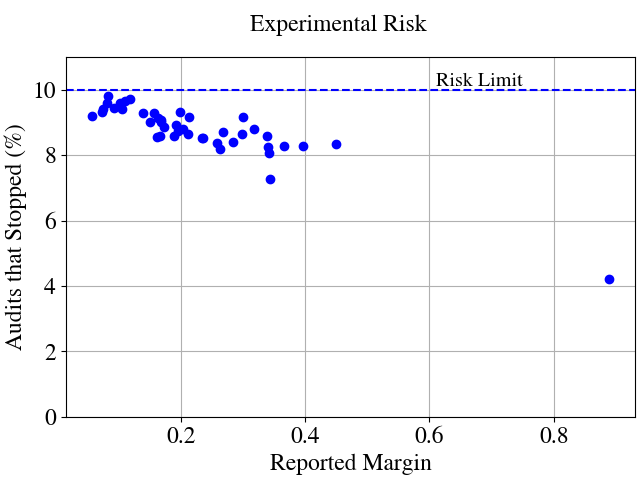
\includegraphics[width=.5\textwidth]{prov_risk.png}
\caption{The fraction of simulated \Providence audits on tied elections that stopped in any rounds (we performed five rounds at a $10\%$ risk limit). This value is an estimate of the maximum risk of the \Providence audit.}
\label{fig:prov-risk}
\end{figure}

In the simulations of \Providence audits of a tied election, the fraction of audits that stop, as shown in Figure~\ref{fig:prov-risk}, is an estimate of maximum risk. For all margins, this estimated maximum risk is less than the risk limit, supporting the claim that \Providence is risk-limiting.

\begin{figure}
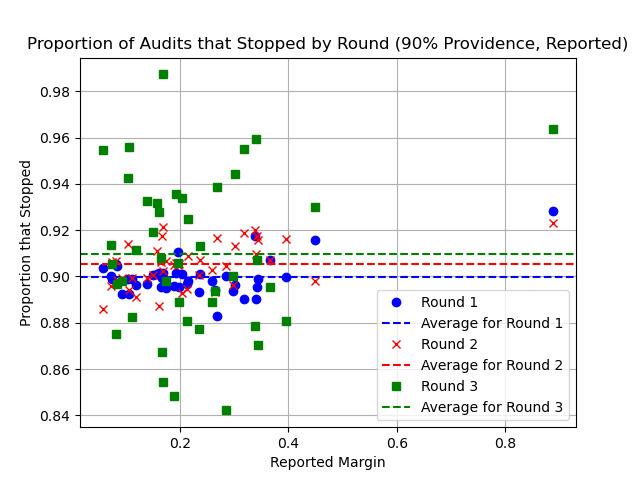
\includegraphics[width=.5\textwidth]{prov_sprob.png}
\caption{The fraction of simulated \Providence audits of the election as announced that stopped for each round. This value is an estimate of the stopping probability conditioned on the sample of the previous round. The average fraction for rounds 1, 2, and 3 is $89.96\%$, $90.52\%$, and $90.98\%$ respectively. We show only the first three rounds since so few audits make it to rounds 4 and 5.}
\label{fig:prov-sprob}
\end{figure}

Simulations of audits of the election as announced provide insight into stopping probability and number of ballots drawn when the election is as announced. We wish the stopping probability to be as predicted, and the number of ballots drawn to be small. Figure~\ref{fig:prov-sprob} shows that the stopping probabilities over the first rounds are near and slightly above $90\%$ as expected since our software chose round sizes to give at least a $90\%$ conditional stopping probability.

Figure~\ref{fig:prov-asn} plots the probability of stopping as a function of the number of ballots sampled. Points above (higher probability of stopping) and to the left (fewer ballots) represent more efficient audits. As shown, \Providence has comparable efficiency to \Minerva, while both are significantly more efficient than either implementation of \BRAVO. In a contest with a narrow margin (in the 2020 US Presidential election, eight states had margins less than $3\%$) the difference in number of ballots sampled could correspond to many days of work. 
% Section~\ref{sec:workload} discusses workload in more depth.

\begin{figure}
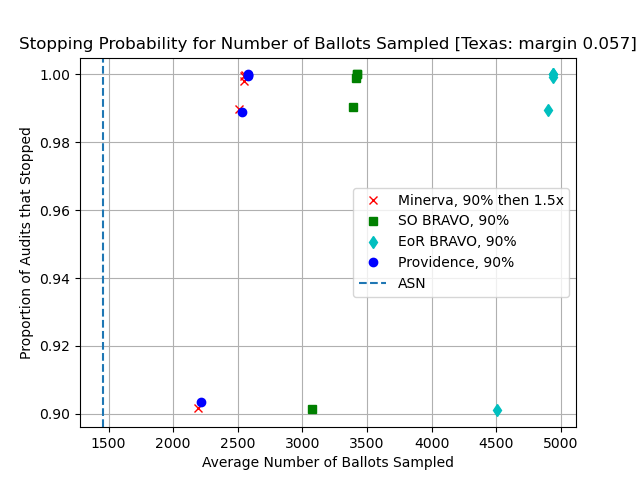
\includegraphics[width=.5\textwidth]{prov_asn.png}
\caption{For the entire audit, consisting of all five rounds, the estimated stopping probability for average number of ballots drawn for \Providence, \Minerva, EoR \BRAVO, and SO \BRAVO.}
\label{fig:prov-asn}
\end{figure}










\section{Pilot use}
\label{sec:pilot}
% pilot
A pilot audit was performed in Providence, Rhode Island in February 2022 of November 2021 special elections.
The audited contest was a yes-or-no question on School Construction and Renovation Projects and had an announced $25.67\%$ margin.
The risk-limit was $10\%$.
A first round size of $140$ ballots with large probability of stopping ($95\%$) was selected, and selection order was tracked, in order to give the potential for more interesting analysis afterwards. 
As expected, the audit concluded in the first round with a \Providence risk of $4.18\%$. Table~\ref{tab:pilot-risks} shows risk measures for the drawn sample using \Minerva and \BRAVO (both EoR and SO).

\begin{table}
\begin{center}
\begin{tabular}{ |c|c|c|c|c| } 
\hline
%\diagbox[dir=NW]{First \\Round \\Size}{RLA}
ballots& \rotatebox{45}{\Providence} & \rotatebox{45}{\Minerva} & \rotatebox{45}{EoR \BRAVO} & \rotatebox{45}{SO \BRAVO} \\
\hline
140 & \bf{4.18\%} & \bf{4.18\%} & \bf{5.41\%} & 36.6\% \\
\hline
\end{tabular}
\end{center}
\caption{Risk measures for the drawn first round of $140$ ballots in the Providence, RI pilot audit. Risks in bold meet the risk-limit ($10\%$) and thus correspond to audits that would stop.}
\label{tab:pilot-risks}
\end{table}

TODO: Add examples of how the audits perform for various hypothetical round schedules. I wait to do this until I'm done with the workload estimates since the examples here should be chosen to motivate that section.


\section{Audit workload}
\label{sec:workload}
Some election audits have benefited from a one-and-done approach: draw a large sample with high probability of stopping in the first round and usually avoid a second round altogether. This is appealing for two reasons. Firstly, rounds have some overhead in both time and effort. Thus the time and person-hours of an audit grows not just with the number of ballots sampled but also with the number of rounds. Secondly, smaller first round sizes are not large enough to accurately capture the distribution of votes. There is a higher probability that the true winner has fewer votes in the audit sample than some other candidate. On the other hand, a one-and-done audit may draw more ballots than are necessary; a more efficient round schedule could require less effort and time pre-certification. To evaluate the quality of various round schedules, we construct a simple workload model. Using this model we show how optimal round schedules can be chosen. We provide software that can be used by election officials to choose round schedules based on estimates of the model parameters like maximum allowed probability of a misleading audit sample.

As an example, we consider the US Presidential contest in the 2016 Virginia statewide general election. This contest had a margin of $0.053$ between the two candidates with the most votes.
Analytical approximation of the expected audit behavior (quantities like expected total number of ballots sampled or total number of rounds) is not straightforward. %challenging because the number of possible sequences of samples grows exponentially with the number of rounds. 
%A very rough approximation scheme is possible and may be useful when choosing round sizes in practice. We implement such a scheme, available at \cite{software}.
%We will use the more standard approach of simulations to give an example here.
Therefore we use the typical approach of simulations, again with risk limit $0.1$.

We simulate audits considering each candidate with a column in the results available at the Virginia Department of Elections website, including irrelevant ballots.
We consider a simple round schedule, in which each round is selected to give the same probability of stopping, $p$. That is, if the audit does not stop in the first round, we select a second round size which, given the sample drawn in the first round, will again have a probability of stopping $p$ in the second round. Note that since there are multiple candidates, we compute the minimum round size to achieve stopping probability $p$ for each pairwise contest between the winner and one of the losers, and we then select the largest such minimum round size and scale it up according to the proportion of the total ballots that are relevant to that pairwise contest. For this round schedule scheme, a one-and-done audit is achieved by choosing large $p$, say $p=.9$ or $p=.95$. We run $10^4$ trial audits for each value of $p$, assuming the reported results are correct\footnote{For this particular round schedule scheme, computing the expected number of rounds is straightforward analytically, but the expected number of ballots is still difficult, and so we use simulations.}. 

Note that simulations of audits of tied elections are not necessary, as all the audits we are considering are risk-limiting and hence we already know the performance to expect when auditing a tied election, even one not reported as such. 

Importantly, note that \Minerva does not appear in the analysis in this section. 
Questions about the efficiency of \Minerva for its necessarily fixed round schedules are addressed in section~\ref{sec:sims}, but in this section round sizes are chosen to have specified probabilities of stopping given previous samples. \Minerva is not known to be risk-limiting in this setting, and thus cannot be used for RLAs that proceed in this way.

\subsection{Person-hours}

\subsubsection{Average total ballots.} 
The simplest workload models are a function of just the total number of a ballots sampled\footnote{Sometimes total \emph{distinct} ballots sampled is used, but for the margins we use in our examples in this section, the difference between total distinct ballots and total ballots is very small\cite{arxiv_athena}. It is straightforward to modify the model we discuss here to account for total distinct ballots.}. Figure~\ref{fig:avg_bals} shows the average total number of ballots sampled as a function of $p$.
\begin{figure}[h!]
%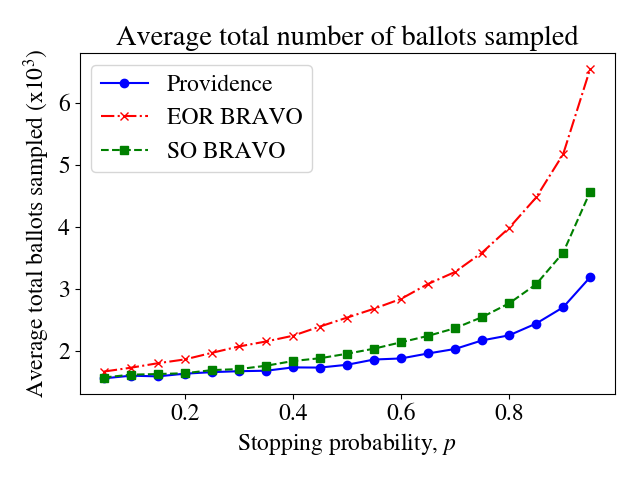
\includegraphics[width=.5\textwidth]{avg_bals.png}
%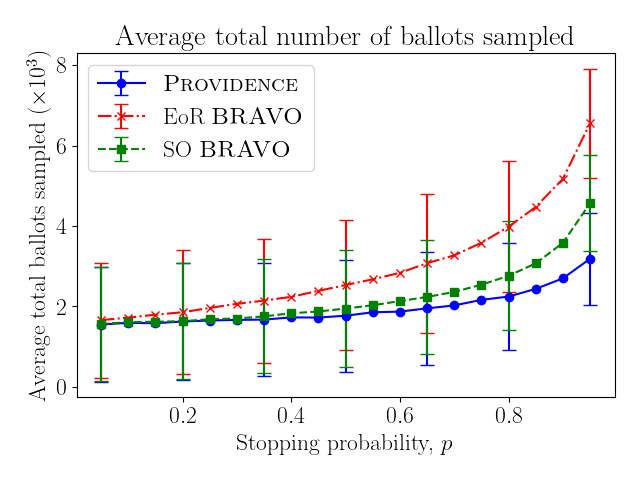
\includegraphics[width=.5\textwidth]{avg_bals_error_bars_every_three.png}
%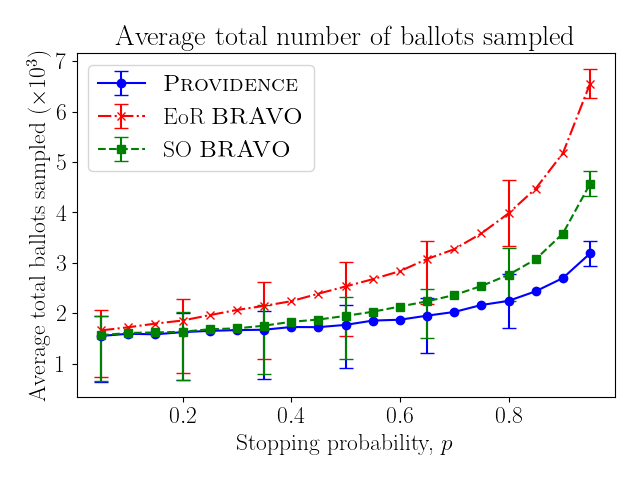
\includegraphics[width=.5\textwidth]{avg_bals_errorbars.png}
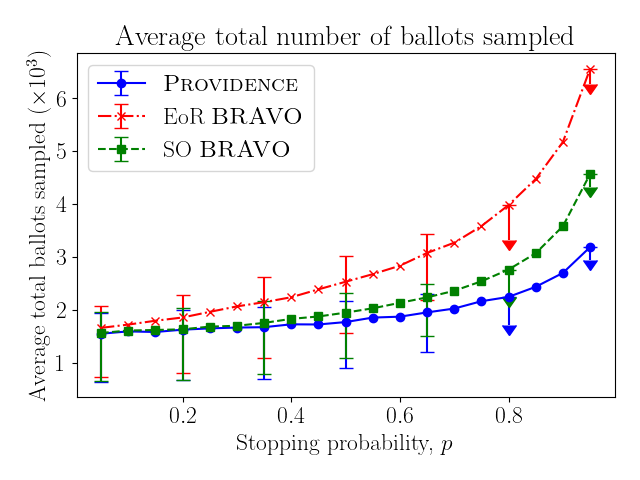
\includegraphics[width=.5\textwidth]{avg_bals_quantiles.png}
\caption{The average total number of ballots sampled, as a function of $p$, the conditional stopping probability used to select each round size, for ballot polling audits of the 2016 US Presidential election in the US State of Virginia. Error bars show the $0.25$ and $0.75$ quantiles. For sufficiently large $p$ ($p\ge 0.75$), the $0.25$ and $0.75$ quantiles are both equal to the first round size, and this is shown by the downward arrows.}
\label{fig:avg_bals}
\end{figure}

%Figure~\ref{fig:avg_bals_ratio} provides the same number as a fraction of the \Providence values.
It is straightforward to show that \Providence and both forms of \BRAVO collapse to the same test when each round corresponds to a single ballot. Figures~\ref{fig:avg_bals} 
%and \ref{fig:avg_bals_ratio} 
shows that for larger stopping probabilities $p$ (i.e. larger rounds), \Providence requires fewer ballots on average. In particular, the savings of \Providence become larger as $p$ increases; for $p=0.95$, EoR \BRAVO and SO \BRAVO require more than $2$ and $1.4$ times as many ballots as \Providence respectively. 

%\begin{figure}[h!]
%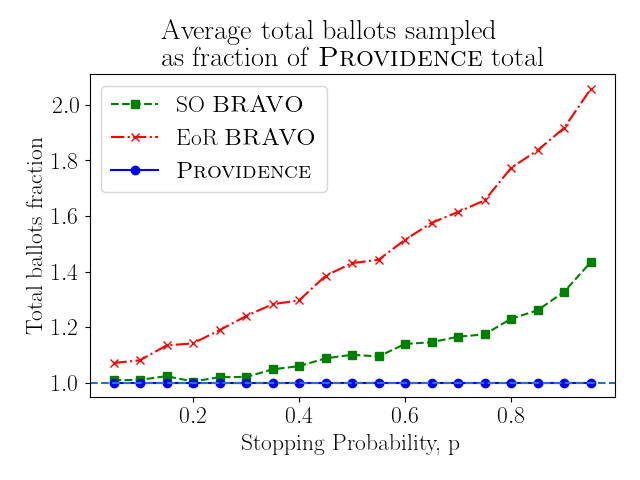
\includegraphics[width=.5\textwidth]{avg_bals_ratio.png}
%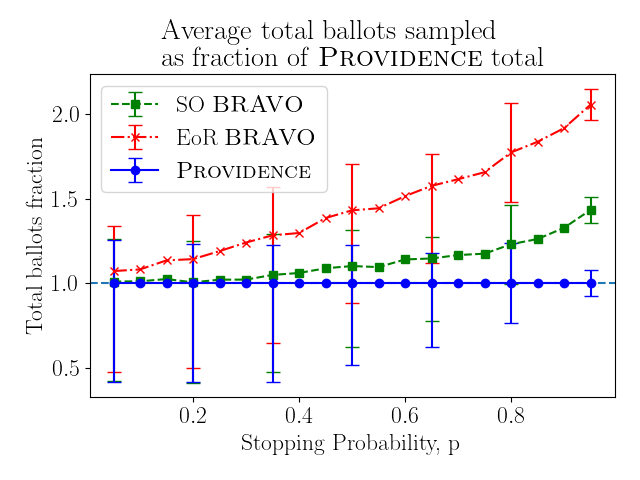
\includegraphics[width=.5\textwidth]{avg_bals_ratio_errorbars.png}
%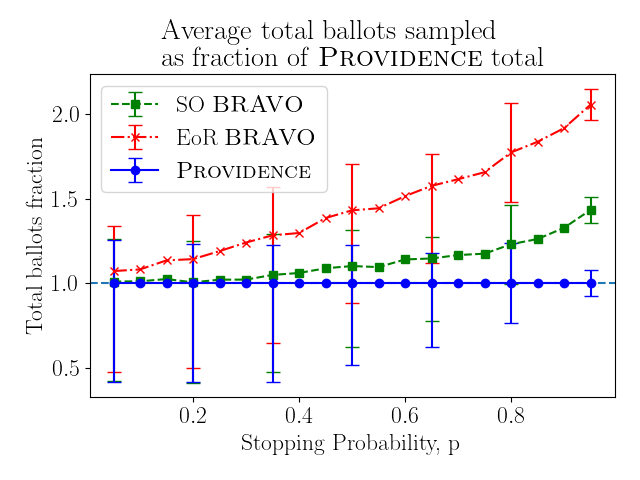
\includegraphics[width=.5\textwidth]{avg_bals_ratio_errorbars.png}
%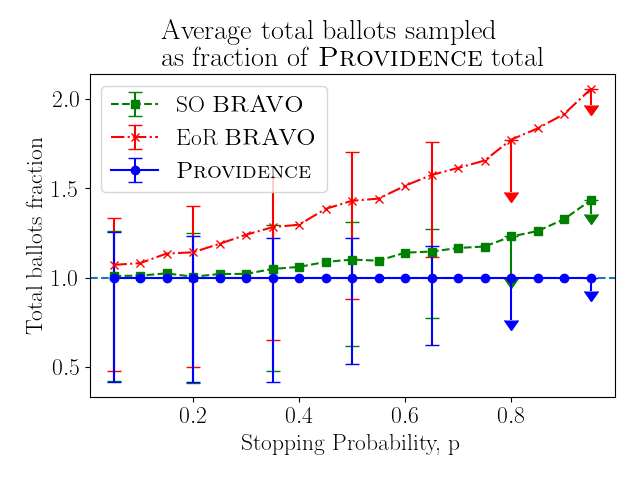
\includegraphics[width=.5\textwidth]{avg_bals_ratio_quantiles.png}
%\caption{The total number of ballots sampled on average, as a fraction of those sampled by \Providence, as a function of $p$, the conditional stopping probability used to select each round size, for ballot polling audits of the 2016 US Presidential election in the state of Virginia. The $0.25$ and $0.75$ quantiles are shown as in Figure~\ref{fig:avg_bals}.}
%\label{fig:avg_bals_ratio}
%\end{figure}


\subsubsection{Round overhead.} 
It is clear that average number of ballots alone is an inadequate workload measure. 
(Consider a state conducting its audit by selecting a single ballot at random, 
notifying just the county where the ballot is located, and then waiting to hear back for the manual interpretation of the ballot before moving on to the next one. 
This of course is inefficient and is why audits are actually performed in rounds.)

In a US state-wide RLA, the state organizes the audit by determining the random sample and communicating with the counties, but election officials at the county level physically sample and inspect the ballots after drawing them from secure storage boxes stored in county locations. 
Therefore each audit round requires some number of person-hours for set up and communication between state and county. This overhead for a round includes choosing the round size, generating the random sample, and communicating that random sample to the counties, as well as the communication of the results back to the state afterwards. 

Consequently, we now consider a model with a constant per-ballot workload $w_b$ and a constant per-round workload $w_r$.
So for an audit with expected number of ballots $E_{b}$ and expected number of rounds $E_{r}$, we estimate that the workload $W$ of the audit is
\begin{equation}
W(E_b,E_r) = E_b w_b + E_r w_r + C
\label{eq:round_workload}
\end{equation}

Note there is also some constant overhead of workload for the whole audit, namely $C$ in Equation~\ref{eq:round_workload}, which we take to be zero in our examples but could be used by election officials to represent, for example, the effort of constructing a ballot manifest.
For simplicity, (and without loss of generality), we measure in multiples of the per ballot workload; that is, we assume it is one unit, $w_b=1$. A per round workload of $w_r=x$ corresponds to a per round workload which is $x$ times the per ballot workload. We use $w_r=1000$ as a conservative example. 
That is, we set the overhead of a round equal to the workload of sampling $1000$ ballots. Based on available data\cite{RI-report}, the time retrieving and analyzing each individual ballot is on the order of $75$ seconds which means that $w_r=1000$ is equivalent to roughly $20$ person-hours of workload. This corresponds to about $15$ minutes being spent, on average, per round in each of the $133$ counties of Virginia, a clearly conservative workload estimate. We do not consider $w_r < 1$ because it is not possible for the round overhead to be smaller than the workload corresponding to a single ballot. 

As shown in Figure~\ref{fig:with_round_workload}, average workloads first reduce as stopping probability increases; this is likely due to a decrease in the number of rounds. After hitting a sweet spot, average workloads again increase with stopping probability; this time, likely because the average number of rounds does not decrease much and the cost changes because of number of ballots drawn, which increases with round size. \Providence achieves the lowest minimum average workload at roughly $p=0.7$ for our example choice of $w_r=1000$.

\begin{figure}[h!]
%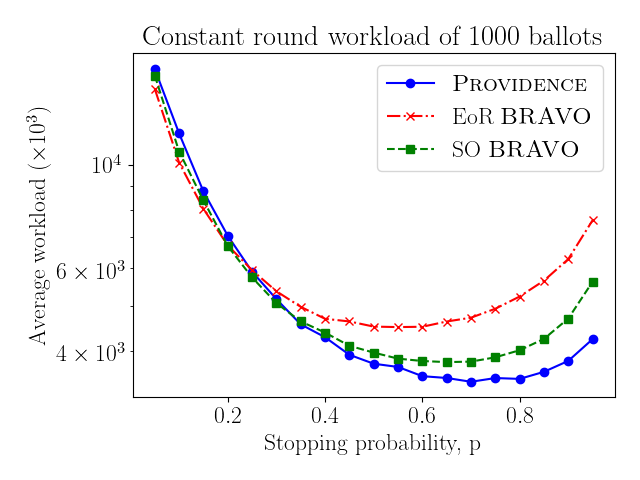
\includegraphics[width=.5\textwidth]{with_round_workload.png}
%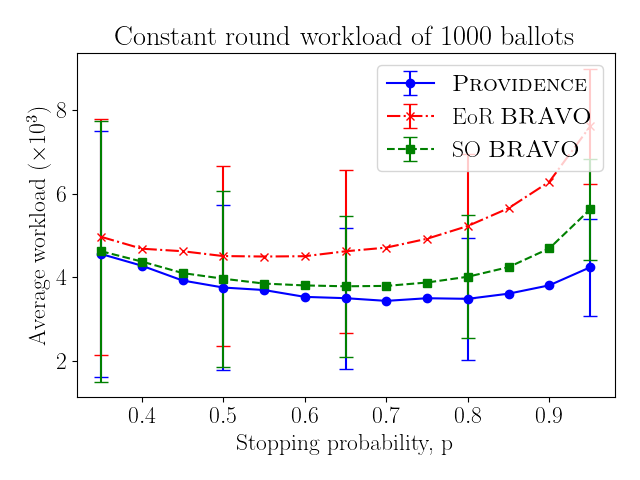
\includegraphics[width=.5\textwidth]{with_round_workload_errorbars.png}
%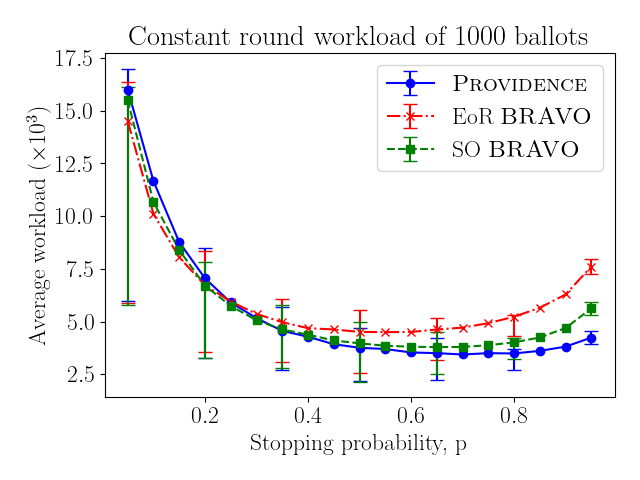
\includegraphics[width=.5\textwidth]{round_workload_errorbars.png}
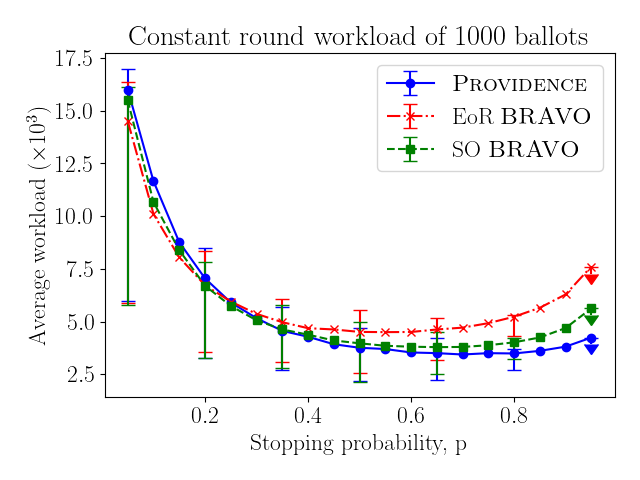
\includegraphics[width=.5\textwidth]{round_workload_quantiles.png}
\caption{For workload parameters $w_b=1$ and $w_r=1000$, this plot shows the expected workload for various values of $p$. Expected workload is found using Equation~\ref{eq:round_workload} and the average number of ballots and rounds in our simulations as the expected number of ballots and rounds. The $0.25$ and $0.75$ quantiles are shown as in Figure~\ref{fig:avg_bals}.}
\label{fig:with_round_workload}
\end{figure}

Importantly, this gives us a way to estimate the minimum expected workload, as well as which round schedule value $p$ achieves it, for arbitrary round workload. For each round workload $w_r$, we produce a dataset analagous to that of Figure~\ref{fig:with_round_workload} and then find the minimum average workload achieved for each of the audits and its corresponding stopping probability $p$. 

Figure~\ref{fig:optimal_workloads} shows the optimal achievable workload for a wide range of per round workloads. For very low round workloads, the workload function approaches just the total number of ballots, and so workload is minimized by minimizing the number of ballots drawn, which corresponds to small round sizes, and we would expect all three audits to behave similarly, as ballot-by-ballot audits, with the smallest workload. On the other hand, for extremely large values of round workload, the average number of ballots has little impact on the workload function, and so the three audits again have similar values, all corresponding to large round sizes in order to minimize the number of rounds.  We know that there is variation in the number of ballots used by each type of audit for large round sizes (a factor of two for $p=0.9$), but these values would be small in comparison to $w_r$. We observe this behaviour in Figure~\ref{fig:optimal_workloads} for extremely small and large workload values. For more reasonable values of the round workload $w_r$, SO \BRAVO and EoR \BRAVO achieve minimum workload roughly $1.1$ and $1.3$ times greater than that of \Providence.
\begin{figure}[h!]
%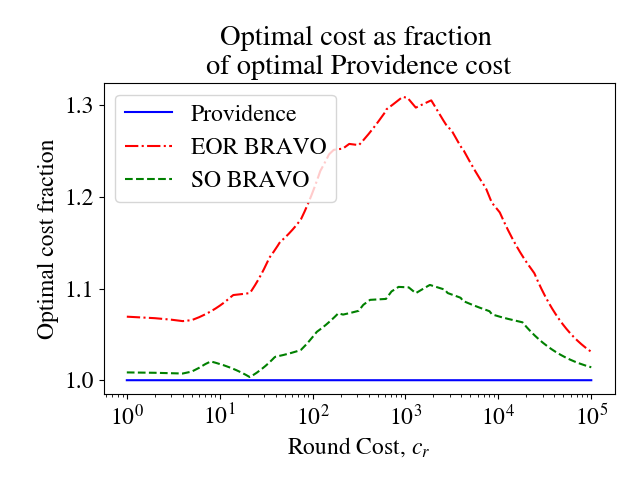
\includegraphics[width=.5\textwidth]{optimal_workloads.png}
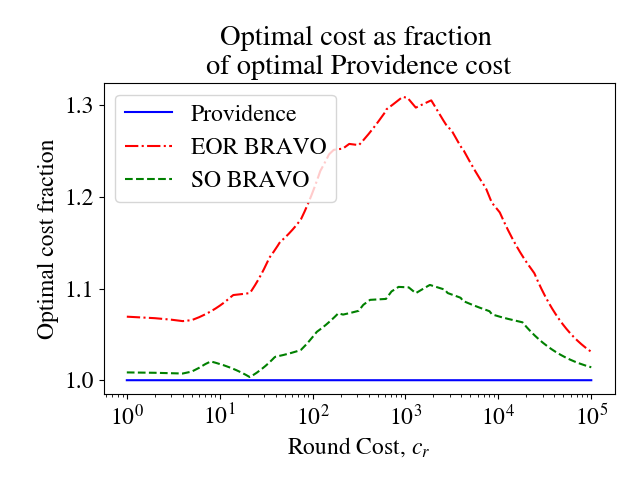
\includegraphics[width=.5\textwidth]{optimal_workloads.png}
\caption{For varying round workload $w_r$, the optimal average workload achievable by each audit, as a fraction of the \Providence values.}
\label{fig:optimal_workloads}
\end{figure}

Figure~\ref{fig:optimal_ps} shows the corresponding round schedule parameters $p$ that achieve these minimal workloads. As expected, an overhead for each round means that larger round sizes are needed to achieve an optimal audit, and so for all three audits $p$ increases as a function of $w_r$. Notice that \Providence is generally above and to the left of SO \BRAVO, and SO \BRAVO is generally above and to the left of EoR \BRAVO. This relationship reflects the fact that for the same round workload, \Providence can get away with a larger stopping probability because it requires fewer ballots.
\begin{figure}[h!]
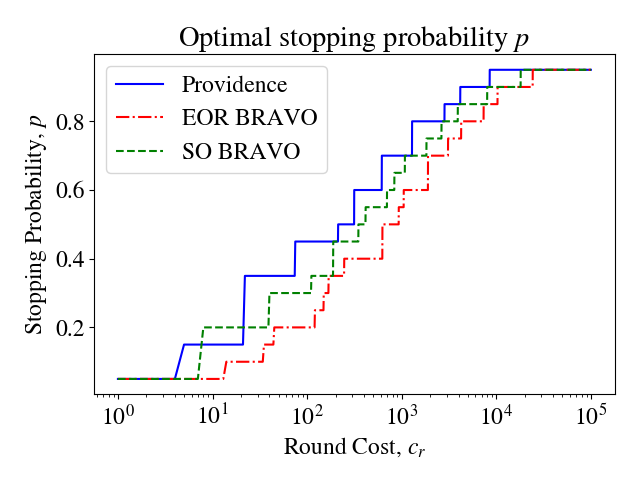
\includegraphics[width=.5\textwidth]{optimal_ps.png}
\caption{The optimal (workload-minimizing) stopping probability $p$ for varying workload model parameters $w_r$. (Note that the steps in this function are a consequence of our subsampling the workload function. That is, the workload-minimizing value of $p$ for each $w_r$ is only allowed to take on values at increments of $0.05$.)}
\label{fig:optimal_ps}
\end{figure}

\subsubsection{Precinct overhead.} For a more complete model, we can also introduce container-level workload. If a round requires multiple ballots from a single container, the container need only be unsealed once. Based on a Rhode Island pilot RLA report\cite{RI-report}, this may mean that a ballot from a new container requires roughly twice the time as a ballot from an already-opened container. Typically available election results give per-precinct granularity of vote tallies, rather than individual container information. In Virginia, however, most precincts have a single ballot scanner whose one box has sufficient capacity for all the ballots cast in that precinct anyways, and so we model the per-container workload as a per-precinct workload, $w_p$. In this model, the workload estimate incurs an additional workload of $w_p$ every time a precinct is sampled from for the first time in a round. That is, let $E_{pi}$ be the expected number of distinct precincts sampled from in round $i$, and let $E_p=\sum_i E_{pi}$. Then the new model is
\begin{equation}
W(E_b, E_r, E_p) = E_b w_b + E_r w_r + E_p w_p + C
\label{eq:round_and_precinct_workload}
\end{equation}

We can again explore the minimum achievable workloads under this model, as shown in Figure~\ref{fig:optimal_workload_precinct_workload_ratio}.

\begin{figure}
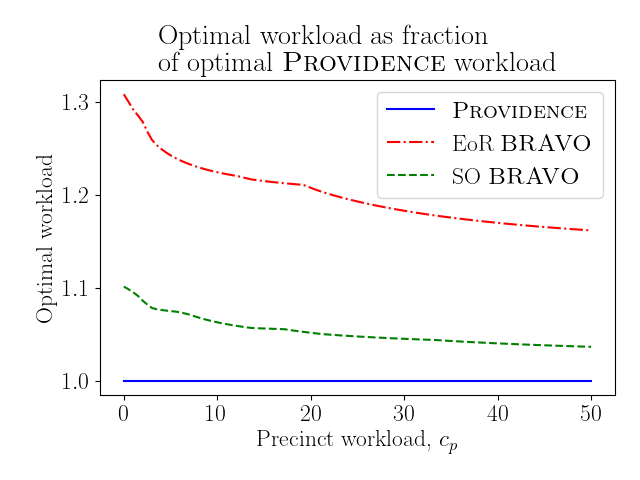
\includegraphics[width=.5\textwidth]{optimal_workload_precinct_workload_ratio.png}
\caption{Optimal average workload using the workload Equation~\ref{eq:round_and_precinct_workload} for varying $w_p$, given as a fraction of the value for \Providence. Similar to Figure~\ref{fig:optimal_workloads}, we show a generous range of values for the workload variable, $c_p$ in this case. If the time for a single ballot is $75$ seconds, then $c_p=50$ corresponds to over an hour of extra time to sample a ballot from a new container.}
\label{fig:optimal_workload_precinct_workload_ratio}
\end{figure}


\subsection{Real time}
Given tight certification deadlines,
%\footnote{Virginia recently passed legislation requiring pre-certification RLAs.}, 
the total real time to conduct the RLA is also an important factor to consider when planning audits.
Because each county can sample ballots for the same round concurrently, the total real time for a round depends only on the slowest county. 
In Virginia, Fairfax County typically has the most votes cast by a significant difference; in the contest we consider, Fairfax County had ~551 thousand votes cast, more than double the ~203 thousand of second-highest Virginia Beach City.
Consequently, we model the expected total real time $T$ of an audit using just the largest county, and we define analagous variables for the expected values in just the largest county.
Note that some other county may be slower, having fewer votes but also less auditing resources; but still, a slowest county exists. In this example, we take it to be Fairfax, the largest.
For the slowest county, let the expected total ballots sampled be $\bar E_b$, the expected number of rounds $\bar E_r$, and the expected number of distinct precinct samples summed over all rounds be $\bar E_p$.
Similarly, we use real time per-ballot, per-round, and per-precinct workload variables, $t_b$, $t_r$, and $t_p$. So the real time of the audit is estimated by
\begin{equation}
T(\bar E_b, \bar E_r, \bar E_p ) = \bar E_b t_b + \bar E_r t_r + \bar E_p t_p + C
\label{eq:real_time}
\end{equation}

As before, we can use our simulations to estimate $\bar E_b$, $\bar E_r$, and $\bar E_p$ using the corresponding averages over the trials. 
Available data to estimate values for $t_b$, $t_r$, and $t_p$ is limited, and so we take as an example the values $t_b=75$ seconds, $t_r=3$ hours, and $t_p=75$ seconds\footnote{The value $t_b=75$ seconds corresponds to a serial retrieval and interpretation of the ballots based on the \cite{RI-report} timing, $t_p=75$ seconds corresponds to the approximate doubling in time for new-box ballots as reported in \cite{RI-report} in the ballot-level comparison timing data, and $t_r=3$ hours is just a guess at an approximate order of magnitude for this variable.}. In practice, election officials could use our software and their own estimates of these values to explore choices for round schedules. Figure~\ref{fig:real_time} shows how the estimated real time for these values differs as a function of $p$. It should be noted that real values of $t_b$, $t_r$, and $t_p$ will vary greatly based on the number of parallel teams retrieving and checking ballots, the distribution of ballots and containers both in number and physical space, and other factors. We provide Figure~\ref{fig:real_time} only as an example of the general shape and behavior of this function. Use of this optimal scheduling tool would depend on parameter estimates tailored to each case.

\begin{figure}
%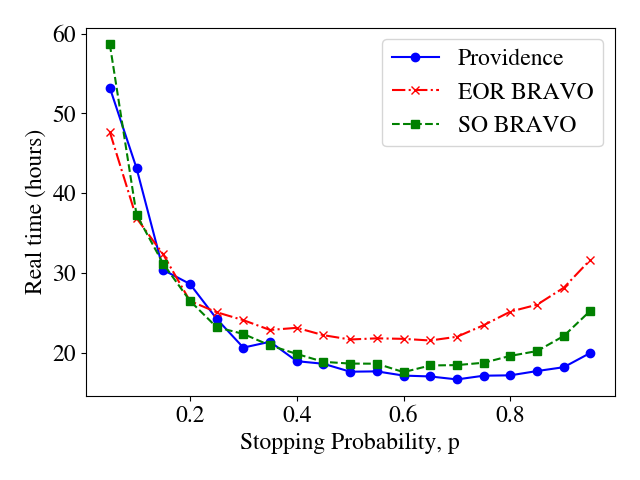
\includegraphics[width=.5\textwidth]{real_time.png}
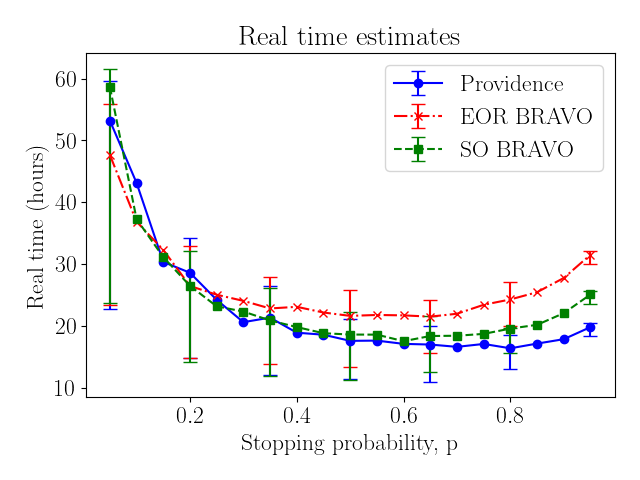
\includegraphics[width=.5\textwidth]{real_time_errorbars.png}
\caption{The real time as estimated by Equation~\ref{eq:real_time} for varying $p$ with expected values as estimated by our simulations. Error bars show the $0.25$ and $0.75$ quantiles. Unlike Figures \ref{fig:avg_bals}, \ref{fig:avg_bals_ratio}, and \ref{fig:with_round_workload}, the quantiles still differ for large $p$ because the first round size is no longer a constant; the number of ballots drawn in the first round in Fairfax County is variable.}
\label{fig:real_time}
\end{figure}


\section{Misleading samples}
\label{sec:misleading}

Unfortunately, efficiency alone is not sufficient for planning audits. In the US today, election officials have a legitimate need to include personal safety as a consideration.
In a random sample, a true loser may receive more votes than the true winner. This happens more often when the sample sizes are small, like for a hypothetical first round size of $11$ in the pilot audit, as seen in Figure~\ref{fig:pilot_sequence}.
In the abstract, a misleading sample in an early round is dealt with by drawing more ballots (moving on to another round), but in practice it serves to create expectations or suspicions that then need to be managed by election officials. Hence there is reason to structure round sizes so that they are unlikely to misrepresent the true outcome.

%, angry supporters of the losing candidate may be suspicious of election officials moving onto a next round, or, if the audit is declared correct after the second round, feel sufficiently disappointed to pose a threat. 
%but in practice the implications of this approach may be dangerous.

%Imagine that Alice beats Bob in an election contest both truly and in the reported results, but Bob's supporters are insistent he really won. When election officials carry out the RLA, they choose a small first round size in the hopes of achieving an efficient audit by getting to stop sooner (and drawing fewer ballots on average). 
% After the first round, by chance, there are more votes for Bob than for Alice in the sample. Bob's supporters celebrate their victory that the audit has in fact revealed that Bob really won, but the election officials have to explain that they are moving on to a second round. 

%After the second round, there are more votes in the sample for Alice and sufficiently many that the risk limit is met and the audit now ends confirming the announced result that Alice won. This is an undesirable situation, as it can appear to Bob's supporters that election officials are simply drawing ballots till a chosen outcome is obtained. 

We introduce the notion of a \emph{misleading sample}, any cumulative sample which, assuming the announced outcome is correct, contains more ballots for a loser than for the winner.
We can again use our simulations to gain insight into the frequency of \emph{misleading samples}.
For each stopping probability $p$, Figure~\ref{fig:misleading} gives the proportion of simulated audits that had a \emph{misleading sample} at any point. 
Notably, this proportion is as high as 1 in 5 for the smaller stopping probability round schedules.
Accordingly, we introduce a new parameter to our audit-planning tool, the maximum acceptable probability that the audit is misleading, the \emph{misleading limit}.

In Figure~\ref{fig:misleading}, horizontal lines are included to show \emph{misleading limits} of $0.1$, $0.01$, and $0.001$.
To achieve a probability of a misleading sample of at most $0.1$, a round schedule with at least roughly $p=.3$ is needed.
To achieve a probability of misleading of roughly $0.01$, a round schedule with $p=0.8$ is needed, and to achieve a probability of misleading of roughly $0.001$, a round schedule with $p=0.95$ is needed.
It is not unreasonable to think that election officials might choose a \emph{misleading limit} of $0.01$, or smaller, given the state of public perception of election security in the US and the associated threats of violence.
Consequently, the desired \emph{misleading limit} may be a deciding constraint in the choice of round schedule. 

\begin{figure}
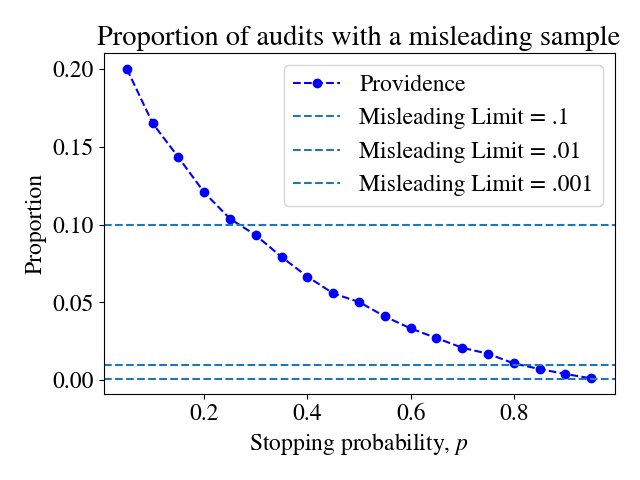
\includegraphics[width=.5\textwidth]{misleading_limits.png}
%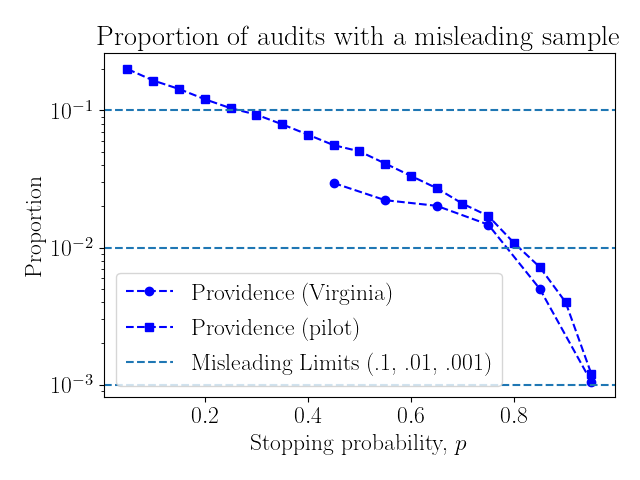
\includegraphics[width=.5\textwidth]{combined_misleading.png}
\caption{The proportion of simulated \Providence audits for the Virginia and pilot contest parameters that had a \emph{misleading sample} in any round.}
\label{fig:misleading}
\end{figure}

%We observe a similar behavior in our simulations of audits on the contest from the pilot audit. Figure~\ref{fig:misleading} also shows the proportion of the pilot simulations which contained a \emph{misleading sample} in any round. Despite the large difference in margin ($\sim 0.05$ in Virginia and $\sim 0.25$ in the pilot) we still observe that a \emph{misleading limit} of $0.01$ is first achieved at roughly $p=0.8$ and $0.001$ at $p=0.95$.

%\begin{figure}
%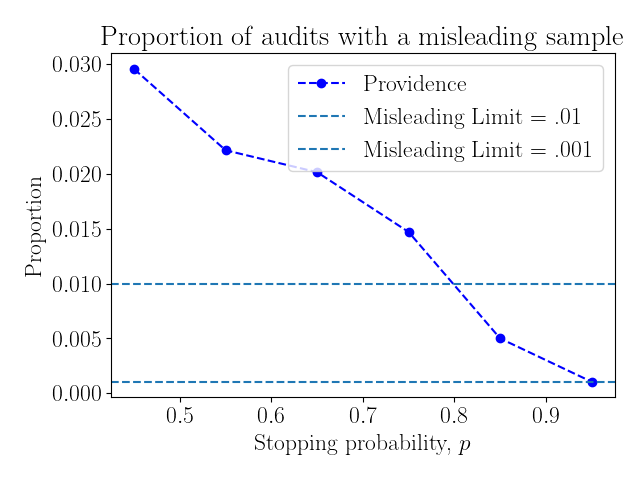
\includegraphics[width=.5\textwidth]{pilot_misleading_prop.png}
%\caption{The proportion of simulated \Providence audits for the pilot audit parameters that had a \emph{misleading sample} in any round.}
%\label{fig:pilot_misleading}
%\end{figure}

If election officials wish to enforce a \emph{misleading limit} for all the rounds, our simulation analysis could help. On the other hand, for a given round, it is straightforward to compute analytically the probability that a loser has more votes than the winner in the sample. Table~\ref{tab:misleading} shows for various margins the minimum first round size $n$ that guarantees a probability of a \emph{misleading sample} at most $M\in\{0.1,0.01,0.001\}$. For all values of $M$ and all margins, \Providence achieves a higher probability of stopping than either EoR \BRAVO or SO \BRAVO. 
    As seen in the Table~\ref{tab:misleading}, to enforce $M=0.01$ requires minimum round sizes with at least roughly a $0.8$ probability of stopping in the first round. Even if the most efficient audit schedule (by either workload or real time measures) would use a lower stopping probability $p$ to choose the first round size, the election officials may opt to use this constraint on the probability of a \emph{misleading sample} as the deciding factor in planning their audits.

\section{Conclusion}
\label{sec:conc}
%Conclusions
A rigorous tabulation audit is an important part of a secure election. Ballot polling RLAs are commonly used and simple, not relying on special election equipment like comparison RLAs. We present \Providence which is the most efficient and secure ballot polling RLA, as efficient as \Minerva  and flexible as \BRAVO. We present proofs and simulation results to verify the claimed properties of \Providence, and we provide an open source implementation of the stopping condition and useful related functionality.


\section{Availability}
\label{sec:avail}
\Providence is implemented in the open source R2B2 software library for \R and \B audits.\cite{r2b2}

\section{Acknowledgements}
\label{sec:ack}
The authors are grateful to the Rhode Island Board of Elections for conducting a pilot \Providence RLA. 
% The authors thank Georgina Cannan for insightful comments.

%-------------------------------------------------------------------------------
%\section{Introduction}
%%-------------------------------------------------------------------------------
%
%A paragraph of text goes here. Lots of text. Plenty of interesting
%text. Text text text text text text text text text text text text text
%text text text text text text text text text text text text text text
%text text text text text text text text text text text text text text
%text text text text text text text.
%More fascinating text. Features galore, plethora of promises.
%
%%-------------------------------------------------------------------------------
%\section{Footnotes, Verbatim, and Citations}
%%-------------------------------------------------------------------------------
%
%Footnotes should be places after punctuation characters, without any
%spaces between said characters and footnotes, like so.%
%\footnote{Remember that USENIX format stopped using endnotes and is
%  now using regular footnotes.} And some embedded literal code may
%look as follows.
%
%\begin{verbatim}
%int main(int argc, char *argv[]) 
%{
%    return 0;
%}
%\end{verbatim}
%
%Now we're going to cite somebody. Watch for the cite tag. Here it
%comes. Arpachi-Dusseau and Arpachi-Dusseau co-authored an excellent OS
%book, which is also really funny~\cite{arpachiDusseau18:osbook}, and
%Waldspurger got into the SIGOPS hall-of-fame due to his seminal paper
%about resource management in the ESX hypervisor~\cite{waldspurger02}.
%
%The tilde character (\~{}) in the tex source means a non-breaking
%space. This way, your reference will always be attached to the word
%that preceded it, instead of going to the next line.
%
%And the 'cite' package sorts your citations by their numerical order
%of the corresponding references at the end of the paper, ridding you
%from the need to notice that, e.g, ``Waldspurger'' appears after
%``Arpachi-Dusseau'' when sorting references
%alphabetically~\cite{waldspurger02,arpachiDusseau18:osbook}. 
%%
%It'd be nice and thoughtful of you to include a suitable link in each
%and every bibtex entry that you use in your submission, to allow
%reviewers (and other readers) to easily get to the cited work, as is
%done in all entries found in the References section of this document.
%
%Now we're going take a look at Section~\ref{sec:figs}, but not before
%observing that refs to sections and citations and such are colored and
%clickable in the PDF because of the packages we've included.
%
%%-------------------------------------------------------------------------------
%\section{Floating Figures and Lists}
%\label{sec:figs}
%%-------------------------------------------------------------------------------
%
%
%%---------------------------
%\begin{figure}
%\begin{center}
%\begin{tikzpicture}
%  \draw[thin,gray!40] (-2,-2) grid (2,2);
%  \draw[<->] (-2,0)--(2,0) node[right]{$x$};
%  \draw[<->] (0,-2)--(0,2) node[above]{$y$};
%  \draw[line width=2pt,blue,-stealth](0,0)--(1,1)
%        node[anchor=south west]{$\boldsymbol{u}$};
%  \draw[line width=2pt,red,-stealth](0,0)--(-1,-1)
%        node[anchor=north east]{$\boldsymbol{-u}$};
%\end{tikzpicture}
%\end{center}
%\caption{\label{fig:vectors} Text size inside figure should be as big as
%  caption's text. Text size inside figure should be as big as
%  caption's text. Text size inside figure should be as big as
%  caption's text. Text size inside figure should be as big as
%  caption's text. Text size inside figure should be as big as
%  caption's text. }
%\end{figure}
%%% %---------------------------
%
%
%Here's a typical reference to a floating figure:
%Figure~\ref{fig:vectors}. Floats should usually be placed where latex
%wants then. Figure\ref{fig:vectors} is centered, and has a caption
%that instructs you to make sure that the size of the text within the
%figures that you use is as big as (or bigger than) the size of the
%text in the caption of the figures. Please do. Really.
%
%In our case, we've explicitly drawn the figure inlined in latex, to
%allow this tex file to cleanly compile. But usually, your figures will
%reside in some file.pdf, and you'd include them in your document
%with, say, \textbackslash{}includegraphics.
%
%Lists are sometimes quite handy. If you want to itemize things, feel
%free:
%
%\begin{description}
%  
%\item[fread] a function that reads from a \texttt{stream} into the
%  array \texttt{ptr} at most \texttt{nobj} objects of size
%  \texttt{size}, returning returns the number of objects read.
%
%\item[Fred] a person's name, e.g., there once was a dude named Fred
%%%  who separated usenix.sty from this file to allow for easy
%%  inclusion.
%%\end{description}
%%
%%\noindent
%%The noindent at the start of this paragraph in its tex version makes
%it clear that it's a continuation of the preceding paragraph, as
%opposed to a new paragraph in its own right.
%
%
%\subsection{LaTeX-ing Your TeX File}
%%-----------------------------------
%
%People often use \texttt{pdflatex} these days for creating pdf-s from
%tex files via the shell. And \texttt{bibtex}, of course. Works for us.
%
%%-------------------------------------------------------------------------------
%\section*{Acknowledgments}
%%-------------------------------------------------------------------------------
%
%The USENIX latex style is old and very tired, which is why
%there's no \textbackslash{}acks command for you to use when
%acknowledging. Sorry.
%
%%-------------------------------------------------------------------------------


%%-------------------------------------------------------------------------------
%
%USENIX program committees give extra points to submissions that are
%backed by artifacts that are publicly available. If you made your code
%or data available, it's worth mentioning this fact in a dedicated
%section.
%
%-------------------------------------------------------------------------------
\bibliographystyle{plain}
\bibliography{audits.bib}




%appendix:

\appendix

\section{Proofs}
\label{sec:proofs}
\begin{lemma}
    \label{lemma:sigma_increasing}
For $0<p_0< p_a< 1$ and $n>0$, the ratio $\sigma(k,p_a,p_0,n)$ is strictly increasing as a function of $k$ for $0\le k\le n$.
\end{lemma}
\begin{proof}
See \cite[Lemma 4]{usenix_minerva}. 
\end{proof}

\begin{lemma}
    \label{lemma:frac_sums_increasing}
    Given a monotone increasing sequence: $\frac{a_1}{b_1}, \frac{a_2}{b_2}, \ldots, \frac{a_n}{b_n}$, for $a_i, b_i > 0$, the sequence:
    $$z_i = \frac{\sum_{j=i}^n a_j}{\sum_{j=i}^n b_j}$$
    is also monotone increasing.
\end{lemma}

\begin{proof}
See \cite[Lemma 2]{usenix_minerva}. 
\end{proof}

\begin{lemma}
    \label{lemma:tau1_increasing}
For $0<p_0< p_a< 1$ and $n>0$, the ratio $\tau_1(k,p_a,p_0,n)$ is strictly increasing as a function of $k$ for $0\le k\le n$.
\end{lemma}
\begin{proof}
    Apply Lemmas \ref{lemma:sigma_increasing}-\ref{lemma:frac_sums_increasing}.
\end{proof}
\begin{lemma}
    \label{lemma:imin-exists}
    Given a strictly monotone increasing sequence: $x_1, x_2, \ldots x_n $ and some constant $A$,
    %there exists an $i_{min}$ such that
    $$A \le x_i \Leftrightarrow \exists i_{min} \le i ~\text{s.t.}~   x_{i_{min} -1} < A \le x_{i_{min}} \le x_{i},$$
    unless $A\le x_1$, in which case $i_{min} =1 $.
\end{lemma}
\begin{proof}
    Evident.
\end{proof}

\begin{lemma}
    \label{lemma:minerva2_kmin_exists}
    For $\mathcal{A}=(\alpha,p_a, p_0,k_{j-1},n_{j-1},n_j)$-\Providence, there exists\\ a 
    $k^{p_a, p_0, \alpha, k_{j-1}}_{min, j, n_{j-1}, n_j}  = 
    k_{min,j}(\Providence, p_a, p_0, k_{j-1}, n_{j-1}, n_j)$ such that $$\mathcal{A}(X_j)=\text{Correct}\iff k_j\ge k_{min,j}(\Providence,  \bm{n_j}, p_a, p_0).$$
\end{lemma}
\begin{proof}
    From Definition~\ref{def:minervatwo}, $$\mathcal{A}(X_j)=\text{Correct}\iff \omega_j(k_{j}, k_{j-1}, p_a, p_0, n_j, n_{j-1}) \ge \frac{1}{\alpha}.$$
    Now to apply Lemma~\ref{lemma:imin-exists}, it suffices to show that
    $\omega_j$ is monotone increasing with respect to $k_j$.
    For $j=1$, we have $\omega_1=\tau_1$, so $\omega_1$ is strictly increasing by Lemma \ref{lemma:tau1_increasing}. For $j\ge 2$,
    $$\omega_j(k_j,k_{j-1},p_a,p_0,n_j,n_{j-1},\alpha)=$$$$\sigma(k_{j-1},p_a,p_0,n_{j-1})\cdot \tau_1(k_{j}-k_{j-1},p_a,p_0,n_j-n_{j-1}).$$
    As a function of $k_j$, $\sigma$ is constant, and thus $\omega$ is strictly increasing by Lemma \ref{lemma:tau1_increasing}. Therefore by Lemma \ref{lemma:imin-exists}, we have the desired property.
\end{proof}

\begin{lemma}
\label{lemma:any_ratio_is_sigma_simple}
For $j\ge 1$,
$$\frac{Pr[\bm{K_j}=\bm{k_j} \mid \bm{n_j}, H_a]}{Pr[\bm{K_j}=\bm{k_j} \mid \bm{n_j}, H_0]} = \sigma(k_j, p_a, p_0, n_j).$$
\end{lemma}
\begin{proof}
We induct on the number of rounds.
For $j=1$, we have
$$\frac{Pr[\bm{K_1}=\bm{k_1} \mid \bm{n_1},H_a]}{Pr[\bm{K_1}=\bm{k_1} \mid  \bm{n_1},H_0]} =\frac{Pr[K_1 = k_{1} \mid n_1,H_a]}{Pr[K_1 = k_1 \mid n_1,H_0]} $$$$= \frac{\text{Bin}(k_1,n_1,p_a)}{\text{Bin}(k_1,n_1,p_0)}=\sigma(k_1, p_a, p_0, n_1).$$
Suppose the lemma is true for round $j=m$ with history $\bm{k_m}$.
Observe that
 $$\frac{Pr[\bm{K_{m+1}}=\bm{k_{m+1}} \mid \bm{n_{m+1}},H_a]}{Pr[\bm{K_{m+1}}=\bm{k_{m+1}} \mid \bm{n_{m+1}}, H_0]} $$$$= \frac{ Pr[\bm{K_{m}}=\bm{k_{m}}\mid \bm{n_{m+1}},H_a] \cdot Pr[K_{m+1}'=k_{m+1}'|\bm{k_m},\bm{n_{m+1}},H_a]}{ Pr[\bm{K_{m}}= \bm{k_{m}} \mid  \bm{n_{m+1}},H_0]  \cdot  Pr[K_{m+1}'=k_{m+1}'|\bm{k_m},\bm{n_{m+1}},H_0]  }$$
 $$=\sigma(k_m, p_a, p_0, n_m) \cdot \frac{Pr[K_{m+1}'=k_{m+1}'|\bm{k_m}, \bm{n_{m+1}}, H_a]}{Pr[K_{m+1}'=k_{m+1}'|\bm{k_m},\bm{n_{m+1}},H_0]}$$
 by the induction hypothesis.
Then this is simply equal to
 $$\sigma(k_m, p_a, p_0, n_m)\cdot\frac{\text{Bin}(k_{m+1}',n_{m+1}',p_a)}{\text{Bin}(k_{m+1}',n_{m+1}',p_0)}
 $$$$
 =\frac{p_a^{k_m} (1-p_a)^{n_m-k_m}}{p_0^{k_m} (1-p_0)^{n_m-k_m}} \cdot
 \frac{p_a^{k_{m+1}'} (1-p_a)^{n_{m+1}'-k_{m+1}'}}{p_0^{k_{m+1}'} (1-p_0)^{n_{m+1}'-k_{m+1}'}}
 $$
 $$
 =\sigma(k_{m+1}, p_a, p_0, n_{m+1})
 $$
\end{proof}


\begin{definition} 
\label{def:kmin}
Let $[n_1, \ldots, n_j]$ be the round schedule of an audit that has not stopped by the round $j-1$. Let us define 
\begin{small}
\begin{equation}\label{eq:kMin}
k^{p_a, p_0, \alpha, k_{j-1}}_{min, j, n_{j-1}, n_j}  =
  \min\left\{k : \omega_j(k, k_{j-1},p_a,p_0,n_j, n_{j-1}) \geq \frac{1}{\alpha}  \right\}.
%  \min\left\{k : \sigma(k_{r-1},p_a,p_0,n_{r-1})\cdot \tau_1(k-k_{r-1},p_a,p_0,n_r-n_{r-1}) \geq \frac{1}{\alpha}  \right\}$
\end{equation}
\end{small}
\end{definition}
As we have seen in Lemma \label{lemma:minerva2_kmin_exists}, such a value of $k^{p_a, p_0, \alpha, k_{j-1}}_{min, j, n_{j-1}, n_j}$ exists and $k_j \geq k^{p_a, p_0, \alpha, k_{j-1}}_{min, j, n_{j-1}, n_j} $ if and only if the result of the audit is Correct, (\textit{i.e.,} the stopping condition in Definition~\ref{def:minervatwo} holds).

The following lemma shows a Markov-like property of \Providence audit (\textit{i.e.,}
for an audit that has not stopped in the first $j-1$ rounds, only cumulative results of the round $j-1$ matter: cumulative sample size $n_{j-1}$ and the number of ballots for the winner $k_{j-1}$).

\begin{lemma}\label{lemma:markov}
Let $[n_1, \ldots, n_{j-1}, n_j]$ be a round schedule for an execution of  \Providence audit that has not stopped
in any of its first $j-1$ rounds (\textit{i.e.,} for every $i = 1, \ldots, j-1$:
$k_i < k^{p_a, p_0, \alpha, k_{j-1}}_{min, j, n_{j-1}, n_j} $), then: 

\[ 
k^{p_a, p_0, \alpha, k_{j-1}}_{min, j, n_{j-1}, n_j} = k^{p_a, p_0, \alpha, k_{j-1}}_{min, 2, n_{j-1}, n_j} .
\]
\end{lemma}
% \fpo{this can be used to prove that \Providence is more efficient than \Minerva and \BRAVO}
\begin{proof}
Let $k_{j-1}$ denote the number of ballots drawn for the declared winner up to the round $j-1$ (out of $n_{j-1}$ sampled ballots). The stopping decision for the round $j$ is made as follows:

\[
 k^{p_a, p_0, \alpha, k_{j-1}}_{min, j, n_{j-1}, n_j}  = \min\left\{k : \omega_{j}(k, k_{r-1}, p_a, p_0, n_r, n_{r-1}) \geq \frac{1}{\alpha}  \right\} = 
\]
\[
  =  k^{p_a, p_0, \alpha, k_{j-1}}_{min, 2, n_{j-1}, n_j}  
\]

\end{proof}

That is, the stopping condition is equivalent to that of a two round audit with the same cumulative votes for the winner and cumulative round sizes: the first round is of size $n_{j-1}$ and has $k_{j-1}$ votes for the winner, and the second (cumulative) round size is $n_j$ with $k_j$ (cumulative) votes for the winner. Compare this to the similar property for the $\Bravo$ stopping condition. 




%%%%%%%%%%%%%%%%%%%%%%%%%%%%%%%%%%%%%%%%%%%%%%%%%%%%%%%%%%%%%%%%%%%%%%%%%%%%%%%%
\end{document}
%%%%%%%%%%%%%%%%%%%%%%%%%%%%%%%%%%%%%%%%%%%%%%%%%%%%%%%%%%%%%%%%%%%%%%%%%%%%%%%%

%%  LocalWords:  endnotes includegraphics fread ptr nobj noindent
%%  LocalWords:  pdflatex acks
% Following each round, a decision is taken whether to end the audit, declaring it successful and the election correct, or to draw another round of ballots. The votes would be fully hand counted after multiple unsuccessful rounds. Real ballot polling RLAs draw ballots in rounds of multiple ballots each. 



% Template for USENIX papers.
%
% History:
%
% - TEMPLATE for Usenix papers, specifically to meet requirements of
%   USENIX '05. originally a template for producing IEEE-format
%   articles using LaTeX. written by Matthew Ward, CS Department,
%   Worcester Polytechnic Institute. adapted by David Beazley for his
%   excellent SWIG paper in Proceedings, Tcl 96. turned into a
%   smartass generic template by De Clarke, with thanks to both the
%   above pioneers. Use at your own risk. Complaints to /dev/null.
%   Make it two column with no page numbering, default is 10 point.
%
% - Munged by Fred Douglis <douglis@research.att.com> 10/97 to
%   separate the .sty file from the LaTeX source template, so that
%   people can more easily include the .sty file into an existing
%   document. Also changed to more closely follow the style guidelines
%   as represented by the Word sample file.
%
% - Note that since 2010, USENIX does not require endnotes. If you
%   want foot of page notes, don't include the endnotes package in the
%   usepackage command, below.
% - This version uses the latex2e styles, not the very ancient 2.09
%   stuff.
%
% - Updated July 2018: Text block size changed from 6.5" to 7"
%
% - Updated Dec 2018 for ATC'19:
%
%   * Revised text to pass HotCRP's auto-formatting check, with
%     hotcrp.settings.submission_form.body_font_size=10pt, and
%     hotcrp.settings.submission_form.line_height=12pt
%
%   * Switched from \endnote-s to \footnote-s to match Usenix's policy.
%
%   * \section* => \begin{abstract} ... \end{abstract}
%
%   * Make template self-contained in terms of bibtex entires, to allow
%     this file to be compiled. (And changing refs style to 'plain'.)
%
%   * Make template self-contained in terms of figures, to
%     allow this file to be compiled. 
%
%   * Added packages for hyperref, embedding fonts, and improving
%     appearance.
%   
%   * Removed outdated text.
%
%%%%%%%%%%%%%%%%%%%%%%%%%%%%%%%%%%%%%%%%%%%%%%%%%%%%%%%%%%%%%%%%%%%%%%%%%%%%%%%%


\documentclass[letterpaper,twocolumn,10pt]{article}
\usepackage{usenix-2020-09}

% to be able to draw some self-contained figs
\usepackage{tikz}
\usepackage{amsmath}
\usepackage{thmtools,thm-restate}

\usepackage{tabularx}

% inlined bib file
\usepackage{filecontents}

\usepackage{xspace}
\usepackage{diagbox}
\usepackage{comment}
\usepackage{authblk}
\usepackage{times}
\usepackage{amsmath,amsfonts,amssymb,amsthm}
\usepackage{graphicx}
\newtheorem{lemma}{Lemma}
\newtheorem{theorem}{Theorem}
\newtheorem{corollary}{Corollary}
\newtheorem{proposition}{Proposition}
\newtheorem{definition}{Definition}
\newtheorem{theoremA}{Theorem}
\usepackage[normalem]{ulem}
\usepackage{mathtools}
\usepackage{authblk}
\usepackage{times}
\usepackage{amsmath, amsthm, graphicx, comment, xspace, amssymb}
\usepackage{bm}

\graphicspath{{./imgs/}}

% \newtheorem{example}{Example}

\theoremstyle{definition}
\newtheorem{example}{Example}

% nice looking audit titles
\newcommand{\Minerva}{\textsc{Minerva}\xspace}
\newcommand{\Providence}{\textsc{Providence}\xspace}
\newcommand{\B}{{{B2}}\xspace}
\newcommand{\R}{{{R2}}\xspace}
\newcommand{\BRAVO}{\textsc{Bravo}\xspace}
\newcommand{\fpo}[1]{\marginpar{\scriptsize\textcolor{red}{fpo: #1}}}
\newcommand{\Bravo}{\textsc{Bravo}\xspace}

%-------------------------------------------------------------------------------
%\begin{filecontents}{\jobname.bib}
%%-------------------------------------------------------------------------------
%@Book{arpachiDusseau18:osbook,
%  author =       {Arpaci-Dusseau, Remzi H. and Arpaci-Dusseau Andrea C.},
%  title =        {Operating Systems: Three Easy Pieces},
%  publisher =    {Arpaci-Dusseau Books, LLC},
%  year =         2015,
%  edition =      {1.00},
%  note =         {\url{http://pages.cs.wisc.edu/~remzi/OSTEP/}}
%}
%@InProceedings{waldspurger02,
%%  author =       {Waldspurger, Carl A.},
%  title =        {Memory resource management in {VMware ESX} server},
%  booktitle =    {USENIX Symposium on Operating System Design and
%                  Implementation (OSDI)},
%%  year =         2002,
%  pages =        {181--194},
%  note =         {\url{https://www.usenix.org/legacy/event/osdi02/tech/waldspurger/waldspurger.pdf}}}
%\end{filecontents}
%
%%%-------------------------------------------------------------------------------
\begin{document}
%-------------------------------------------------------------------------------

%don't want date printed
\date{}

% make title bold and 14 pt font (Latex default is non-bold, 16 pt)
\title{\Large \bf \Providence: a Flexible Round-by-Round Risk-Limiting Audit}
%\author{
%{\rm Oliver Broadrick$^1$\thanks{odbroadrick@gmail.com}, Poorvi L. Vora$^1$, and Filip Zag{\'o}rski$^{23}$}\\
%$^1$Department of Computer Science, The George Washington University\thanks{Authors supported in part by NSF Award 2015253}\\
%$^2$University of Wroclaw\\
%$^3$Votifica
% copy the following lines to add more authors
% \and
% {\rm Name}\\
%Name Institution
%} % end author
\maketitle

%-------------------------------------------------------------------------------
%\begin{abstract}
%-------------------------------------------------------------------------------
%Your abstract text goes here. Just a few facts. Whet our appetites.
%Not more than 200 words, if possible, and preferably closer to 150.
%\end{abstract}
\begin{abstract}
A Risk-Limiting Audit (RLA) is a statistical election tabulation audit with a rigorous error guarantee. We present ballot polling RLA \Providence, an audit with the efficiency of \Minerva and flexibility of \BRAVO, and prove that it is risk-limiting in the presence of an adversary who can choose subsequent round sizes given knowledge of previous samples. We describe a measure of audit workload as a function of the number of rounds, precincts touched, and ballots drawn and quantify the problem of obtaining a misleading audit sample when rounds are too small, demonstrating the importance of the resulting constraint on audit planning. We describe an approach to planning audit round schedules using these measures and present simulation results demonstrating the superiority of \Providence. 

We describe the use of \Providence by the Rhode Island Board of Elections in a tabulation audit of the 2021 election. 
Our implementation of \Providence 
% and audit planning tools 
in the open source R2B2 library has been integrated as an option in Arlo, the most commonly used RLA software.

%should be useful to the states of Georgia and Pennsylvania, which are planning pre-certification ballot polling RLAs for the 2022 general election. 
% footnotes not common in abstracts. This footnote not sufficiently compelling: \footnote{https://www.brennancenter.org/our-work/analysis-opinion/poll-local-election-officials-finds-safety-fears-colleagues-and}.
% and integrated into Arlo, election audit software used across the US.
%\keywords{risk-limiting audit (RLA)  \and ballot polling audit \and evidence-based elections \and statistical election audit}
\end{abstract}
%
%

\section{Introduction}
\label{sec:intro}
%Intro
It is well-known that electronic voting systems are vulnerable to software errors and manipulation which may be undetected. Errors and/or manipulation may not always change an election outcome, but we would want to know when they do. {\em Software independent} voting systems \cite{SI-Wack,rivest2008notion} are ones where an undetected change in the software cannot lead to an undetectable change in the election outcome. {\em Evidence-based elections} \cite{evidence-based} use software independent systems to produce trustworthy evidence of outcome correctness; incorrect outcomes are detected with high probability when the evidence is examined. One approach to evidence-based elections is to use voter-verified paper ballots, store them securely, and perform public audits---a compliance audit to determine whether the ballots were stored securely; and a rigorous tabulation audit, known as a risk-limiting audit (RLA) \cite{RLA}, to determine whether the outcome is correctly computed from the stored ballots.  A {\em risk-limiting audit} guarantees a minimum probability of a full hand count if the election outcome is incorrect. Conversely, it guarantees a maximum probability of audit error, termed the {\em risk limit}, which is the maximum probability with which the audit would declare an incorrect election outcome as being correct. 

Many US states have had pilot RLA programs. Additionally, some states allow RLAs to be used towards audit requirements, and some states require RLAs before elections can be certified. 

%We propose the \Providence audit, a new approach to a particular type of RLA---the ballot polling RLA described below---and propose a new model for the work load of an election. We show that \Providence is superior to the popular ballot polling RLA \Bravo for real elections, and describe the use of our open source implementation by the Rhode Island Board of Elections for an audit of their 2021 elections. \Providence was recently integrated as an option in Arlo \cite{arlo}, the most popular election audit software. %Our open-source implementations of \Providence and our audit planning tools are likely to be useful later this year; ballot polling audits are expected to be used as pre-certification RLAs in at least one statewide contest in both Georgia and Pennsylvania for the 2022 general elections in the US.   

\subsection{Background on RLAs}
We provide here the background necessary to evaluate our contributions. 

All RLAs sample one or more ballots at random; we will refer to each such set of ballots as a {\em round}. The ballots are manually examined, and a stopping condition computed, which determines whether (a) the audit ends in success (the election outcome is declared correct) or (b) another round should be drawn (more information is needed before a determination). In principle, the stopping condition could indicate a third option too: (c) the audit proceeds to a full manual hand count. However, a manual hand count presents significant logistical challenges, and there is always a chance that it will have been unnecessary, hence (c) is generally not incorporated. Election officials would typically decide to perform a full manual hand count if the audit does not stop in spite of drawing a large number of ballots, typically over multiple rounds. They would be influenced by the certification deadline, the estimated number of human hours required for another round, the logistical costs of a full hand count, and the impact of any decision on citizen confidence. 

\subsubsection{Types of RLAs}
In a ballot comparison RLA \cite{RLA}, the manual interpretation of each sampled ballot is compared to the corresponding Cast Vote Record (CVR), which is the machine interpretation of the ballot. Ballot comparison RLAs require the fewest ballots of all known RLA approaches, but also require a means of identifying the CVR corresponding to a particular ballot. A typical approach is to use a ballot serial number on both paper ballot and CVR. When voters vote in precincts, however, serial numbers on ballots can enable the correlation of ballots with voters, and ballots are typically not numbered. Additionally, some voting systems do not record a CVR. One may perform a transitive audit by rescanning unnumbered voted ballots with special scanners which produce CVRs and also print numbers on the ballots as they are scanned. This requires an investment in a sufficiently large number of such printers and in the human effort of rescanning ballots, and is not always feasible. 

In a ballot polling RLA \cite{RLA}, the manual interpretations of the sampled ballots are simply tallied. Ballot polling RLAs require a much larger number of ballots than ballot comparison RLAs, but are more feasible because they do not require any additional functionality of the voting system, and, in particular, do not need CVRs. What is needed is a complete ballot manifest (a list of ballot storage containers and the number of ballots in each) which enables the creation of a well defined list of the ballots and their locations (the fifth ballot in box number 20, for example).  

A batch comparison RLA \cite{RI-report} samples batches of ballots (typically, a batch is a storage box of ballots) and compares the manual tally of each sampled batch with the announced tally of that batch. Thus, while this type of audit does not need CVRs, it does need both a ballot manifest and a public declaration of the tally of each batch. This approach typically requires the sampling of a very large number of ballots. However, the process is most similar to that which election officials already use when they perform fixed-percentage post-election audits, where, for example, 2\% of the batches are manually tallied. (Note that, for an RLA, the number of batches tallied is not fixed; the risk limit is. A smaller number of batches might be sufficient, or a larger number necessary, for an audit with the required risk limit.)

This paper focuses on ballot polling RLAs which have been used in a number of US state pilots (California, Georgia, Indiana, Michigan, Ohio, Pennsylvania, Virginia and elsewhere) and in real statewide audits (Georgia, Virgina) \cite{vv_audits} as well as in audits of smaller jurisdictions, such as Montgomery County, Ohio \cite{usenix_minerva}. 

\subsubsection{Ballot Polling Audits}
Ballot polling audits proceed as follows. 
\begin{enumerate}
\item A first round \cite{usenix_minerva} size---the number of ballots sampled before first checking the stopping condition---is chosen. 
\item Ballots on the ballot manifest are sampled uniformly at random using a pseudorandom number generator typically seeded by a natural source of randomness like rolling dice.
\item The physical ballots are found and manually interpreted, recording the manual interpretations. 
\item Based on the manual interpretations, the stopping condition is computed. 
\item If more ballots are to be drawn, the next round size is chosen. Round sizes, including the first one, may be computed based on a desired probability of audit completion at the end of the round, and may take into consideration loose estimates of the resources required. For RLAs required by statute or law, certification deadlines would play a large role, as the audit would need to be completed before the deadline. 
\end{enumerate} 

A {\em round-by-round (R2)} audit is the general audit, where the decision of whether to draw more ballots or not is taken after drawing a round of ballots; typically hundreds or thousands or tens of thousands of ballots in statewide elections. A {\em ballot-by-ballot (B2)} audit is the special case of round size one---when the decision is made after each ballot is drawn. The popular \BRAVO audit requires the smallest expected number of ballots when the announced tally of the election is correct, and stopping decisions are taken a ballot at a time (that is, when it is used as a B2 audit). 

Election officials typically draw ballots in large round sizes:  see for example \cite{va-2022,RI-report}, and note that, in addition to allowing users to directly enter a round size, Arlo provides choices of stopping probabilities of $0.9$, $0.8$ and $0.7$, and the expected number of ballots required by \BRAVO. Further, at both audits we attended, election officials chose stopping probabilities of $0.9$ and we are not aware of any ballot polling RLA performed on ballots cast in a governmental election that drew ballots one at a time (though the stopping condition can be computed one ballot at a time, the ballots are drawn in rounds). \BRAVO hence cannot be used as a B2 audit in these scenarios. 

For use as an R2 audit, the \BRAVO stopping condition can be applied once at the end of each round (End-of Round (EoR)), or retroactively after each ballot drawn if ballot order is retained (Selection-Ordered (SO)). SO \BRAVO is closer to the original B2 \BRAVO, and requires fewer ballots on average than EoR \BRAVO. But it requires the additional effort of tracking the order of ballots. 

\subsubsection{Adversarial Model for RLAs}
Detailed descriptions of best practices for post-election audits may be found in \cite{best-practices,why-and-how}. For our purposes, we will assume that the best practices are followed: the paper trail consists of hand-marked paper ballots and is secured; a public compliance audit is carried out before the RLA to ensure that the processes for securing the paper trail were followed; voter authentication and registration processes were verified, and only legitimate voters cast no more than a single vote each; the risk-limiting audit is public. We will further assume that all software used in the RLA is open source and well-defined, so its output may be reproduced and thus verified by an observer wishing to do so with their own software. 

Referring to the ballot polling audit steps described above, we further assume that a secure PRNG is used; the seed is generated uniformly at random in a public process; the process of locating ballots is publicly observable and the located ballots can be viewed by the public. Because the PRNG is well-defined, as is the stopping condition, we may assume that the stopping condition is correctly computed from knowledge of the seed and the drawn ballots. Thus the only variable is round size. We define a {\em weak adversary} as one who can choose the first round size and a {\em strong adversary} as one who can choose any round size. 

\subsection{The Literature and Open Questions}
Zag\'{o}rski {\em et al.} propose ballot polling RLA \Minerva \cite{usenix_minerva}, which does not need ballot order and relies only on sample and round tallies. They prove that it is risk-limiting when the number of relevant ballots drawn in each round is pre-determined before any ballots are examined; that is, for a weak adversary. They do not address the case of a strong adversary (such as an audit insider) who can determine the size of the next round after knowing what votes are on the ballots sampled thus far. In particular, an open question about \Minerva is whether the computation of a risk limit assuming a weak adversary applies to an attack by a strong adversary, or is the risk limit computation incorrect when the adversary is strong? Can the strong adversary increase the audit's error probability beyond its declared risk limit? Or is there no probabilistic adversarial advantage to being able to compute next round sizes after knowing the drawn sample? We do not answer this question, and to our knowledge, it remains open. 

Until \Minerva is proven to be risk-limiting to a given risk limit for the strong adversary, it may not be used in audits whose round sizes are not pre-determined. This presents a major limitation, because the stopping probability of the next round is better estimated using information of the sample drawn thus far, but this would not be allowed for \Minerva. The current implementation of \Minerva integrated as an option in Arlo uses a fixed multiplier of the current round size to compute the next round size, thus allowing the first round to be computed as desired, and fixing the next round sizes thereafter. Note that every draw may contain invalid or irrelevant ballots, and thus the true number of relevant ballots can never be predetermined. However, because this is random, and not controllable by an adversary once the size of the draw is fixed, we assume that a fixed draw size is sufficient to limit adversaries to weak ones, though this is not explicitly proven in \cite{usenix_minerva}. 

% In MINERVA, the number of ballots drawn in each round is determined before any ballots are drawn. Because invalid ballots and ballots that are inconsequential for the contest being audited would be drawn in addition to relevant ballots, the assumption used by the proof is not true in general. (We are grateful to Philip Stark for drawing our attention to this.) However, any variation in number of relevant ballots drawn for a fixed round size would be random and not chosen by an adversary; the proof showing the risk-limiting property of MINERVA could hence be extended.

Zag\'{o}rski {\em et al.}  also present first-round simulations demonstrating that \Minerva draws fewer ballots than SO \BRAVO in the first round for large first round sizes when the true tally is as announced. 
Broadrick {\em et al.} provide further simulations that show \Minerva requires fewer ballots over multiple rounds and for lower stopping probability \cite{simulations}, though the improvement from using \Minerva over either version of \BRAVO decreases with round size. 

The risk limit for B2, EoR and SO \BRAVO is fixed whether the adversary is strong or weak. This allows \BRAVO audits the flexibility of choosing smaller subsequent round sizes if the sample drawn so far is a ``good'' sample. An open question is whether a ballot polling RLA exists with the efficiency of \Minerva and this flexibility of \BRAVO.

A major limitation of our understanding of the ballot polling problem as a community is that we use the number of ballots drawn or values proportional to this number \cite{mclaughlin_thesis,bernhard-diss,RI-report} as measures of the workload of an audit. If this were a correct measure of the workload of an audit, we would want to use B2 audits (round size is one) and make decisions about stopping the audit after drawing each ballot, because this leads to the smallest expected number of ballots. As described above, election officials, on the other hand, greatly prefer drawing many ballots at once. This preference is likely due to the following. 
\begin{description}
\item Firstly, each round has an overhead workload as well, including setting up the round and communicating among the various localities involved in conducting the audit (for example, audits of statewide contests involve the drawing of ballots at county offices where the ballots are stored). 
\item Secondly, there is an overhead to finding a storage box and unsealing it. For large round sizes, multiple ballots may be drawn at once from a box, and the number of boxes retrieved is smaller than the number of ballots (storage boxes commonly contain many hundreds of ballots each). For smaller round sizes, the number of times a box is retrieved would be roughly identical to the number of ballots drawn, as it is unlikely that a single box will hold multiple ballots from the sample. 
\item Finally, in the current environment of misinformation, election officials would want to ensure that the probability of a misleading audit sample (falsely indicating that the loser won) is very small, which implies that round sizes should be large. 
\end{description}
Thus the workload of an audit is not simply a linear (or affine) function of the number of ballots drawn. Relatedly, an optimal round schedule is not completely determined by the expected number of ballots drawn. It depends on other variables as well. The consideration of all these variables is necessary while planning an audit. 

\subsection{Our Contributions}
Our primary contribution is a new RLA, \Providence, which gives the efficiency of \Minerva and is also resistant to a strong adversary. The stopping condition for \Minerva does not take into account the sample obtained in previous rounds, and, in \cite{usenix_minerva}, its risk limit is estimated through weighted averages across multiple rounds, assuming that round sizes do not depend on the previous sample. We are able to derive a new stopping condition for which a far simpler proof of the risk-limiting property is possible. In particular, this proof does not require an assumption about round sizes. We provide the following:
\begin{enumerate}
\item Proof that \Providence is an RLA and resistant to a strong adversary.
\item Simulations of \Providence, \Minerva, SO \BRAVO, and EoR \BRAVO which show that \Providence uses number of ballots similar to those of \Minerva, both fewer than either version of \BRAVO.
\item Results and analysis from the use of \Providence in a pilot audit in Rhode Island.
\item A model of workload that includes the overhead effort of each round and the overhead effort of retrieving a storage unit of ballots; simulations that illustrate the use of this model to compare the different types of ballot polling audits and to plan an audit with minimal workload.
\item An analysis of round size as a function of the maximum acceptable probability of a misleading audit sample.
\item Open source implementation of \Providence and audit planning tools. 
%including the novel metric Probability of Misleading(name?)
\end{enumerate}

%Our results demonstrate the superiority of \Providence over the other audits. Our work may be used by election officials to plan ballot polling audits, including in Georgia and Pennsylvania in 2022. 

\subsection{Organization} 
Section \ref{sec:related} describes related work. Section \ref{sec:prov} describes the \Providence audit, section \ref{sec:sims} the simulations comparing the number of ballots drawn using various ballot polling audits and section \ref{sec:pilot} the use of \Providence in an audit carried out by the Board of Elections of Rhode Island. Section \ref{sec:workload} presents our workload model and describes its use for a ballot polling audit using details of the 2020 US Presidential election in the state of Virginia. Our conclusions, the availability of an audit implementation and acknowledgements may be found in sections \ref{sec:conc}, \ref{sec:avail} and \ref{sec:ack} respectively. 



\section{Audit Model}
\label{sec:model}
% Model

We now summarize the model drawing largely from the notation and terminology of \cite{usenix_minerva,arxiv_athena,simulations,bravo}. The model is related work and not claimed to be original to this work. 

An audit $\mathcal{A}$ is a function that takes as input the sample of ballots and outputs either (1) \emph{Correct: stop the audit} or (2) \emph{Undetermined: sample more ballots}.
\BRAVO and \Minerva are modeled as binary hypothesis tests where the null hypothesis $H_0$ corresponds to a tied election and the alternative hypothesis $H_a$ to an election tally as announced. 
(When the number of ballots is odd, $H_0$ corresponds to the announced loser winning by one ballot.)
Thus the null hypothesis is the outcome distinct from the announced one which is most difficult to detect; the probability of failing to detect it, given that the null hypothesis is true, is the worst case such probability and should be below the risk limit \cite{Bayesian-RLA}.

\begin{definition}[Risk Limiting Audit ($\alpha$-RLA)]
An audit $\mathcal{A}$ is a Risk Limiting Audit with 
risk limit $\alpha$ iff for sample $X$
$$
Pr[\mathcal{A}(X) 
= \text{Correct} \,|\, H_0]\le \alpha
$$
\end{definition}



\section{Related Work}
\label{sec:related}
%Related Work
The \BRAVO audit \cite{bravo} is a well-known ballot polling audit which has been used in numerous pilot and real audits. When used to audit a two-candidate election, it is an instance of Wald's sequential probability ratio test (SPRT) \cite{wald}, and inherits the SPRT property of being the most efficient test (requiring the smallest expected number of ballots) if the election is as announced. The model for \BRAVO and the SPRT is, however, that of a sequential audit: a sample of size one is drawn, and a decision of whether to stop the audit or not is taken. Real election audits invest in drawing large numbers of ballot, called rounds, before making stopping decisions because sequentially sampling individual ballots has significant overhead (unsealing storage boxes and searching for individual ballots). It is possible to apply \BRAVO to the sequence of ballots in a round if the sequential order is retained. This is not, however, the most efficient possible use of the drawn sample because information in consequent ballots is ignored when applying \BRAVO to ballots that were drawn earlier in the sample. 

We do know a great deal about the properties of \BRAVO. The risk limiting property of \BRAVO follows from the similar property of the SPRT. Stopping probabilities for \BRAVO may be estimated as implemented in \cite{arlo}; this method is due to Mark Lindeman and uses quadratic approximations. A later method for stopping probability estimates presented by Zag{\'o}rski {\em et al.}\cite{usenix_minerva,arxiv_athena} uses a similar technique for narrow margins and a separate algorithm for wider margins, the results of which match simulation results reported by Lindeman {\em et al.} \cite[Table 1]{bravo}.  

The \Minerva audit \cite{usenix_minerva,arxiv_athena} was developed for large first round sizes which enable election officials to be done in one round with large probability. It uses information from the entire sample, and has been proven to be risk limiting when the round schedule for the audit is determined before the audit begins. That is, information about the actual ballots drawn in the first round cannot inform future round sizes. First-round sizes for a $0.9$ stopping probability when the election is as announced have been computed for a wide range of margins and are smaller than those for EoR and SO \BRAVO. First round simulations of \Minerva \cite{arxiv_athena} demonstrate that its first-round properties---regarding the probabilities of stopping when the underlying election is tied and when it is as announced---are as predicted for first round sizes with stopping probability $0.9$. 

Ballot polling audit simulations have been used to familiarize election officials and the public with the approach \cite{dice}. McLaughlin and Stark \cite{mclaughlin_thesis,simulations_house} compare the workload for the Canvass Audits by Sampling and Testing (CAST) and Kaplan-Markov (KM) audits using simulations. Blom {\em et al.} demonstrate the efficiency of their ballot polling approach to audit instant runoff voting (IRV) using simulations \cite{blom_IRV}. Huang {\em et al.} present a framework generalizing a number of ballot polling audits and compare their performance (round sizes and stopping probabilities) using simulations \cite{DBLP:conf/evoteid/HuangRSTV20}. This work was prior to the development of \Minerva, and focuses on the comparison between Bayesian audits \cite{bayesian-audits} and \BRAVO, essentially studying the impact of the prior of the Bayesian RLA. Some workload measurements have been made\cite{RI-report}. While total ballots sampled can give naive workload estimates\cite{bernoulli-ballot-polling}, Bernhard presents a more complex workload estimation model\cite{bernhard-diss}. 

\subsection{Model}

\begin{definition}[Risk Limiting Audit ($\alpha$-RLA)]
An audit $\mathcal{A}$ is a Risk Limiting Audit with 
risk limit $\alpha$ iff for sample $X$
$$
Pr[\mathcal{A}(X) 
= \text{Correct} \,|\, H_0]\le \alpha
$$
\end{definition}

\begin{definition}[\BRAVO Ratio] \label{def:bravo-ratio} The \BRAVO audit uses the ratio $\sigma$. Consider a sample size of $n$ ballots with $k$ for the reported winner. The proportion of ballots for the reported winner under the alternative hypothesis and null hypothesis are $p_a$ and $p_0$ respectively.
\begin{equation}
    \sigma(k, p_a, p_0, n) \triangleq \frac{p_a^{k} (1-p_a)^{n-k}}{p_0^{k} (1-p_0)^{n-k}} 
    \label{eqn:bravoratio}
\end{equation}
\end{definition}

In \BRAVO, $p_0=\frac{1}{2}$. If testing the \BRAVO stopping condition after each individual ballot
is drawn (a \B \BRAVO audit), $\sigma$ is equivalent to the 
likelihood ratio:
$$
\frac{Pr[K=k|H_a,n]}{Pr[K=k|H_0,n]}= \frac{\binom{n}{k}p_a^{k} (1-p_a)^{n-k}}{\binom{n}{k}(\frac{1}{2})^n} =\sigma(k, p_a, \frac{1}{2}, n)
$$

\begin{definition}[$(\alpha,p)$-\BRAVO ]\label{def:bravo}  An audit $\mathcal{A}$ is the \B~$(\alpha, p)$-\BRAVO audit iff the following stopping condition is tested at each ballot draw. If the sample $X$ is of size $n$ and has $k$ ballots for the winner,  
\begin{equation}
    \mathcal{A}(X) =  \left\{ \begin{array}{ll} \text{Correct} & ~\sigma(k, p, \frac{1}{2}, n) 
         %\triangleq \frac{p^{k} (1-p)^{n-k}}{(\frac{1}{2})^n} 
        \geq \frac{1}{\alpha}\\
        Undetermined & ~else 
    \end{array}
    \right .
    \label{eqn:bravo}
\end{equation}
\end{definition}

It becomes useful to have shorthand for a sequence of round sizes and a sequence
of winner ballot tallies.
We use:
$$\bm{k_j}\triangleq(k_1,k_2,\ldots,k_j)$$
$$\bm{n_j}\triangleq(n_1,n_2,\ldots,n_j)$$

\begin{definition}[\Minerva Ratio] \label{def:minerva_ratio} The \R \Minerva audit uses the ratio $\tau_j$. We use cumulative round sizes $\bm{n_j}$, with corresponding $\bm{k_j}$ ballots for the reported winner in reach round. The proportion of ballots for the reported winner under the alternative hypothesis and null hypothesis are $p_a$ and $p_0$ respectively.
         \begin{equation}
             \label{eqn:tau}
                 \tau_{j}(k_{j}, p_a,p_0, \bm{n_j}, \alpha )  \triangleq
                 \frac{Pr[K_{j} \geq k_{j} \wedge \forall_{i < j} ({\mathcal{A}}(X_i) ~\neq \text{Correct}) \mid H_a, \bm{n_j}]}{Pr[K_{j} \geq k_{j} \wedge \forall_{i < j} ({\mathcal{A}}(X_i) ~\neq \text{Correct}) \mid H_0, \bm{n_j}]}
         \end{equation}
\end{definition}

\begin{definition}[$ (\alpha, p, \bm{n_j} ) $-\Minerva]
     \label{def:minerva}
     Given \B $(\alpha, p)$-\BRAVO and cumulative round sizes\\ $\bm{n_j}$, the corresponding \R \Minerva stopping rule for the $j^{th}$ round is:
 \begin{equation}
     \mathcal{A}(X_{j})=  \left\{ \begin{array}{ll} \text{Correct} ~~~~ \tau_{j}(k_{j}, p_a, \frac{1}{2}, \bm{n_j}, \alpha ) \geq \frac{1}{\alpha}\\
             % & \\
             % incorrect& ~~~ \sigma_n < \frac{\beta}{1-\alpha} \\
             % & \\
             Undetermined ~~else \\
         \end{array}
         \right .
         \label{eqn:minerva-test}
 \end{equation}
\end{definition}


\section{\Providence}
\label{sec:prov}
In this section we introduce the stopping condition of \Providence and prove some properties.

Recall that the proof that the \Minerva audit is risk-limiting assumes that the round schedule of \Minerva is predetermined and that, in particular, an adversarial auditor cannot determine the next round size after drawing a sample. This presents difficulties because a non-adversarial election official might want to draw a small next round if the current sample comes close to satisfying the risk limit. Because the \Minerva round size is predetermined, however, the election official would be required to draw a larger round size than necessary for the sample. Conversely, if the current sample is not at all close to satisfying the risk limit, it would be advantageous to draw a larger round than the predetermined round size. 

The \Providence audit is risk-limiting even if an adversarial auditor determines round sizes after drawing the sample, and next round size computations may use knowledge of the current sample. 

\subsection{Definition}
\label{sec:prov_def}
\begin{definition}[$(\alpha,p_a, p_0,k_{j-1},n_{j-1},n_j)$-\Providence]
    \label{def:minervatwo}
    For cumulative round size $n_i$ for round $i$ and a cumulative $k_i$ ballots for the reported winner found in round $i$, the \R \Providence stopping rule for the $j^{th}$ round is:
$$
\mathcal{A}(X_{j})=  \left\{ \begin{array}{ll} \text{Correct} ~~~~ \omega_{j}(k_{j}, k_{j-1}, p_a, p_0, n_j, n_{j-1}) \geq \frac{1}{\alpha}\\
        % & \\
        % incorrect& ~~~ \sigma_n < \frac{\beta}{1-\alpha} \\
        % & \\
        Undetermined ~~else \\
    \end{array}
    \right .
$$
where $\omega _{1}\triangleq \tau_{1}$ and for $j\ge 2$, we define $\omega _{j}$ as follows:
\begin{equation}
    \begin{aligned}
    \omega_{j}(k_{j}, k_{j-1}, p_a, p_0, n_{j}, n_{j-1})
    \triangleq\\
    \sigma(k_{j-1},p_a,p_0,n_{j-1})\cdot \tau_1(k_{j}-k_{j-1},p_a,p_0,n_j-n_{j-1})
    \end{aligned}
\end{equation}
\end{definition}

Notice that for $j\ge 2$, unlike $\tau_j$, computing $\omega_j$ requires no convolution and is hence computationally considerably more efficient. 

\subsection{Risk-Limiting Property: Proof}
\label{sec:proof}
We now prove that \Providence is risk-limiting using lemmas from basic algebra in Appendix~\ref{sec:proofs}.

\begin{theorem}
\label{thm:minerva2_is_rla_new}
An $(\alpha,p_a, p_0,k_{j-1},n_{j-1},n_j)$-\Providence audit is an
$\alpha$-RLA.
\end{theorem}
\begin{proof}
Let $\mathcal{A}=(\alpha,p_a, p_0,k_{j-1},n_{j-1},n_j)$-\Providence.
Let $\bm{n_j}$ be the cumulative round sizes used in this
audit, with corresponding cumulative tallies of
ballots for the reported winner $\bm{k_j}$.
For round $j=1$, by Definitions \ref{def:minervatwo}
and \ref{def:minerva_ratio}, we see that
the $\mathcal{A}=\text{Correct}$ (the audit stops) only when
$$
\tau_1(k_{1},p_a,p_0,n_1)\\
=\frac{Pr[K_{1} \geq k_{1} \mid H_a, n_1]}{Pr[K_{1} \geq k_{1} \mid H_0, n_1]}
\ge \frac{1}{\alpha}.
$$
By Lemma \ref{lemma:minerva2_kmin_exists}, we see that this
is equivalent to the following:
$$
\frac{Pr[K_{1} \geq k_{min,1} \mid H_a, n_1]}{Pr[K_{1} \geq k_{min, 1} \mid H_0, n_1]}
\ge \frac{1}{\alpha}.
$$
where $k_{min,1} = k^{p_a, p_0, \alpha, 0}_{min, 1, 0, n_1}$ (see Lemma \ref{lemma:minerva2_kmin_exists} and Definition \ref{def:kmin}). 

For any round $j\ge 2$, by Definition \ref{def:minervatwo}
and Lemma \ref{lemma:minerva2_kmin_exists},
$\mathcal{A}=\text{Correct}$ (the audit stops) if and only if
\begin{equation*}
\begin{aligned}
\omega_{j}(k_{j}, k_{j-1}, p_a, p_0, n_{j}, n_{j-1}, \alpha )\triangleq\\
\sigma(k_{j-1},p_a,p_0,n_{j-1})\cdot \tau_1(k_{j}-k_{j-1},p_a,p_0,n_j-n_{j-1})
\ge \frac{1}{\alpha}.
\end{aligned}
\end{equation*}
%Let $d_j=k_j-k_{j-1}$ be shorthand for the new draw.
%could do this for simpler notation^
By Lemma \ref{lemma:any_ratio_is_sigma_simple}
and Definition \ref{def:minerva_ratio}, this is equivalent to
$$
\frac{\Pr[K_{j-1} = {k_{j-1}} \mid H_a, n_{j-1}]\cdot Pr[K_{j} \ge k_{j} \mid {k_{j-1}}, H_a, n_{j-1}, n_{j}]}{\Pr[K_{j-1} = {k_{j-1}} \mid H_0, n_{j-1}]\cdot Pr[K_{j} \ge k_{j} \mid {k_{j-1}}, H_0, n_{j-1}, n_{j}]}\ge \frac{1}{\alpha}.
$$
By Lemma~\ref{lemma:minerva2_kmin_exists} and Definition~\ref{def:minervatwo},
we see that there exists a $k_{min, j} = k^{p_a, p_0, \alpha, k_{j-1}}_{min, j, n_{j-1}, n_j}  \leq k_j$ 
%$k_{min, j}\le k_j$ 
for which
$$
\frac{\Pr[K_{j-1} = {k_{j-1}} \mid H_a, n_{j-1}]\cdot Pr[K_{j} \ge k_{j} \mid {k_{j-1}}, H_a, n_{j-1}, n_{j}]}{\Pr[K_{j-1} = {k_{j-1}} \mid H_0, n_{j-1}]\cdot Pr[K_{j} \ge k_{j} \mid {k_{j-1}}, H_0, n_{j-1}, n_{j}]}\ge
$$
$$
\frac{\Pr[K_{j-1} = {k_{j-1}} \mid H_a, n_{j-1}]\cdot Pr[K_{j} \ge k_{min, j} \mid {k_{j-1}}, H_a, n_{j-1}, n_{j}]}{\Pr[K_{j-1} = {k_{j-1}} \mid H_0, n_{j-1}]\cdot Pr[K_{j} \ge k_{min, j} \mid {k_{j-1}}, H_0, n_{j-1}, n_{j}]} \ge 
\frac{1}{\alpha}
$$
%Equivalently,
%$$
%\frac{Pr[K_{j} \ge k_{min, j}\wedge K_{j-1} = k_{j-1} \mid n_{j}^*, k_{j-2}^*, H_a]}{Pr[K_{j}\ge k_{min, j} \wedge K_{j-1} = k_{j-1} \mid n_{j}^*, k_{j-2}^*, H_0]}\ge \frac{1}{\alpha}.
%$$
%Taking the sum over all possible rounds and corresponding preceding values
%of $k$, we get
% Taking the sum over all possible audit histories, we get
The above may be rewritten as
\begin{equation*}
\begin{aligned}
\sum_{{k} = k_{min, j}}^{n_j} Pr[(K_{j} , K_{j-1}) = (k, k_{j-1}) \mid H_0, n_{j-1}, n_{j}] \leq \\
\alpha \sum_{{k} = k_{min, j}}^{n_j} Pr[(K_{j} , K_{j-1}) = (k, k_{j-1}) \mid H_a, n_{j-1}, n_{j}]
\end{aligned}
\end{equation*}
The left hand side above is the probability of stopping in the $j^{th}$ round and $K_{j-1} = k_{j-1}$, given the null hypothesis, which is smaller than $alpha$ times the same probability given the alternate hypothesis. Summing both sides over all values of $K_{j-1} < k_{min, j-1}$ gives us a similar relationship between the probabilities of stopping in round $j$ (given the null and alternate hypotheses respectively). Note here that the relationship holds even if the values of $n_{j}$ depend on $k_{j-1}$. When both sides of the inequality are further summed over all rounds, we get:  

$$
Pr[\mathcal{A}=\text{Correct} \mid H_0]
\le
\alpha Pr[\mathcal{A}=\text{Correct} \mid H_a]
$$
Finally, because the total probability of stopping the audit under
the alternative hypothesis is not greater than 1, we get
$$
Pr[\mathcal{A}=\text{Correct} \mid H_0] \le
\alpha.
$$
\end{proof}

\subsection{Resistance to an adversary choosing round sizes}
\label{sec:adversary}
% Filip TBD

% \subsection{Motivation for considering adaptive adversary}
% \fpo{(old notes)}

\Minerva was proven to be a risk-limiting audit for a predetermined round schedule.
As explained earlier, it is not clear that \Minerva is risk-limiting if an adversary can 
adaptively select the round schedule as the audit proceeds. In this section we prove that \Providence does not have this problem, and is risk-limiting even when the adversary can choose next round sizes based on knowledge of the current sample. 

\begin{definition}[Strategy-Proof RLA]
 An audit $\mathcal{A}$ is a Strategy-Proof Risk Limiting Audit with risk limit $\alpha$ iff for
 all strategies of selecting round schedule and for sample $X$ 
 \[
  \Pr\left[\mathcal{A}(X) = \text{Correct} | H_0\right] \leq \alpha.
 \]

\end{definition}

\begin{lemma}
\Providence is a Strategy-Proof RLA. 
\end{lemma}
\begin{proof}
This property follows from Theorem~\ref{thm:minerva2_is_rla_new} and Lemma~\ref{lemma:markov}. Note that, as described in section \ref{sec:proof}, the proof of the risk-limiting nature of the audit does not rely on round sizes $n_j$ being identical for all values of $k_{j-1}$. 
\end{proof}

To illustrate the practical implication of this property, we consider a toy example: an RLA of a two-candidate contest with margin $0.01$ and risk limit $0.1$. 
Suppose we wish to achieve a conditional stopping probability $0.9$ in each round of the audit. For \Providence, we can compute a new round size for each round based on the previous samples. For \Minerva, however, we would have a predetermined round schedule. We use the default \Minerva round schedule of audit software Arlo \cite{arlo} (used by many states performing an RLA), which is $[x, 2.5x, 6.25x, ...]$; that is, the next marginal round size is $1.5$ times the current one. This multiplier of $1.5$ is known to give, over a wide range of margins, a probability of stopping roughly $0.9$ in the second round if the first round size has probability of stopping $0.9$. 

Both the audits of our toy example therefore begin with a first round size of $17,272$ with a $0.9$ probability of stopping, and both will stop in the first round if the sample contains at least $8,725$ ballots for the winner. We now consider two cases for which the audit proceeds to a second round. 
\begin{description}
\item In one case there are $8,724$ votes for the winner in the sample, just one fewer than the minimum needed to meet the risk limit. In the \Minerva audit, we are already committed to a second round size of $43,180$ which, given the nearly-passing sample of the first round is higher than necessary, achieving a stopping probability in the second round of $.954$. The \Providence audit samples more than $9,000$ fewer ballots with a round size of $34,078$, achieving the desired $0.9$ probability of stopping.
\item In a less lucky sample, the winner recieves $8,637$ ballots, few more than the loser recieves. In the \Minerva audit, we again have to use a second round size of $43,180$, but now this round size only achieves a $0.727$ probability of stopping, significantly less than the desired $0.9$. Again, the \Providence audit can scale up the second round size according to the first sample and achieve the desired $0.9$ probability of stopping with $58,007$ ballots.
\end{description}



% \newpage

% \subsection{Round extensions}

% The end of a round of size $n_1$, with $k^{p_a, p_0, \alpha}_{min, 1}$ and observed ballots for
% the winner $k$.


% The size of the next round is selected to be $n_{r+1}$.
% The \Providence k-mins are computed as follows. 
% 
% (1) The probability distribution at the end of $(r+1)^{st}$ round is computed:
% % \[
% %  s_{i, d, [n_1, \ldots, n_{r+1}]} = \sum_{j = \max\{0, i - (n_{r+1} - n_r)\}}^{\min\{i, k^{p_a, p_0, \alpha}_{min, r}-1\}} Bin(n_{r+1} - n_r, p_d, i - j) \cdot s_{j, d, [n_1, \ldots, n_r]},
% % \]
% \[
%  s_{i, d, [n_1, \ldots, n_{r+1}]} = \sum_{j = \max\{0, i - (n_{r+1} - n_r)\}}^{\min\{i, k^{p_a, p_0, \alpha}_{min, r}-1\}} Bin(n_{r+1} - n_r, p_d, i - j) \cdot s_{j, d, [n_1, \ldots, n_r]},
% \]
% where $p_d = p_0 = \frac{1}{2}$ or $p_d = p_A$.
% 
% (2) The $k^{p_a, p_0, \alpha}_{min, r}$ is found as:
% \[
%  k^{p_a, p_0, \alpha}_{min, r} =  k^{p_a, p_0, \alpha}_{min, r, [n_1, \ldots, n_r]} = \min\left\{ k: \sum_{i = k}^{n_r} s_{i, 0, [n_1, \ldots, n_r]} \le \alpha \sum_{i = k}^{n_r} s_{i, A, [n_1, \ldots, n_r]} \right\}.
% \]

% 
% \begin{definition} 
% Let $[n_1, \ldots, n_r]$ be the round schedule of an audit that has not stopped by the round $r-1$. Let us define 
% \begin{small}
% \begin{equation}\label{eq:kMin}
% k^{p_a, p_0, \alpha, k_{r-1}}_{min, r, [n_1, \ldots, n_r]} =
%   \min\left\{k : \omega_r(k, k_{r-1},p_a,p_0,n_r, n_{r-1}) \geq \frac{1}{\alpha}  \right\}.
% %  \min\left\{k : \sigma(k_{r-1},p_a,p_0,n_{r-1})\cdot \tau_1(k-k_{r-1},p_a,p_0,n_r-n_{r-1}) \geq \frac{1}{\alpha}  \right\}$
% \end{equation}
% \end{small}
% Then if $k_r \geq k^{p_a, p_0, \alpha, k_{r-1}}_{min, r, [n_1, \ldots, n_r]}$ then the result of the audit is Correct (\textit{i.e.,} stopping condition in Definition~\ref{def:minervatwo} holds).
% \end{definition}
% 
% 
% 
% \begin{lemma}
% Let $[n_1, \ldots, n_{r-1}, n_r]$ be a round schedule for an execution of  \Providence audit that has not stopped
% in any of its first $r-1$ rounds (\textit{i.e.,} for every $j = 1, \ldots, r-1$:
% $k_j < k^{p_a, p_0, \alpha}_{min, r, [n_1, \ldots, n_j]}$), then: 
% 
% \[ 
% k^{p_a, p_0, \alpha, k_{r-1}}_{min, [n_1, \ldots, n_{r-1}, n_r]} = k^{p_a, p_0, \alpha, k_{r-1}}_{min, [n_{r-1}, n_r]}.
% \]
% \end{lemma}
% \fpo{this can be used to prove that \Providence is more efficient than \Minerva and \BRAVO}
% \begin{proof}
% Let $k_{r-1}$ denote the number of ballots drawn for the declared winner up to the round $r-1$ (out of $n_{r-1}$ sampled ballots). The stopping decision for the round $r$ is made as follows:
% 
% \[
%  k^{p_a, p_0, \alpha, k_{r-1}}_{min, r, [n_1, \ldots, n_r]} = \min\left\{k : \omega_{j}(k, k_{r-1}, p_a, p_0, n_r, n_{r-1}) \geq \frac{1}{\alpha}  \right\} = 
% \]
% \[
%   =  k^{p_a, p_0, \alpha, k_{r-1}}_{min, 2, [n_{r-1}, n_r]}
% \]
% 
% \end{proof}
% Then, from (\ref{eq:prov}) one can write it as:
% 
% % \[
% %     \begin{aligned}
% %     \omega_{j}(k, k_{r-1}, p_a, p_0, n_{r}, n_{r-1})
% %     \triangleq\\
% %     \sigma(k_{r-1},p_a,p_0,n_{r-1})\cdot \tau_1(k-k_{r-1},p_a,p_0,n_r-n_{r-1})
% %     \end{aligned}
% % \]
% \begin{small}
% \[
% \begin{aligned}
%  k^{p_a, p_0, \alpha}_{min, r, [n_1, \ldots, n_r]} =\\ 
%  \min\left\{k : \sigma(k_{r-1},p_a,p_0,n_{r-1})\cdot \tau_1(k-k_{r-1},p_a,p_0,n_r-n_{r-1}) \geq \frac{1}{\alpha}  \right\} =\\
%  \min\left\{k :
% \frac{s_{k_{r-1}, a, n_{r-1}}}{s_{k_{r-1}, 0, n_{r-1}}} \frac{
% \sum_{i = k}^{n_r} s_{i - k_{r-1}, a, [n_r - n_{r-1}]}
% }{
% \sum_{i = k}^{n_r} s_{i - k_{r-1}, 0, [n_r - n_{r-1}]}
% }\geq \frac{1}{\alpha}  \right\}
%  \end{aligned}
%  \]
% \end{small}
% 
% \fpo{should be added: for $k > k_{r-1}$ but it seems to be obvious (from monotonicity of k-min)}
% % \[
% % \sigma(k_{r-1},p_a,p_0,n_{r-1}) = \frac{s_{k_{r-1}, a, n_{r-1}}}{s_{k_{r-1}, 0, n_{r-1}}}
% % \]
% 
% % \begin{small}
% % \begin{equation}\label{eq:kMinLong}
% % k^{p_a, p_0, \alpha}_{min, r, [n_1, \ldots, n_r]} =\\ 
% %  \min\left\{k :
% % \frac{s_{k_{r-1}, a, n_{r-1}}}{s_{k_{r-1}, 0, n_{r-1}}} \frac{
% % \sum_{i = k}^{n_r} s_{i - k_{r-1}, a, [n_r - n_{r-1}]}
% % }{
% % \sum_{i = k}^{n_r} s_{i - k_{r-1}, 0, [n_r - n_{r-1}]}
% % }\geq \frac{1}{\alpha}  \right\}
% % \end{equation}
% % \end{small}
% %  = \min\left\{ k: \sum_{i = k}^{n_r} s_{i, 0, [n_1, \ldots, n_r]} \le \alpha \sum_{i = k}^{n_r} s_{i, A, [n_1, \ldots, n_r]} \right\}.
% % \]
% 
% Now, one can rewrite the enumerator and the denominator as  follows ($d \in \{a, 0\}$):
% 
% \begin{small}
% \[
% \begin{aligned}
%  s_{k_{r-1}, d, n_{r-1}} \sum_{i = k}^{n_r} s_{i - k_{r-1}, d, [n_r - n_{r-1}]} =\\
%  \mathsf{Bin}(n_{r-1}, p_d, k_{r-1}) \sum_{i = k}^{n_r} 
%  \mathsf{Bin}({n_r - n_{r-1}, d, i - k_{r-1}}) =\\
%  {n_{r-1} \choose k_{r-1}} p_d^{k_{r-1}} p_d^{n_{r-1} - k_{r-1}}
%  \sum_{i = k}^{n_r} 
%  {n_r - n_{r-1} \choose i - k_{r-1}} p_d^{i - k_{r-1}} p_d^{n_r - n_{r-1} - (i - k_{r-1})} =\\
%   \sum_{i = k}^{n_r} {n_{r-1} \choose k_{r-1}}
%  {n_r - n_{r-1} \choose i - k_{r-1}} p_d^{i} p_d^{n_r - i} =
%  \sum_{i = k}^{n_r} {n_{r} \choose i}
%  p_d^{i} p_d^{n_r - i} = \sum_{i = k}^{n_r} s_{i, d, [n_r]}.
%  \end{aligned}
% \]
% \end{small}
% 
% \begin{small}
% \[
% k^{p_a, p_0, \alpha}_{min, r, [n_1, \ldots, n_r]} =\\ 
%  \min\left\{k :
% \frac{
% \sum_{i = k}^{n_r} s_{i, a, [n_r]}
% }{
% \sum_{i = k}^{n_r} s_{i, 0, [n_r]}
% }\geq \frac{1}{\alpha}  \right\}
% = k^{p_a, p_0, \alpha}_{min, 1, [n_r]}
% \]
% \end{small}
% \fpo{There is no need to put $r$ in $k_{min}$ definition $[n_1, \ldots, n_r]$ is enough}
% 
% \end{proof}

% \fpo{Corollary 1: For RO-Bravo you need to pay attention.}
% 
% \fpo{Corollary 2: For \Providence you can (1) be late for an audit (round schedule does not
% matter much); (2) you can be distracted: only the end-of-round matters}

% \begin{lemma}
%  I
% \end{lemma}




% \begin{theorem}
%  \Providence is risk limiting for adversarial choices of round schedules.
% \end{theorem}
% \begin{proof}
% 
% \end{proof}

\subsection{Efficiency}
\begin{lemma}
\label{lem:efficiency}
% For any round schedule %$[n_1, \ldots, n_r]$
For any risk-limit $\alpha \in (0, 1)$, for any margin
and for any round schedule $[n_1, \ldots, n_j]$, 
the \Providence RLA stops before or in the same round as EoR \BRAVO.
\end{lemma}
\begin{proof} Appendix~\ref{sec:proofs}\end{proof}





\section{\Providence Audit Simulations}
\label{sec:sims}
% simulations
We use simulations to provide additional evidence for theoretical claims and gain insight into audit behavior. As in \cite{simulations}, we use margins from the 2020 US Presidential election---state-wide pairwise margins between the leading two candidates of 5\% or more. Narrower margins are computationally expensive, especially for the simulations with an underyling tie, which, by design, have a low probability of stopping and hence require all rounds and quickly increase in sample size. We use the simulator in the R2B2 software library\cite{r2b2}. For each margin, for each hypothesis, we perform $10^4$ trials. All trials use a $10\%$ risk limit, a maximum of $5$ rounds, and a conditional stopping probability of $0.90$ in each round. That is, each subsequent round size is selected to be large enough, assuming the announced tally is correct and given the tally of previous rounds, to give a $0.90$ probability of stopping in the current round.

\begin{figure}
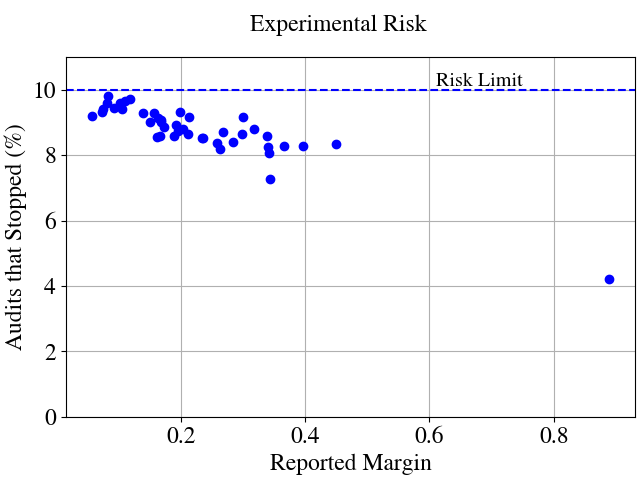
\includegraphics[width=.5\textwidth]{prov_risk.png}
\caption{The fraction of simulated \Providence audits on tied elections that stopped in any rounds (we performed five rounds at a $10\%$ risk limit). This value is an estimate of the maximum risk of the \Providence audit.}
\label{fig:prov-risk}
\end{figure}

In the simulations of \Providence audits of a tied election, the fraction of audits that stop, as shown in Figure~\ref{fig:prov-risk}, is an estimate of maximum risk. For all margins, this estimated maximum risk is less than the risk limit, supporting the claim that \Providence is risk-limiting.

\begin{figure}
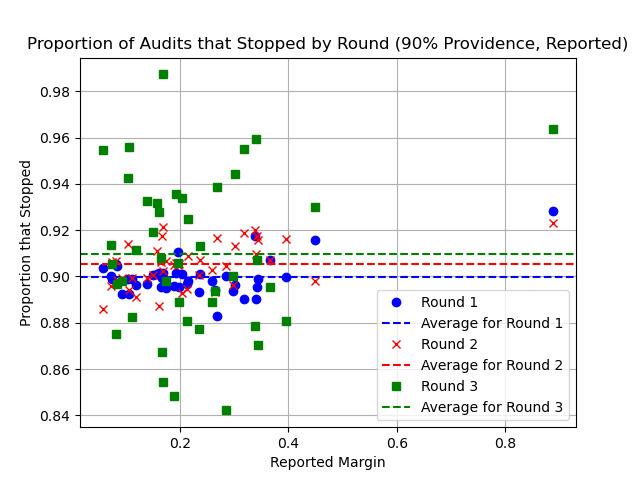
\includegraphics[width=.5\textwidth]{prov_sprob.png}
\caption{The fraction of simulated \Providence audits of the election as announced that stopped for each round. This value is an estimate of the stopping probability conditioned on the sample of the previous round. The average fraction for rounds 1, 2, and 3 is $89.96\%$, $90.52\%$, and $90.98\%$ respectively. We show only the first three rounds since so few audits make it to rounds 4 and 5.}
\label{fig:prov-sprob}
\end{figure}

Simulations of audits of the election as announced provide insight into stopping probability and number of ballots drawn when the election is as announced. We wish the stopping probability to be as predicted, and the number of ballots drawn to be small. Figure~\ref{fig:prov-sprob} shows that the stopping probabilities over the first rounds are near and slightly above $90\%$ as expected since our software chose round sizes to give at least a $90\%$ conditional stopping probability.

Figure~\ref{fig:prov-asn} plots the probability of stopping as a function of the number of ballots sampled. Points above (higher probability of stopping) and to the left (fewer ballots) represent more efficient audits. As shown, \Providence has comparable efficiency to \Minerva, while both are significantly more efficient than either implementation of \BRAVO. In a contest with a narrow margin (in the 2020 US Presidential election, eight states had margins less than $3\%$) the difference in number of ballots sampled could correspond to many days of work. 
% Section~\ref{sec:workload} discusses workload in more depth.

\begin{figure}
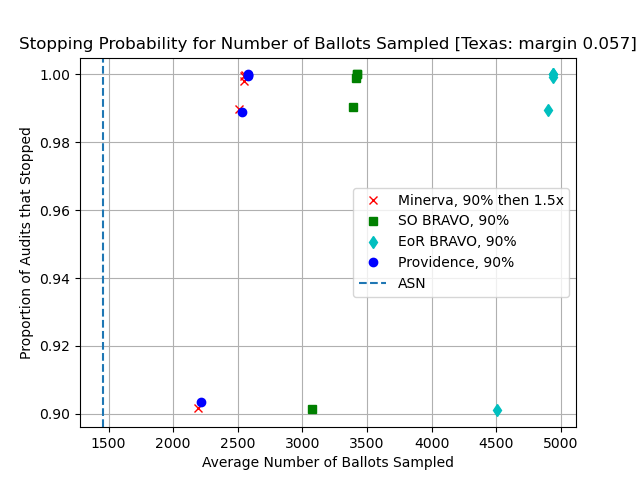
\includegraphics[width=.5\textwidth]{prov_asn.png}
\caption{For the entire audit, consisting of all five rounds, the estimated stopping probability for average number of ballots drawn for \Providence, \Minerva, EoR \BRAVO, and SO \BRAVO.}
\label{fig:prov-asn}
\end{figure}










\section{Pilot Use}
\label{sec:pilot}
% pilot
A pilot audit was performed in Providence, Rhode Island in February 2022 of November 2021 special elections.
The audited contest was a yes-or-no question on School Construction and Renovation Projects and had an announced $25.67\%$ margin.
The risk-limit was $10\%$.
A first round size of $140$ ballots with large probability of stopping ($95\%$) was selected, and selection order was tracked, in order to give the potential for more interesting analysis afterwards. 
As expected, the audit concluded in the first round with a \Providence risk of $4.18\%$. Table~\ref{tab:pilot-risks} shows risk measures for the drawn sample using \Minerva and \BRAVO (both EoR and SO).

\begin{table}
\begin{center}
\begin{tabular}{ |c|c|c|c|c| } 
\hline
%\diagbox[dir=NW]{First \\Round \\Size}{RLA}
ballots& \rotatebox{45}{\Providence} & \rotatebox{45}{\Minerva} & \rotatebox{45}{EoR \BRAVO} & \rotatebox{45}{SO \BRAVO} \\
\hline
140 & \bf{4.18\%} & \bf{4.18\%} & \bf{5.41\%} & 36.6\% \\
\hline
\end{tabular}
\end{center}
\caption{Risk measures for the drawn first round of $140$ ballots in the Providence, RI pilot audit. Risks in bold meet the risk-limit ($10\%$) and thus correspond to audits that would stop.}
\label{tab:pilot-risks}
\end{table}

TODO: Add examples of how the audits perform for various hypothetical round schedules. I wait to do this until I'm done with the workload estimates since the examples here should be chosen to motivate that section.


\section{Audit Workload}
\label{sec:workload}
Some election audits have benefited from a one-and-done approach: draw a large sample with high probability of stopping in the first round and usually avoid a second round altogether. This is appealing for two reasons. Firstly, rounds have some overhead in both time and effort. Thus the time and person-hours of an audit grows not just with the number of ballots sampled but also with the number of rounds. Secondly, smaller first round sizes are not large enough to accurately capture the distribution of votes. There is a higher probability that the true winner has fewer votes in the audit sample than some other candidate. On the other hand, a one-and-done audit may draw more ballots than are necessary; a more efficient round schedule could require less effort and time pre-certification. To evaluate the quality of various round schedules, we construct a simple workload model. Using this model we show how optimal round schedules can be chosen. We provide software that can be used by election officials to choose round schedules based on estimates of the model parameters like maximum allowed probability of a misleading audit sample.

As an example, we consider the US Presidential contest in the 2016 Virginia statewide general election. This contest had a margin of $0.053$ between the two candidates with the most votes.
Analytical approximation of the expected audit behavior (quantities like expected total number of ballots sampled or total number of rounds) is not straightforward. %challenging because the number of possible sequences of samples grows exponentially with the number of rounds. 
%A very rough approximation scheme is possible and may be useful when choosing round sizes in practice. We implement such a scheme, available at \cite{software}.
%We will use the more standard approach of simulations to give an example here.
Therefore we use the typical approach of simulations, again with risk limit $0.1$.

We simulate audits considering each candidate with a column in the results available at the Virginia Department of Elections website, including irrelevant ballots.
We consider a simple round schedule, in which each round is selected to give the same probability of stopping, $p$. That is, if the audit does not stop in the first round, we select a second round size which, given the sample drawn in the first round, will again have a probability of stopping $p$ in the second round. Note that since there are multiple candidates, we compute the minimum round size to achieve stopping probability $p$ for each pairwise contest between the winner and one of the losers, and we then select the largest such minimum round size and scale it up according to the proportion of the total ballots that are relevant to that pairwise contest. For this round schedule scheme, a one-and-done audit is achieved by choosing large $p$, say $p=.9$ or $p=.95$. We run $10^4$ trial audits for each value of $p$, assuming the reported results are correct\footnote{For this particular round schedule scheme, computing the expected number of rounds is straightforward analytically, but the expected number of ballots is still difficult, and so we use simulations.}. 

Note that simulations of audits of tied elections are not necessary, as all the audits we are considering are risk-limiting and hence we already know the performance to expect when auditing a tied election, even one not reported as such. 

Importantly, note that \Minerva does not appear in the analysis in this section. 
Questions about the efficiency of \Minerva for its necessarily fixed round schedules are addressed in section~\ref{sec:sims}, but in this section round sizes are chosen to have specified probabilities of stopping given previous samples. \Minerva is not known to be risk-limiting in this setting, and thus cannot be used for RLAs that proceed in this way.

\subsection{Person-hours}

\subsubsection{Average total ballots.} 
The simplest workload models are a function of just the total number of a ballots sampled\footnote{Sometimes total \emph{distinct} ballots sampled is used, but for the margins we use in our examples in this section, the difference between total distinct ballots and total ballots is very small\cite{arxiv_athena}. It is straightforward to modify the model we discuss here to account for total distinct ballots.}. Figure~\ref{fig:avg_bals} shows the average total number of ballots sampled as a function of $p$.
\begin{figure}[h!]
%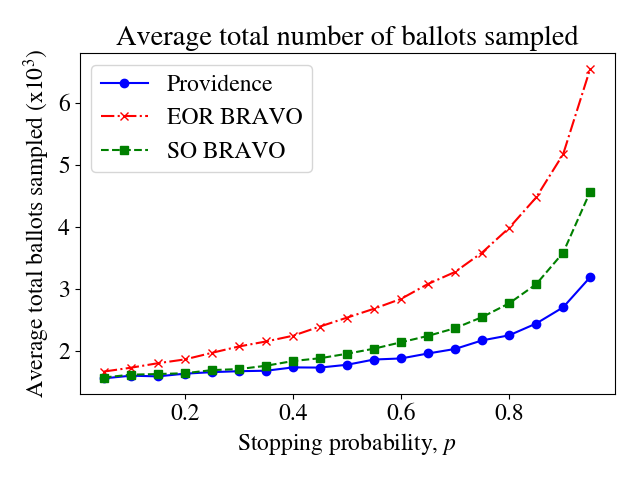
\includegraphics[width=.5\textwidth]{avg_bals.png}
%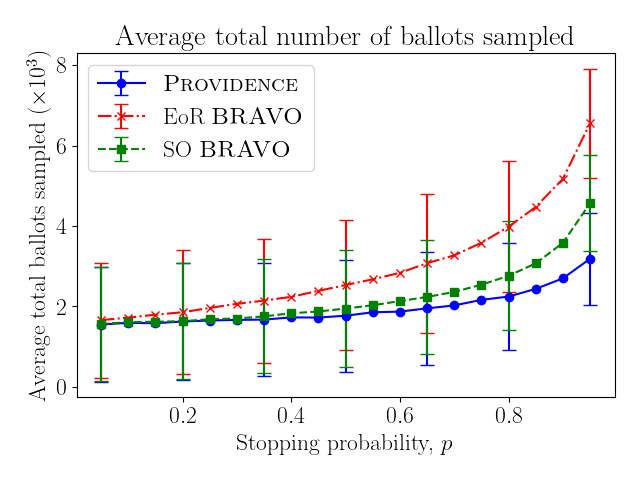
\includegraphics[width=.5\textwidth]{avg_bals_error_bars_every_three.png}
%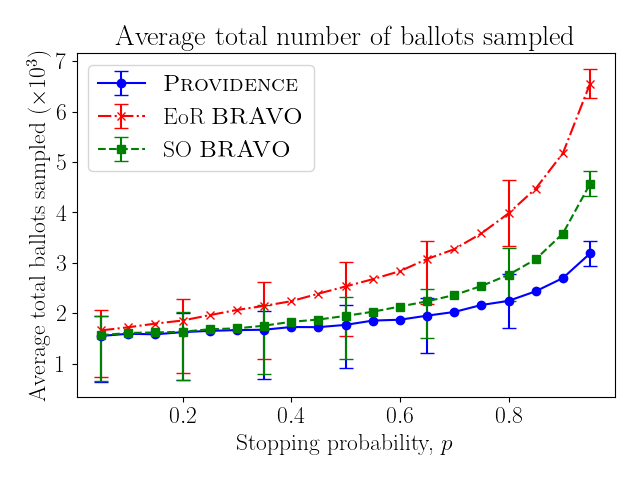
\includegraphics[width=.5\textwidth]{avg_bals_errorbars.png}
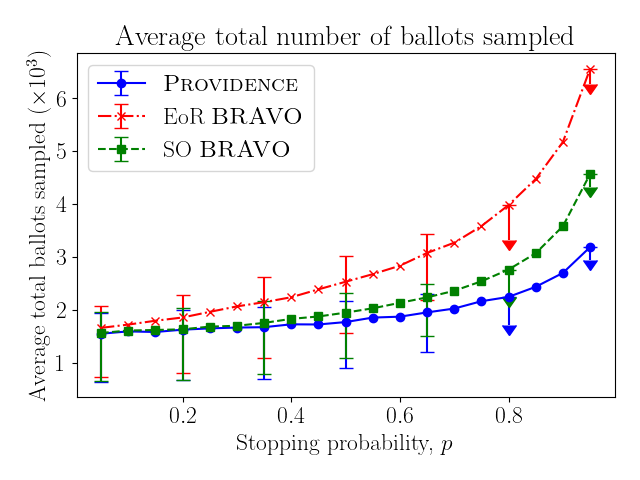
\includegraphics[width=.5\textwidth]{avg_bals_quantiles.png}
\caption{The average total number of ballots sampled, as a function of $p$, the conditional stopping probability used to select each round size, for ballot polling audits of the 2016 US Presidential election in the US State of Virginia. Error bars show the $0.25$ and $0.75$ quantiles. For sufficiently large $p$ ($p\ge 0.75$), the $0.25$ and $0.75$ quantiles are both equal to the first round size, and this is shown by the downward arrows.}
\label{fig:avg_bals}
\end{figure}

%Figure~\ref{fig:avg_bals_ratio} provides the same number as a fraction of the \Providence values.
It is straightforward to show that \Providence and both forms of \BRAVO collapse to the same test when each round corresponds to a single ballot. Figures~\ref{fig:avg_bals} 
%and \ref{fig:avg_bals_ratio} 
shows that for larger stopping probabilities $p$ (i.e. larger rounds), \Providence requires fewer ballots on average. In particular, the savings of \Providence become larger as $p$ increases; for $p=0.95$, EoR \BRAVO and SO \BRAVO require more than $2$ and $1.4$ times as many ballots as \Providence respectively. 

%\begin{figure}[h!]
%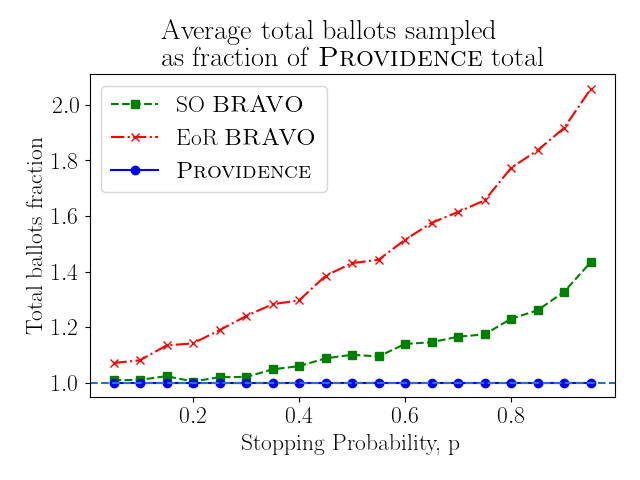
\includegraphics[width=.5\textwidth]{avg_bals_ratio.png}
%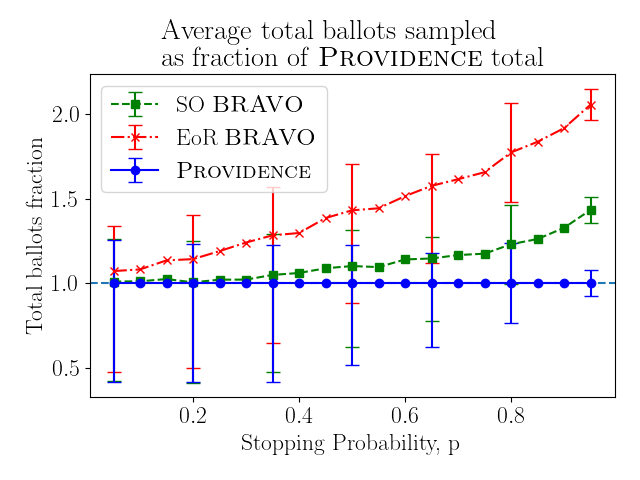
\includegraphics[width=.5\textwidth]{avg_bals_ratio_errorbars.png}
%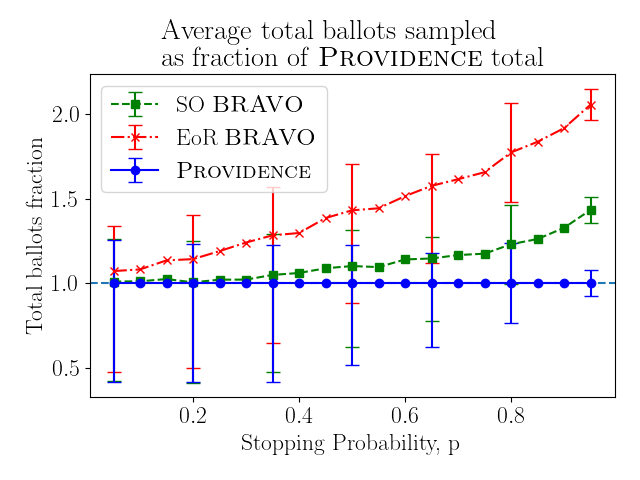
\includegraphics[width=.5\textwidth]{avg_bals_ratio_errorbars.png}
%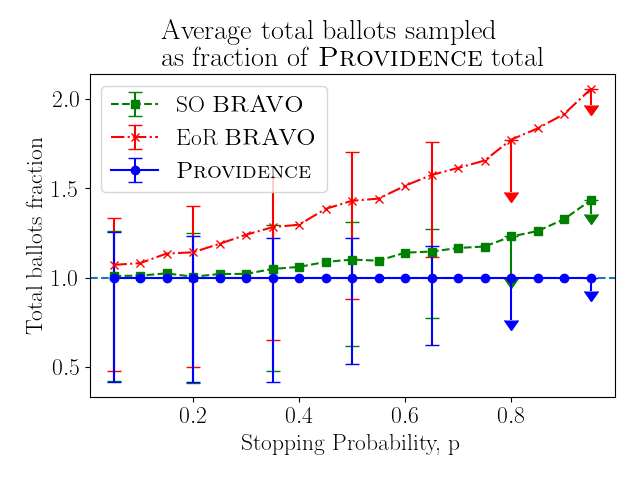
\includegraphics[width=.5\textwidth]{avg_bals_ratio_quantiles.png}
%\caption{The total number of ballots sampled on average, as a fraction of those sampled by \Providence, as a function of $p$, the conditional stopping probability used to select each round size, for ballot polling audits of the 2016 US Presidential election in the state of Virginia. The $0.25$ and $0.75$ quantiles are shown as in Figure~\ref{fig:avg_bals}.}
%\label{fig:avg_bals_ratio}
%\end{figure}


\subsubsection{Round overhead.} 
It is clear that average number of ballots alone is an inadequate workload measure. 
(Consider a state conducting its audit by selecting a single ballot at random, 
notifying just the county where the ballot is located, and then waiting to hear back for the manual interpretation of the ballot before moving on to the next one. 
This of course is inefficient and is why audits are actually performed in rounds.)

In a US state-wide RLA, the state organizes the audit by determining the random sample and communicating with the counties, but election officials at the county level physically sample and inspect the ballots after drawing them from secure storage boxes stored in county locations. 
Therefore each audit round requires some number of person-hours for set up and communication between state and county. This overhead for a round includes choosing the round size, generating the random sample, and communicating that random sample to the counties, as well as the communication of the results back to the state afterwards. 

Consequently, we now consider a model with a constant per-ballot workload $w_b$ and a constant per-round workload $w_r$.
So for an audit with expected number of ballots $E_{b}$ and expected number of rounds $E_{r}$, we estimate that the workload $W$ of the audit is
\begin{equation}
W(E_b,E_r) = E_b w_b + E_r w_r + C
\label{eq:round_workload}
\end{equation}

Note there is also some constant overhead of workload for the whole audit, namely $C$ in Equation~\ref{eq:round_workload}, which we take to be zero in our examples but could be used by election officials to represent, for example, the effort of constructing a ballot manifest.
For simplicity, (and without loss of generality), we measure in multiples of the per ballot workload; that is, we assume it is one unit, $w_b=1$. A per round workload of $w_r=x$ corresponds to a per round workload which is $x$ times the per ballot workload. We use $w_r=1000$ as a conservative example. 
That is, we set the overhead of a round equal to the workload of sampling $1000$ ballots. Based on available data\cite{RI-report}, the time retrieving and analyzing each individual ballot is on the order of $75$ seconds which means that $w_r=1000$ is equivalent to roughly $20$ person-hours of workload. This corresponds to about $15$ minutes being spent, on average, per round in each of the $133$ counties of Virginia, a clearly conservative workload estimate. We do not consider $w_r < 1$ because it is not possible for the round overhead to be smaller than the workload corresponding to a single ballot. 

As shown in Figure~\ref{fig:with_round_workload}, average workloads first reduce as stopping probability increases; this is likely due to a decrease in the number of rounds. After hitting a sweet spot, average workloads again increase with stopping probability; this time, likely because the average number of rounds does not decrease much and the cost changes because of number of ballots drawn, which increases with round size. \Providence achieves the lowest minimum average workload at roughly $p=0.7$ for our example choice of $w_r=1000$.

\begin{figure}[h!]
%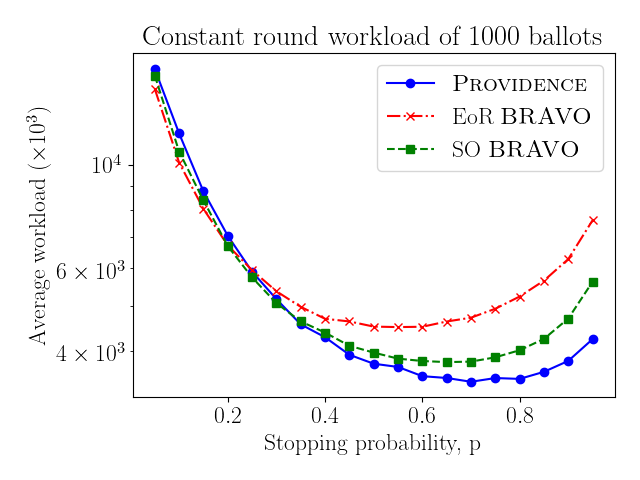
\includegraphics[width=.5\textwidth]{with_round_workload.png}
%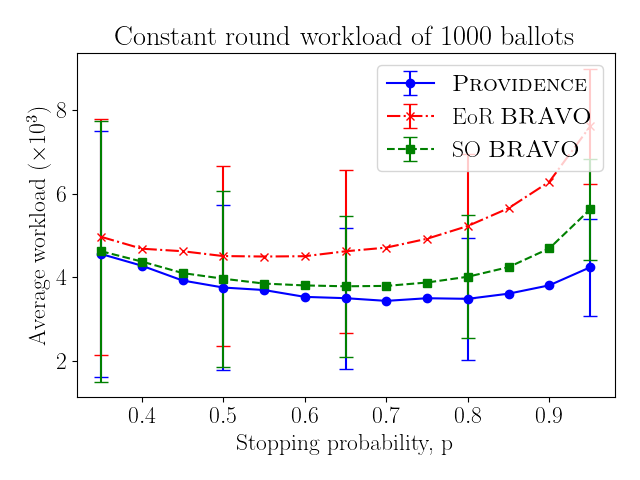
\includegraphics[width=.5\textwidth]{with_round_workload_errorbars.png}
%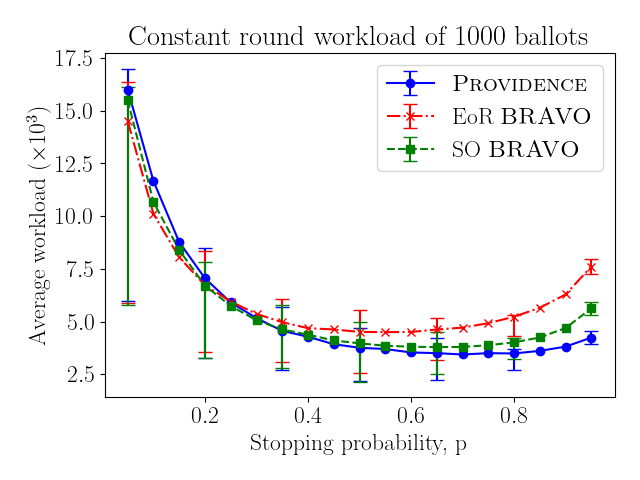
\includegraphics[width=.5\textwidth]{round_workload_errorbars.png}
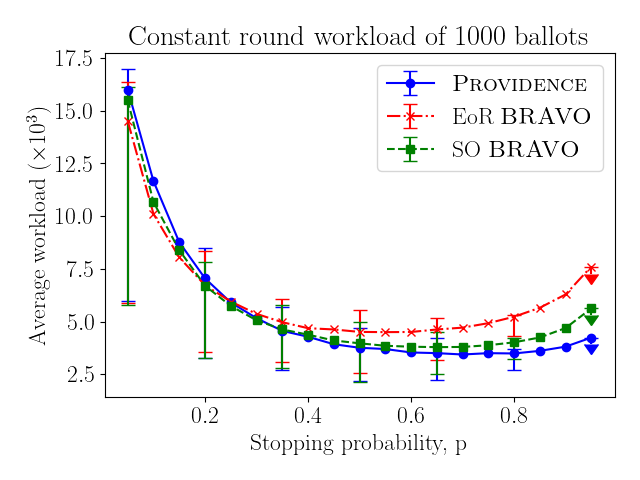
\includegraphics[width=.5\textwidth]{round_workload_quantiles.png}
\caption{For workload parameters $w_b=1$ and $w_r=1000$, this plot shows the expected workload for various values of $p$. Expected workload is found using Equation~\ref{eq:round_workload} and the average number of ballots and rounds in our simulations as the expected number of ballots and rounds. The $0.25$ and $0.75$ quantiles are shown as in Figure~\ref{fig:avg_bals}.}
\label{fig:with_round_workload}
\end{figure}

Importantly, this gives us a way to estimate the minimum expected workload, as well as which round schedule value $p$ achieves it, for arbitrary round workload. For each round workload $w_r$, we produce a dataset analagous to that of Figure~\ref{fig:with_round_workload} and then find the minimum average workload achieved for each of the audits and its corresponding stopping probability $p$. 

Figure~\ref{fig:optimal_workloads} shows the optimal achievable workload for a wide range of per round workloads. For very low round workloads, the workload function approaches just the total number of ballots, and so workload is minimized by minimizing the number of ballots drawn, which corresponds to small round sizes, and we would expect all three audits to behave similarly, as ballot-by-ballot audits, with the smallest workload. On the other hand, for extremely large values of round workload, the average number of ballots has little impact on the workload function, and so the three audits again have similar values, all corresponding to large round sizes in order to minimize the number of rounds.  We know that there is variation in the number of ballots used by each type of audit for large round sizes (a factor of two for $p=0.9$), but these values would be small in comparison to $w_r$. We observe this behaviour in Figure~\ref{fig:optimal_workloads} for extremely small and large workload values. For more reasonable values of the round workload $w_r$, SO \BRAVO and EoR \BRAVO achieve minimum workload roughly $1.1$ and $1.3$ times greater than that of \Providence.
\begin{figure}[h!]
%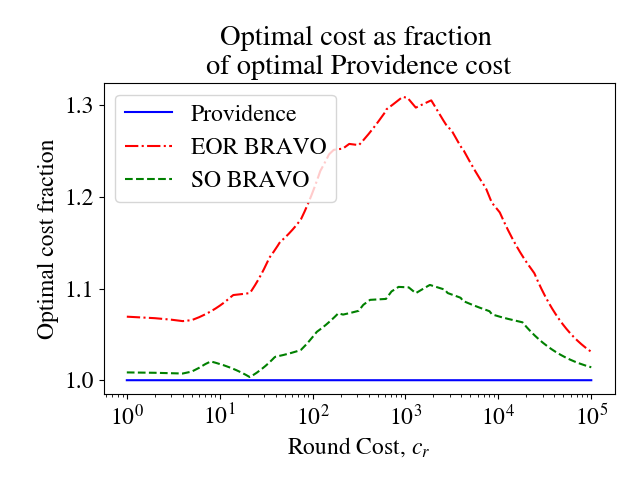
\includegraphics[width=.5\textwidth]{optimal_workloads.png}
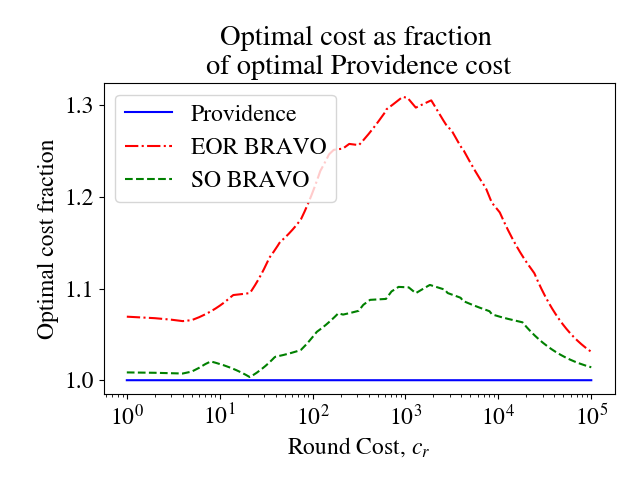
\includegraphics[width=.5\textwidth]{optimal_workloads.png}
\caption{For varying round workload $w_r$, the optimal average workload achievable by each audit, as a fraction of the \Providence values.}
\label{fig:optimal_workloads}
\end{figure}

Figure~\ref{fig:optimal_ps} shows the corresponding round schedule parameters $p$ that achieve these minimal workloads. As expected, an overhead for each round means that larger round sizes are needed to achieve an optimal audit, and so for all three audits $p$ increases as a function of $w_r$. Notice that \Providence is generally above and to the left of SO \BRAVO, and SO \BRAVO is generally above and to the left of EoR \BRAVO. This relationship reflects the fact that for the same round workload, \Providence can get away with a larger stopping probability because it requires fewer ballots.
\begin{figure}[h!]
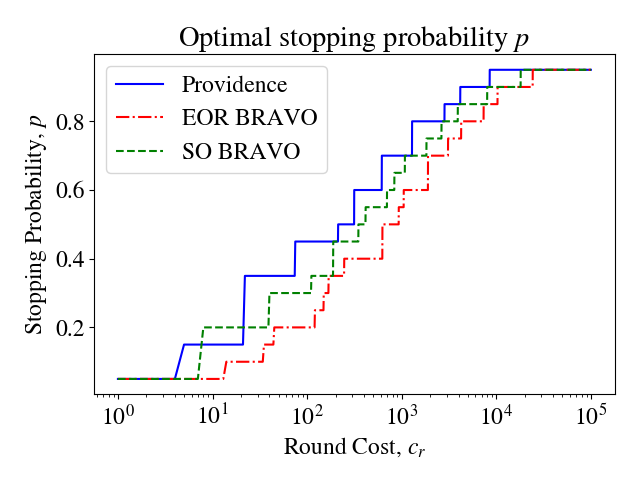
\includegraphics[width=.5\textwidth]{optimal_ps.png}
\caption{The optimal (workload-minimizing) stopping probability $p$ for varying workload model parameters $w_r$. (Note that the steps in this function are a consequence of our subsampling the workload function. That is, the workload-minimizing value of $p$ for each $w_r$ is only allowed to take on values at increments of $0.05$.)}
\label{fig:optimal_ps}
\end{figure}

\subsubsection{Precinct overhead.} For a more complete model, we can also introduce container-level workload. If a round requires multiple ballots from a single container, the container need only be unsealed once. Based on a Rhode Island pilot RLA report\cite{RI-report}, this may mean that a ballot from a new container requires roughly twice the time as a ballot from an already-opened container. Typically available election results give per-precinct granularity of vote tallies, rather than individual container information. In Virginia, however, most precincts have a single ballot scanner whose one box has sufficient capacity for all the ballots cast in that precinct anyways, and so we model the per-container workload as a per-precinct workload, $w_p$. In this model, the workload estimate incurs an additional workload of $w_p$ every time a precinct is sampled from for the first time in a round. That is, let $E_{pi}$ be the expected number of distinct precincts sampled from in round $i$, and let $E_p=\sum_i E_{pi}$. Then the new model is
\begin{equation}
W(E_b, E_r, E_p) = E_b w_b + E_r w_r + E_p w_p + C
\label{eq:round_and_precinct_workload}
\end{equation}

We can again explore the minimum achievable workloads under this model, as shown in Figure~\ref{fig:optimal_workload_precinct_workload_ratio}.

\begin{figure}
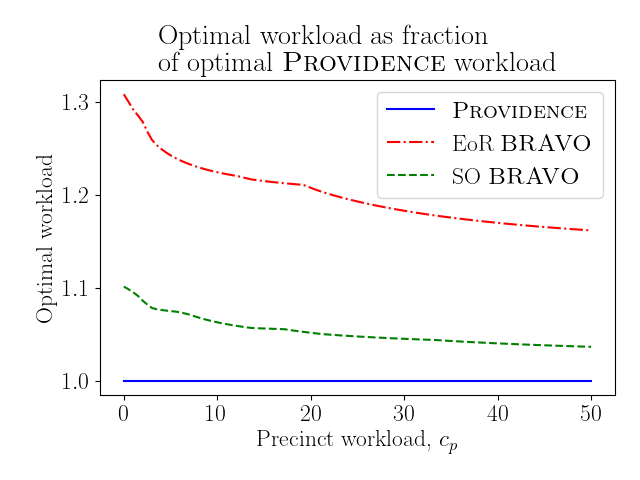
\includegraphics[width=.5\textwidth]{optimal_workload_precinct_workload_ratio.png}
\caption{Optimal average workload using the workload Equation~\ref{eq:round_and_precinct_workload} for varying $w_p$, given as a fraction of the value for \Providence. Similar to Figure~\ref{fig:optimal_workloads}, we show a generous range of values for the workload variable, $c_p$ in this case. If the time for a single ballot is $75$ seconds, then $c_p=50$ corresponds to over an hour of extra time to sample a ballot from a new container.}
\label{fig:optimal_workload_precinct_workload_ratio}
\end{figure}


\subsection{Real time}
Given tight certification deadlines,
%\footnote{Virginia recently passed legislation requiring pre-certification RLAs.}, 
the total real time to conduct the RLA is also an important factor to consider when planning audits.
Because each county can sample ballots for the same round concurrently, the total real time for a round depends only on the slowest county. 
In Virginia, Fairfax County typically has the most votes cast by a significant difference; in the contest we consider, Fairfax County had ~551 thousand votes cast, more than double the ~203 thousand of second-highest Virginia Beach City.
Consequently, we model the expected total real time $T$ of an audit using just the largest county, and we define analagous variables for the expected values in just the largest county.
Note that some other county may be slower, having fewer votes but also less auditing resources; but still, a slowest county exists. In this example, we take it to be Fairfax, the largest.
For the slowest county, let the expected total ballots sampled be $\bar E_b$, the expected number of rounds $\bar E_r$, and the expected number of distinct precinct samples summed over all rounds be $\bar E_p$.
Similarly, we use real time per-ballot, per-round, and per-precinct workload variables, $t_b$, $t_r$, and $t_p$. So the real time of the audit is estimated by
\begin{equation}
T(\bar E_b, \bar E_r, \bar E_p ) = \bar E_b t_b + \bar E_r t_r + \bar E_p t_p + C
\label{eq:real_time}
\end{equation}

As before, we can use our simulations to estimate $\bar E_b$, $\bar E_r$, and $\bar E_p$ using the corresponding averages over the trials. 
Available data to estimate values for $t_b$, $t_r$, and $t_p$ is limited, and so we take as an example the values $t_b=75$ seconds, $t_r=3$ hours, and $t_p=75$ seconds\footnote{The value $t_b=75$ seconds corresponds to a serial retrieval and interpretation of the ballots based on the \cite{RI-report} timing, $t_p=75$ seconds corresponds to the approximate doubling in time for new-box ballots as reported in \cite{RI-report} in the ballot-level comparison timing data, and $t_r=3$ hours is just a guess at an approximate order of magnitude for this variable.}. In practice, election officials could use our software and their own estimates of these values to explore choices for round schedules. Figure~\ref{fig:real_time} shows how the estimated real time for these values differs as a function of $p$. It should be noted that real values of $t_b$, $t_r$, and $t_p$ will vary greatly based on the number of parallel teams retrieving and checking ballots, the distribution of ballots and containers both in number and physical space, and other factors. We provide Figure~\ref{fig:real_time} only as an example of the general shape and behavior of this function. Use of this optimal scheduling tool would depend on parameter estimates tailored to each case.

\begin{figure}
%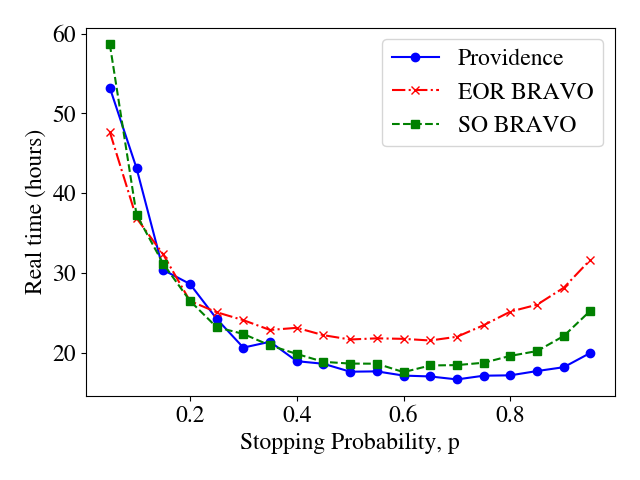
\includegraphics[width=.5\textwidth]{real_time.png}
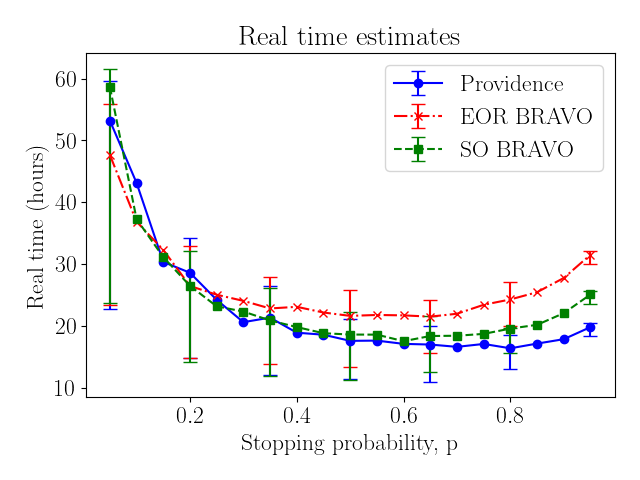
\includegraphics[width=.5\textwidth]{real_time_errorbars.png}
\caption{The real time as estimated by Equation~\ref{eq:real_time} for varying $p$ with expected values as estimated by our simulations. Error bars show the $0.25$ and $0.75$ quantiles. Unlike Figures \ref{fig:avg_bals}, \ref{fig:avg_bals_ratio}, and \ref{fig:with_round_workload}, the quantiles still differ for large $p$ because the first round size is no longer a constant; the number of ballots drawn in the first round in Fairfax County is variable.}
\label{fig:real_time}
\end{figure}


\section{Misleading samples}
\label{sec:misleading}

Unfortunately, efficiency alone is not sufficient for planning audits. In the US today, election officials have a legitimate need to include personal safety as a consideration.
In a random sample, a true loser may receive more votes than the true winner. This happens more often when the sample sizes are small, like for a hypothetical first round size of $11$ in the pilot audit, as seen in Figure~\ref{fig:pilot_sequence}.
In the abstract, a misleading sample in an early round is dealt with by drawing more ballots (moving on to another round), but in practice it serves to create expectations or suspicions that then need to be managed by election officials. Hence there is reason to structure round sizes so that they are unlikely to misrepresent the true outcome.

%, angry supporters of the losing candidate may be suspicious of election officials moving onto a next round, or, if the audit is declared correct after the second round, feel sufficiently disappointed to pose a threat. 
%but in practice the implications of this approach may be dangerous.

%Imagine that Alice beats Bob in an election contest both truly and in the reported results, but Bob's supporters are insistent he really won. When election officials carry out the RLA, they choose a small first round size in the hopes of achieving an efficient audit by getting to stop sooner (and drawing fewer ballots on average). 
% After the first round, by chance, there are more votes for Bob than for Alice in the sample. Bob's supporters celebrate their victory that the audit has in fact revealed that Bob really won, but the election officials have to explain that they are moving on to a second round. 

%After the second round, there are more votes in the sample for Alice and sufficiently many that the risk limit is met and the audit now ends confirming the announced result that Alice won. This is an undesirable situation, as it can appear to Bob's supporters that election officials are simply drawing ballots till a chosen outcome is obtained. 

We introduce the notion of a \emph{misleading sample}, any cumulative sample which, assuming the announced outcome is correct, contains more ballots for a loser than for the winner.
We can again use our simulations to gain insight into the frequency of \emph{misleading samples}.
For each stopping probability $p$, Figure~\ref{fig:misleading} gives the proportion of simulated audits that had a \emph{misleading sample} at any point. 
Notably, this proportion is as high as 1 in 5 for the smaller stopping probability round schedules.
Accordingly, we introduce a new parameter to our audit-planning tool, the maximum acceptable probability that the audit is misleading, the \emph{misleading limit}.

In Figure~\ref{fig:misleading}, horizontal lines are included to show \emph{misleading limits} of $0.1$, $0.01$, and $0.001$.
To achieve a probability of a misleading sample of at most $0.1$, a round schedule with at least roughly $p=.3$ is needed.
To achieve a probability of misleading of roughly $0.01$, a round schedule with $p=0.8$ is needed, and to achieve a probability of misleading of roughly $0.001$, a round schedule with $p=0.95$ is needed.
It is not unreasonable to think that election officials might choose a \emph{misleading limit} of $0.01$, or smaller, given the state of public perception of election security in the US and the associated threats of violence.
Consequently, the desired \emph{misleading limit} may be a deciding constraint in the choice of round schedule. 

\begin{figure}
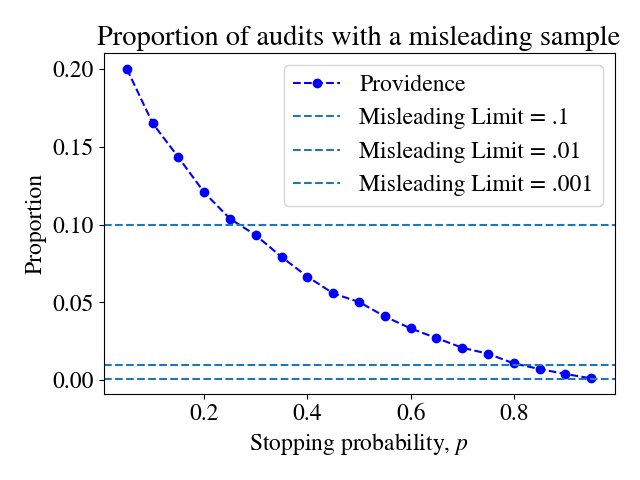
\includegraphics[width=.5\textwidth]{misleading_limits.png}
%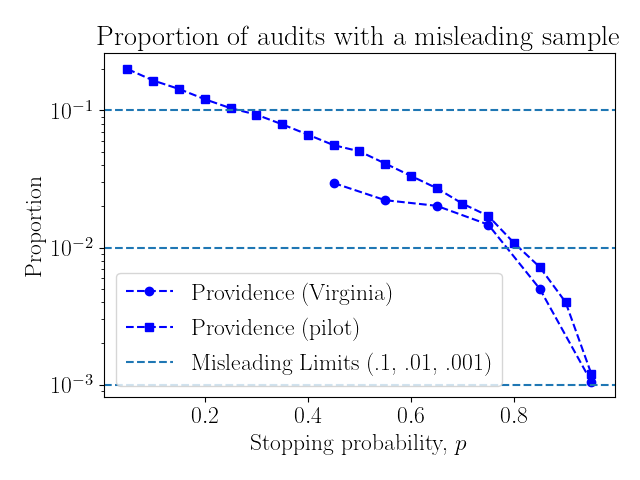
\includegraphics[width=.5\textwidth]{combined_misleading.png}
\caption{The proportion of simulated \Providence audits for the Virginia and pilot contest parameters that had a \emph{misleading sample} in any round.}
\label{fig:misleading}
\end{figure}

%We observe a similar behavior in our simulations of audits on the contest from the pilot audit. Figure~\ref{fig:misleading} also shows the proportion of the pilot simulations which contained a \emph{misleading sample} in any round. Despite the large difference in margin ($\sim 0.05$ in Virginia and $\sim 0.25$ in the pilot) we still observe that a \emph{misleading limit} of $0.01$ is first achieved at roughly $p=0.8$ and $0.001$ at $p=0.95$.

%\begin{figure}
%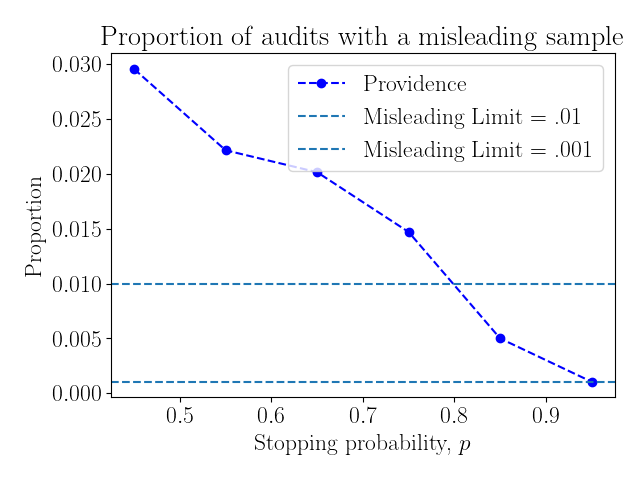
\includegraphics[width=.5\textwidth]{pilot_misleading_prop.png}
%\caption{The proportion of simulated \Providence audits for the pilot audit parameters that had a \emph{misleading sample} in any round.}
%\label{fig:pilot_misleading}
%\end{figure}

If election officials wish to enforce a \emph{misleading limit} for all the rounds, our simulation analysis could help. On the other hand, for a given round, it is straightforward to compute analytically the probability that a loser has more votes than the winner in the sample. Table~\ref{tab:misleading} shows for various margins the minimum first round size $n$ that guarantees a probability of a \emph{misleading sample} at most $M\in\{0.1,0.01,0.001\}$. For all values of $M$ and all margins, \Providence achieves a higher probability of stopping than either EoR \BRAVO or SO \BRAVO. 
    As seen in the Table~\ref{tab:misleading}, to enforce $M=0.01$ requires minimum round sizes with at least roughly a $0.8$ probability of stopping in the first round. Even if the most efficient audit schedule (by either workload or real time measures) would use a lower stopping probability $p$ to choose the first round size, the election officials may opt to use this constraint on the probability of a \emph{misleading sample} as the deciding factor in planning their audits.

\section{Conclusion}
\label{sec:conc}
%Conclusions
A rigorous tabulation audit is an important part of a secure election. Ballot polling RLAs are commonly used and simple, not relying on special election equipment like comparison RLAs. We present \Providence which is the most efficient and secure ballot polling RLA, as efficient as \Minerva  and flexible as \BRAVO. We present proofs and simulation results to verify the claimed properties of \Providence, and we provide an open source implementation of the stopping condition and useful related functionality.


\begin{table}[h!]
\center
\begin{tabular}{ |l|l|r|c|c|c| }
\hline
$M$ & margin & $n$ & Prov & SO & EoR \\
\hline
0.1&0.25&25&0.221&0.152&0.115\\
%&0.2&41&0.178&0.169&0.105\\
&0.15&73&0.202&0.186&0.141\\
%&0.1&163&0.222&0.182&0.107\\
&0.05&657&0.227&0.192&0.127\\
%&0.04&1027&0.237&0.193&0.124\\
&0.03&1825&0.246&0.194&0.124\\
%&0.02&4105&0.246&0.195&0.124\\
&0.01&16423&0.246&0.196&0.124\\
\hline
0.01&0.25&85&0.792&0.707&0.559\\
%&0.2&133&0.826&0.71&0.593\\
&0.15&239&0.817&0.712&0.549\\
%&0.1&539&0.805&0.717&0.567\\
&0.05&2163&0.817&0.721&0.569\\
%&0.04&3381&0.82&0.722&0.563\\
&0.03&6011&0.824&0.723&0.573\\
%&0.02&13527&0.824&0.723&0.57\\
&0.01&54117&0.824&0.724&0.57\\
\hline
0.001&0.25&149&0.962&0.889&0.783\\
%&0.2&235&0.963&0.89&0.768\\
&0.15&421&0.958&0.894&0.801\\
%&0.1&951&0.958&0.894&0.793\\
&0.05&3815&0.96&0.896&0.785\\
%&0.04&5965&0.961&0.896&0.791\\
&0.03&10607&0.961&0.897&0.787\\
%&0.02&23869&0.962&0.897&0.787\\
&0.01&95491&0.962&0.897&0.787\\
\hline
\end{tabular}
\caption{For various margins, this table gives the minimum first round size $n$ to achieve at most a probability $M$ of a \emph{misleading sample} in the first round. The corresponding stopping probabilities of \Providence, SO \BRAVO, and EoR \BRAVO are given for each value of $n$.}
\label{tab:misleading}
\end{table}



\section{Availability}
\label{sec:avail}
\Providence is implemented in the open source R2B2 software library for \R and \B audits \cite{r2b2_anon} 
% The software library includes implementations of SO and EoR \BRAVO also. 
We provide software to test stopping conditions, find round sizes to achieve a given probability of stopping, and find round sizes that have acceptable probabilities of a \emph{misleading sample}. The software also includes the simulator for all these audits and the functionality to perform the workload and real time analysis we present in this paper.

\section{Acknowledgements}
\label{sec:ack}
The authors are grateful to the Rhode Island Board of Elections for conducting a pilot \Providence RLA, and to Georgina Cannan, Liz Howard, Mark Lindeman, and John Marion for their support of the pilot.  The authors thank Audrey Malagon for useful information on audits.

% The authors thank Georgina Cannan for insightful comments.


%-------------------------------------------------------------------------------
%\section{Introduction}
%%-------------------------------------------------------------------------------
%
%A paragraph of text goes here. Lots of text. Plenty of interesting
%text. Text text text text text text text text text text text text text
%text text text text text text text text text text text text text text
%text text text text text text text text text text text text text text
%text text text text text text text.
%More fascinating text. Features galore, plethora of promises.
%
%%-------------------------------------------------------------------------------
%\section{Footnotes, Verbatim, and Citations}
%%-------------------------------------------------------------------------------
%
%Footnotes should be places after punctuation characters, without any
%spaces between said characters and footnotes, like so.%
%\footnote{Remember that USENIX format stopped using endnotes and is
%  now using regular footnotes.} And some embedded literal code may
%look as follows.
%
%\begin{verbatim}
%int main(int argc, char *argv[]) 
%{
%    return 0;
%}
%\end{verbatim}
%
%Now we're going to cite somebody. Watch for the cite tag. Here it
%comes. Arpachi-Dusseau and Arpachi-Dusseau co-authored an excellent OS
%book, which is also really funny~\cite{arpachiDusseau18:osbook}, and
%Waldspurger got into the SIGOPS hall-of-fame due to his seminal paper
%about resource management in the ESX hypervisor~\cite{waldspurger02}.
%
%The tilde character (\~{}) in the tex source means a non-breaking
%space. This way, your reference will always be attached to the word
%that preceded it, instead of going to the next line.
%
%And the 'cite' package sorts your citations by their numerical order
%of the corresponding references at the end of the paper, ridding you
%from the need to notice that, e.g, ``Waldspurger'' appears after
%``Arpachi-Dusseau'' when sorting references
%alphabetically~\cite{waldspurger02,arpachiDusseau18:osbook}. 
%%
%It'd be nice and thoughtful of you to include a suitable link in each
%and every bibtex entry that you use in your submission, to allow
%reviewers (and other readers) to easily get to the cited work, as is
%done in all entries found in the References section of this document.
%
%Now we're going take a look at Section~\ref{sec:figs}, but not before
%observing that refs to sections and citations and such are colored and
%clickable in the PDF because of the packages we've included.
%
%%-------------------------------------------------------------------------------
%\section{Floating Figures and Lists}
%\label{sec:figs}
%%-------------------------------------------------------------------------------
%
%
%%---------------------------
%\begin{figure}
%\begin{center}
%\begin{tikzpicture}
%  \draw[thin,gray!40] (-2,-2) grid (2,2);
%  \draw[<->] (-2,0)--(2,0) node[right]{$x$};
%  \draw[<->] (0,-2)--(0,2) node[above]{$y$};
%  \draw[line width=2pt,blue,-stealth](0,0)--(1,1)
%        node[anchor=south west]{$\boldsymbol{u}$};
%  \draw[line width=2pt,red,-stealth](0,0)--(-1,-1)
%        node[anchor=north east]{$\boldsymbol{-u}$};
%\end{tikzpicture}
%\end{center}
%\caption{\label{fig:vectors} Text size inside figure should be as big as
%  caption's text. Text size inside figure should be as big as
%  caption's text. Text size inside figure should be as big as
%  caption's text. Text size inside figure should be as big as
%  caption's text. Text size inside figure should be as big as
%  caption's text. }
%\end{figure}
%%% %---------------------------
%
%
%Here's a typical reference to a floating figure:
%Figure~\ref{fig:vectors}. Floats should usually be placed where latex
%wants then. Figure\ref{fig:vectors} is centered, and has a caption
%that instructs you to make sure that the size of the text within the
%figures that you use is as big as (or bigger than) the size of the
%text in the caption of the figures. Please do. Really.
%
%In our case, we've explicitly drawn the figure inlined in latex, to
%allow this tex file to cleanly compile. But usually, your figures will
%reside in some file.pdf, and you'd include them in your document
%with, say, \textbackslash{}includegraphics.
%
%Lists are sometimes quite handy. If you want to itemize things, feel
%free:
%
%\begin{description}
%  
%\item[fread] a function that reads from a \texttt{stream} into the
%  array \texttt{ptr} at most \texttt{nobj} objects of size
%  \texttt{size}, returning returns the number of objects read.
%
%\item[Fred] a person's name, e.g., there once was a dude named Fred
%%%  who separated usenix.sty from this file to allow for easy
%%  inclusion.
%%\end{description}
%%
%%\noindent
%%The noindent at the start of this paragraph in its tex version makes
%it clear that it's a continuation of the preceding paragraph, as
%opposed to a new paragraph in its own right.
%
%
%\subsection{LaTeX-ing Your TeX File}
%%-----------------------------------
%
%People often use \texttt{pdflatex} these days for creating pdf-s from
%tex files via the shell. And \texttt{bibtex}, of course. Works for us.
%
%%-------------------------------------------------------------------------------
%\section*{Acknowledgments}
%%-------------------------------------------------------------------------------
%
%The USENIX latex style is old and very tired, which is why
%there's no \textbackslash{}acks command for you to use when
%acknowledging. Sorry.
%
%%-------------------------------------------------------------------------------


%%-------------------------------------------------------------------------------
%
%USENIX program committees give extra points to submissions that are
%backed by artifacts that are publicly available. If you made your code
%or data available, it's worth mentioning this fact in a dedicated
%section.
%
%-------------------------------------------------------------------------------
\bibliographystyle{plain}
\bibliography{audits.bib}




%appendix:

\appendix

\section{Proofs}
\label{sec:proofs}
\begin{lemma}
    \label{lemma:sigma_increasing}
For $0<p_0< p_a< 1$ and $n>0$, the ratio $\sigma(k,p_a,p_0,n)$ is strictly increasing as a function of $k$ for $0\le k\le n$.
\end{lemma}
\begin{proof}
See \cite[Lemma 4]{usenix_minerva}. 
\end{proof}

\begin{lemma}
    \label{lemma:frac_sums_increasing}
    Given a monotone increasing sequence: $\frac{a_1}{b_1}, \frac{a_2}{b_2}, \ldots, \frac{a_n}{b_n}$, for $a_i, b_i > 0$, the sequence:
    $$z_i = \frac{\sum_{j=i}^n a_j}{\sum_{j=i}^n b_j}$$
    is also monotone increasing.
\end{lemma}

\begin{proof}
See \cite[Lemma 2]{usenix_minerva}. 
\end{proof}

\begin{lemma}
    \label{lemma:tau1_increasing}
For $0<p_0< p_a< 1$ and $n>0$, the ratio $\tau_1(k,p_a,p_0,n)$ is strictly increasing as a function of $k$ for $0\le k\le n$.
\end{lemma}
\begin{proof}
    Apply Lemmas \ref{lemma:sigma_increasing}-\ref{lemma:frac_sums_increasing}.
\end{proof}
\begin{lemma}
    \label{lemma:imin-exists}
    Given a strictly monotone increasing sequence: $x_1, x_2, \ldots x_n $ and some constant $A$,
    %there exists an $i_{min}$ such that
    $$A \le x_i \Leftrightarrow \exists i_{min} \le i ~\text{s.t.}~   x_{i_{min} -1} < A \le x_{i_{min}} \le x_{i},$$
    unless $A\le x_1$, in which case $i_{min} =1 $.
\end{lemma}
\begin{proof}
    Evident.
\end{proof}

\begin{lemma}
    \label{lemma:minerva2_kmin_exists}
    For $\mathcal{A}=(\alpha,p_a, p_0,k_{j-1},n_{j-1},n_j)$-\Providence, there exists\\ a 
    $k^{p_a, p_0, \alpha, k_{j-1}}_{min, j, n_{j-1}, n_j}  = 
    k_{min,j}(\Providence, p_a, p_0, k_{j-1}, n_{j-1}, n_j)$ such that $$\mathcal{A}(X_j)=\text{Correct}\iff k_j\ge k_{min,j}(\Providence,  \bm{n_j}, p_a, p_0).$$
\end{lemma}
\begin{proof}
    From Definition~\ref{def:minervatwo}, $$\mathcal{A}(X_j)=\text{Correct}\iff \omega_j(k_{j}, k_{j-1}, p_a, p_0, n_j, n_{j-1}) \ge \frac{1}{\alpha}.$$
    Now to apply Lemma~\ref{lemma:imin-exists}, it suffices to show that
    $\omega_j$ is monotone increasing with respect to $k_j$.
    For $j=1$, we have $\omega_1=\tau_1$, so $\omega_1$ is strictly increasing by Lemma \ref{lemma:tau1_increasing}. For $j\ge 2$,
    $$\omega_j(k_j,k_{j-1},p_a,p_0,n_j,n_{j-1},\alpha)=$$$$\sigma(k_{j-1},p_a,p_0,n_{j-1})\cdot \tau_1(k_{j}-k_{j-1},p_a,p_0,n_j-n_{j-1}).$$
    As a function of $k_j$, $\sigma$ is constant, and thus $\omega$ is strictly increasing by Lemma \ref{lemma:tau1_increasing}. Therefore by Lemma \ref{lemma:imin-exists}, we have the desired property.
\end{proof}

\begin{lemma}
\label{lemma:any_ratio_is_sigma_simple}
For $j\ge 1$,
$$\frac{Pr[\bm{K_j}=\bm{k_j} \mid \bm{n_j}, H_a]}{Pr[\bm{K_j}=\bm{k_j} \mid \bm{n_j}, H_0]} = \sigma(k_j, p_a, p_0, n_j).$$
\end{lemma}
\begin{proof}
We induct on the number of rounds.
For $j=1$, we have
$$\frac{Pr[\bm{K_1}=\bm{k_1} \mid \bm{n_1},H_a]}{Pr[\bm{K_1}=\bm{k_1} \mid  \bm{n_1},H_0]} =\frac{Pr[K_1 = k_{1} \mid n_1,H_a]}{Pr[K_1 = k_1 \mid n_1,H_0]} $$$$= \frac{\text{Bin}(k_1,n_1,p_a)}{\text{Bin}(k_1,n_1,p_0)}=\sigma(k_1, p_a, p_0, n_1).$$
Suppose the lemma is true for round $j=m$ with history $\bm{k_m}$.
Observe that
 $$\frac{Pr[\bm{K_{m+1}}=\bm{k_{m+1}} \mid \bm{n_{m+1}},H_a]}{Pr[\bm{K_{m+1}}=\bm{k_{m+1}} \mid \bm{n_{m+1}}, H_0]} $$$$= \frac{ Pr[\bm{K_{m}}=\bm{k_{m}}\mid \bm{n_{m+1}},H_a] \cdot Pr[K_{m+1}'=k_{m+1}'|\bm{k_m},\bm{n_{m+1}},H_a]}{ Pr[\bm{K_{m}}= \bm{k_{m}} \mid  \bm{n_{m+1}},H_0]  \cdot  Pr[K_{m+1}'=k_{m+1}'|\bm{k_m},\bm{n_{m+1}},H_0]  }$$
 $$=\sigma(k_m, p_a, p_0, n_m) \cdot \frac{Pr[K_{m+1}'=k_{m+1}'|\bm{k_m}, \bm{n_{m+1}}, H_a]}{Pr[K_{m+1}'=k_{m+1}'|\bm{k_m},\bm{n_{m+1}},H_0]}$$
 by the induction hypothesis.
Then this is simply equal to
 $$\sigma(k_m, p_a, p_0, n_m)\cdot\frac{\text{Bin}(k_{m+1}',n_{m+1}',p_a)}{\text{Bin}(k_{m+1}',n_{m+1}',p_0)}
 $$$$
 =\frac{p_a^{k_m} (1-p_a)^{n_m-k_m}}{p_0^{k_m} (1-p_0)^{n_m-k_m}} \cdot
 \frac{p_a^{k_{m+1}'} (1-p_a)^{n_{m+1}'-k_{m+1}'}}{p_0^{k_{m+1}'} (1-p_0)^{n_{m+1}'-k_{m+1}'}}
 $$
 $$
 =\sigma(k_{m+1}, p_a, p_0, n_{m+1})
 $$
\end{proof}


\begin{definition} 
\label{def:kmin}
Let $[n_1, \ldots, n_j]$ be the round schedule of an audit that has not stopped by the round $j-1$. Let us define 
\begin{small}
\begin{equation}\label{eq:kMin}
k^{p_a, p_0, \alpha, k_{j-1}}_{min, j, n_{j-1}, n_j}  =
  \min\left\{k : \omega_j(k, k_{j-1},p_a,p_0,n_j, n_{j-1}) \geq \frac{1}{\alpha}  \right\}.
%  \min\left\{k : \sigma(k_{r-1},p_a,p_0,n_{r-1})\cdot \tau_1(k-k_{r-1},p_a,p_0,n_r-n_{r-1}) \geq \frac{1}{\alpha}  \right\}$
\end{equation}
\end{small}
\end{definition}
As we have seen in Lemma \label{lemma:minerva2_kmin_exists}, such a value of $k^{p_a, p_0, \alpha, k_{j-1}}_{min, j, n_{j-1}, n_j}$ exists and $k_j \geq k^{p_a, p_0, \alpha, k_{j-1}}_{min, j, n_{j-1}, n_j} $ if and only if the result of the audit is Correct, (\textit{i.e.,} the stopping condition in Definition~\ref{def:minervatwo} holds).

The following lemma shows a Markov-like property of \Providence audit (\textit{i.e.,}
for an audit that has not stopped in the first $j-1$ rounds, only cumulative results of the round $j-1$ matter: cumulative sample size $n_{j-1}$ and the number of ballots for the winner $k_{j-1}$).

\begin{lemma}\label{lemma:markov}
Let $[n_1, \ldots, n_{j-1}, n_j]$ be a round schedule for an execution of  \Providence audit that has not stopped
in any of its first $j-1$ rounds (\textit{i.e.,} for every $i = 1, \ldots, j-1$:
$k_i < k^{p_a, p_0, \alpha, k_{j-1}}_{min, j, n_{j-1}, n_j} $), then: 

\[ 
k^{p_a, p_0, \alpha, k_{j-1}}_{min, j, n_{j-1}, n_j} = k^{p_a, p_0, \alpha, k_{j-1}}_{min, 2, n_{j-1}, n_j} .
\]
\end{lemma}
% \fpo{this can be used to prove that \Providence is more efficient than \Minerva and \BRAVO}
\begin{proof}
Let $k_{j-1}$ denote the number of ballots drawn for the declared winner up to the round $j-1$ (out of $n_{j-1}$ sampled ballots). The stopping decision for the round $j$ is made as follows:

\[
 k^{p_a, p_0, \alpha, k_{j-1}}_{min, j, n_{j-1}, n_j}  = \min\left\{k : \omega_{j}(k, k_{r-1}, p_a, p_0, n_r, n_{r-1}) \geq \frac{1}{\alpha}  \right\} = 
\]
\[
  =  k^{p_a, p_0, \alpha, k_{j-1}}_{min, 2, n_{j-1}, n_j}  
\]

\end{proof}

That is, the stopping condition is equivalent to that of a two round audit with the same cumulative votes for the winner and cumulative round sizes: the first round is of size $n_{j-1}$ and has $k_{j-1}$ votes for the winner, and the second (cumulative) round size is $n_j$ with $k_j$ (cumulative) votes for the winner. Compare this to the similar property for the $\Bravo$ stopping condition. 




%%%%%%%%%%%%%%%%%%%%%%%%%%%%%%%%%%%%%%%%%%%%%%%%%%%%%%%%%%%%%%%%%%%%%%%%%%%%%%%%
\end{document}
%%%%%%%%%%%%%%%%%%%%%%%%%%%%%%%%%%%%%%%%%%%%%%%%%%%%%%%%%%%%%%%%%%%%%%%%%%%%%%%%

%%  LocalWords:  endnotes includegraphics fread ptr nobj noindent
%%  LocalWords:  pdflatex acks
% Following each round, a decision is taken whether to end the audit, declaring it successful and the election correct, or to draw another round of ballots. The votes would be fully hand counted after multiple unsuccessful rounds. Real ballot polling RLAs draw ballots in rounds of multiple ballots each. 

